\documentclass{FastFyp}

% ---- Additional packages for diagrams and tables (content only) ----
\usepackage{tikz}
\usetikzlibrary{shapes.geometric,arrows.meta,positioning,fit,calc,backgrounds}
\usepackage{tabularx}
\usepackage{multirow}
\usepackage{longtable}
\usepackage{float}
\usepackage{rotating}
\usepackage{booktabs}
\usepackage{array}
% ---- sequence-diagram styles (Figures 6.3 and 6.4, redrawn as vector graphics) ----
\definecolor{seqc}{RGB}{120,90,200}
\definecolor{seqf}{RGB}{236,236,255}
\tikzset{
  seqline/.style={draw=seqc,line width=0.9pt},
  seqbox/.style={draw=seqc,fill=seqf,thick,rounded corners=1.5pt,minimum width=2.35cm,minimum height=0.9cm,align=center,font=\small},
  seqcall/.style={->,line width=0.7pt},
  seqret/.style={->,dashed,line width=0.7pt},
  seqlab/.style={anchor=south,inner sep=1.5pt,fill=white,align=center,font=\small},
  seqnum/.style={circle,fill=black!80,text=white,font=\scriptsize\bfseries,inner sep=1.3pt,minimum size=0.42cm}
}

\emergencystretch=3em
\begin{document}
\newcommand{\supervisor}{Ms. Rushda Muneer}
\newcommand{\university}{National University of Computer and Emerging Sciences, Lahore}
\newcommand{\fyptitle}{FaceCon: Genotype-to-3D-Face Prediction System}
\newcommand{\degree}{BS}
\newcommand{\Studentone}{Ahmed Javed \hspace{1cm} 23L-0644 \hspace{1cm} BS(CS)}
\newcommand{\Studenttwo}{Afnan Asif \hspace{1.2cm} 23L-0709 \hspace{1cm} BS(CS)}
\newcommand{\Studentthree}{Saad Riaz Taqi \hspace{0.7cm} 23L-0669 \hspace{1cm} BS(CS)}
\date{\today}
\renewcommand{\contentsname}{Table of Contents}

\makeatletter
    \begin{titlepage}
        
\includegraphics[width=0.2\linewidth]{Figures/nulogo.png}\hfill
        
\includegraphics[width=0.2\linewidth]{Figures/fast.png}\\
        \begin{center}
            {\large\bfseries \university}\\[7ex]
            
\includegraphics[width=0.4\linewidth]{Figures/fastlogo.png}\\[8ex]
            {\huge \bfseries  \fyptitle }\\[10ex]
            {\Studentone}\\{\Studenttwo}\\{\Studentthree}\\[4ex]
            {Supervisor: \supervisor} \\ [10ex]
            {Final Year Project}\\
            {\large \@date}
        \end{center}
    \end{titlepage}
\makeatother
\frontmatter

\newpage \thispagestyle{empty} \mbox{} \newpage

\pagestyle{empty}
\section*{\begin{center}{Anti-Plagiarism Declaration} \end{center}}
This is to declare that the above publication was produced under the:
\begin{flushleft}
\bf Title: \fyptitle
\end{flushleft}

is the sole contribution of the author(s), and no part hereof has been reproduced as it is the basis (cut and paste) that can be considered Plagiarism. All referenced parts have been used to argue the idea and cited properly. I/We will be responsible and liable for any consequence if a violation of this declaration is determined.
\\[4ex]
Date: November 14, 2026

\begin{flushright}
Name: Ahmed Javed
\\[3ex]
Signature: \raisebox{-0.35\height}{
\includegraphics[height=0.8cm]{Figures/signatures/sig_ahmed.png}}
\\[6ex]
Name: Afnan Asif
\\[3ex]
Signature: \raisebox{-0.35\height}{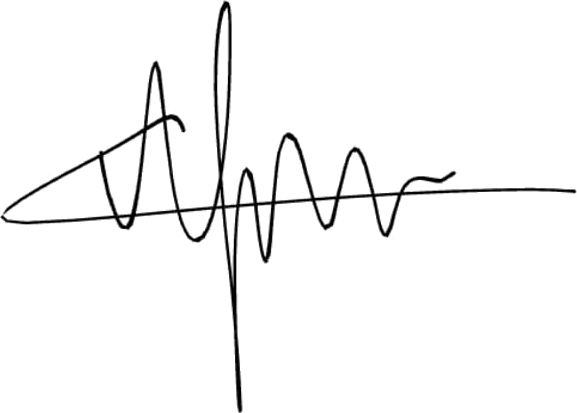
\includegraphics[height=0.8cm]{Figures/signatures/sig_afnan.png}}
\\[6ex]
Name: Saad Riaz Taqi
\\[3ex]
Signature: \raisebox{-0.35\height}{
\includegraphics[height=0.8cm]{Figures/signatures/sig_saad.png}}

\end{flushright}

\vspace{5 cm}

\hrule

\section*{Author's Declaration}
This states Authors' declaration that the work presented in the report is their own, and has not been submitted/presented previously to any other institution or organization.
\pagebreak

\section*{Abstract}
Reconstructing a three-dimensional human face from DNA is an open problem spanning statistical genetics, geometry processing, and machine learning. The recent Difface system mapped single-nucleotide polymorphisms (SNPs) to a 3D facial mesh, but was trained on private data with an unpublished SNP panel, and independent commentary questions whether its accuracy reflects individual genetics or mainly age, gender, and ancestry. FaceCon builds a reproducible genotype-to-3D-face pipeline on documented data, using a documented SNP panel and the shared FLAME representation, and integrates an established forensic DNA phenotyping method, HIrisPlex-S, to provide eye colour, hair colour, and skin colour from the same genotype. It predicts FLAME shape parameters through a baselines-first progression of models measured against demographic baselines, so that any individual-level genetic contribution to facial shape is reported honestly, while eye, hair, and skin colour are obtained by integrating the established HIrisPlex-S method rather than a newly trained appearance model. Controlled access to the real cohort was still pending at the time of writing, so the complete pipeline was implemented and validated on a simulated cohort that follows the public description of the 3D Facial Norms study and carries published facial association signals. On this simulated data the pipeline recovers planted genetic signal, reports none under negative controls, and shows that a simple regularised linear model outperforms the deep models tested. These results establish that the pipeline is correct and ready for real data, and they make no claim about the prediction of real faces.
\pagebreak

\section*{Executive Summary}
FaceCon is a research and development project that explores how much of a person's facial shape can be predicted from their genetic data. Estimating a face from genetic material is relevant to forensic investigation, anthropology, and medical research, and recent progress in artificial intelligence has made the idea newly practical. At the same time, the most visible existing system was built on private data that other researchers cannot check or reuse. Independent experts have also questioned whether its results genuinely reflect individual genetics rather than general characteristics such as age, gender, and ancestry. FaceCon responds to this situation by building an open and carefully evaluated alternative.

The purpose of FaceCon is to provide a transparent and repeatable system that predicts the three dimensional shape of a face from genetic data, using openly documented research datasets rather than private ones. Every step of the process, from preparing the genetic data to measuring the results, is recorded so that others can repeat and verify the work. This openness is the core value of the project, because it gives the research community a trustworthy reference point in a field where strong claims have so far been difficult to confirm.

The proposed solution follows a deliberately cautious strategy. FaceCon begins with very simple prediction methods and moves to more advanced ones only if the simpler methods prove insufficient. Importantly, it always compares its predictions against a basic estimate built only from a person's age, gender, and ancestry. This comparison is what allows the project to separate genuine genetic information from general population patterns and to report honestly how much the genetic data really adds. A fully acceptable and scientifically useful outcome of the project is the finding that genetics adds little beyond this basic estimate under the available data.

Alongside the three dimensional shape of the face, the system also provides a set of visible colour traits, namely eye colour, hair colour, and skin colour, by integrating an established forensic DNA phenotyping method that reads the same genetic data. FaceCon does not train its own method for these colours; it reuses the validated external one and shows its results on the predicted face. The expected outcomes of the project are an open and reusable prediction system, a clear and honest account of facial-shape prediction accuracy and the integrated appearance predictions, and a simple demonstration tool that shows the predicted face next to the real one. The project's limitations are acknowledged from the outset. The genetic and facial data are sensitive and controlled-access, usable records are few, and the data mainly represent certain population groups. For these reasons, FaceCon is positioned as a careful research baseline rather than a finished product, and it does not claim to reconstruct any individual's exact face.

At the time of this deliverable, approval to use the real research data had not yet been granted. The team therefore built the complete system and tested it on a simulated dataset designed to resemble the real study, in which the true answer is known in advance. On this simulated data the system correctly finds genetic information when it is present and correctly reports none when it is absent, which shows that the method can be trusted. The tests were then repeated using real human genetic data from a public reference collection, with the faces still simulated, so that the genetic side of the problem carries the full difficulty of real data. The system behaved in the same way, with the expected reduction in how much it could find. Across all of these tests a simple statistical model predicted better than the more complex neural networks, even when the genetic effects were deliberately made more complicated than a simple model can represent, which suggests that at this data size the way the genetic data is presented matters more than the choice of model. These tests confirm that the system works as designed. They do not yet show how well real faces can be predicted, which is the main work planned for the second phase of the project.

\pagebreak

\pagestyle{fancy}
\tableofcontents

\pagebreak
\listoffigures
\addcontentsline{toc}{chapter}{List of Figures}
\pagebreak
\listoftables
\addcontentsline{toc}{chapter}{List of Tables}

\mainmatter

\chapter{Introduction}
Facial shape is, in part, written in our DNA. Twin studies, heritability analyses, and a growing number of genome-wide association studies (GWAS) have shown that a measurable fraction of the variation in human facial morphology is genetic. Predicting aspects of three-dimensional facial shape from DNA is therefore both a legitimate scientific question and a capability relevant to forensics, anthropology, and medical genetics~\cite{ref:wang,ref:richmond}. Classical work links genotype to face through GWAS and statistical models on facial landmarks or shape scores~\cite{ref:xiong,ref:claes}, while more recent artificial-intelligence systems treat the task as multimodal generation: map genetic variants and facial geometry into a shared representation, then predict a face from genotype~\cite{ref:difface}.

Reconstructing a full 3D face from DNA alone, however, remains an open problem. Difface demonstrated that deep learning can map single-nucleotide polymorphisms (SNPs) to 3D facial meshes~\cite{ref:difface}, but it was trained on private Han Chinese data with an unpublished SNP list, and independent commentary argues that its reported performance may reflect age, gender, and ancestry more than true individual genetic signal, and that evaluation standards in this area are weak~\cite{ref:comment}. Because its data and methods are not fully open, other teams cannot easily verify or reuse the work. FaceCon addresses this gap by building a reproducible SNP to 3D face pipeline on the controlled but documented 3D Facial Norms (3DFN) resource: genotypes from dbGaP and 3D facial scans from FaceBase~\cite{ref:facebase,ref:dbgap}. Rather than copying Difface's fixed 7,842-SNP design and undisclosed mesh template, FaceCon uses its own documented SNP panel and a shared FLAME face representation~\cite{ref:flame}, fitting FaceBase scans to FLAME so that every subject shares one mesh topology, predicting FLAME shape (identity) parameters from genotype, and decoding them to a 3D mesh. Alongside shape, FaceCon integrates an established forensic DNA phenotyping method, HIrisPlex-S~\cite{ref:hirisplex,ref:hirisplexs}, which takes the same dbGaP genotype, extracts its validated marker SNPs, and predicts eye colour, hair colour, and skin colour; these colours are passed to a visualization layer and shown alongside the reconstructed face. FaceCon trains the facial-shape models, whereas the appearance colours come from this external, already-validated predictor rather than a model trained within the project.

\section{Purpose of this Document}
The purpose of this document is to present the problem definition, vision, literature foundation, requirements, methodology, design, prototype implementation, and first experimental results of our Final Year Project (FYP), FaceCon, a research and development system that predicts components of three-dimensional facial shape from genotype, and that integrates an established forensic DNA phenotyping method to provide eye colour, hair colour, and skin colour from the same genotype. The project aims to deliver a reproducible genotype to FLAME pipeline, built on documented, controlled-access data, that measures how much individual facial information DNA carries beyond demographic and population-structure information, and that renders the predicted shape, together with the integrated colour predictions, on a common face model.

Rather than a single question of whether a face can be generated from DNA, the project is organized around a sharper research framing and a set of research questions:

\begin{quote}
Central question: How much individual 3D facial information can be predicted from genotype beyond information already available from demographics and population structure?
\end{quote}

\begin{itemize}
\item (RQ1) Can a reproducible SNP to 3D face pipeline be built on 3DFN/FaceBase with FLAME as the common face representation?
\item (RQ2) How accurately can SNPs predict 3D facial shape versus mean-face and demographic-only baselines?
\item (RQ3) Does adding SNPs to demographics improve 3D facial prediction?
\item (RQ4) Do facial-GWAS-informed SNPs outperform matched random or common SNPs?
\item (RQ5) How do simple statistical and neural models compare with more complex deep models?
\item (RQ6) Which facial regions or FLAME components show the strongest predictable signal?
\item (RQ7) How well does the proposed pipeline generalize across demographic or ancestry subgroups, provided that the final dataset contains sufficient samples for statistically meaningful subgroup evaluation?
\item (RQ8) How can established forensic DNA phenotyping methods be integrated with genotype-based 3D facial shape prediction to provide eye colour, hair colour, and skin colour information alongside the reconstructed face?
\end{itemize}

This document covers the methodology and design through which these questions will be answered, the prototype that implements them, and the first experimental results. Controlled access to the 3DFN data was still pending when this document was written, so every experiment reported here was run on a simulated cohort whose design follows the public description of that study. These experiments establish that the pipeline is correct and ready for the real data. They do not measure how well genotype predicts real faces, which remains the work of the second phase of the project.

\section{Intended Audience}
The intended audience for this report is diverse, and the writing is pitched so that each group can take what it needs. The academic evaluation panel and the project supervisor are the primary audience: they will assess the scientific soundness, novelty, feasibility, and honesty of the work, and will focus on the requirements, methodology, and design chapters as well as the rigor of the evaluation plan. Researchers in facial genetics and 3D computer vision form a second audience who may wish to reproduce or extend the pipeline, and for whom the data choices, SNP-selection procedure, and FLAME representation are described in reproducible detail. Finally, forensic and anthropological practitioners represent an indirect audience who may eventually consume genotype to face methods, and for whom the document is deliberately explicit about what the system can and cannot claim.

\section{Definitions, Acronyms, and Abbreviations}
The following definitions, acronyms, and abbreviations are used throughout this document:

SNP: Single-Nucleotide Polymorphism\\
GWAS: Genome-Wide Association Study\\
3D: Three-Dimensional\\
FLAME: Faces Learned with an Articulated Model and Expressions (a parametric 3D head model)\\
3DFN: 3D Facial Norms (the paired dbGaP genotype and FaceBase scan setting)\\
dbGaP: Database of Genotypes and Phenotypes\\
QC: Quality Control\\
MAF: Minor Allele Frequency\\
HWE: Hardy--Weinberg Equilibrium\\
LD: Linkage Disequilibrium\\
PC: Principal Component\\
MLP: Multi-Layer Perceptron\\
CLIP: Contrastive Language--Image Pre-training (a contrastive alignment method)\\
MSE/RMSE/MAE: Mean Squared Error / Root Mean Squared Error / Mean Absolute Error\\
OBJ: a 3D geometry file format\\
SDG: Sustainable Development Goal\\
FYP: Final Year Project\\
MVP: Minimum Viable Product

\section{Conclusion}
This chapter introduced FaceCon as a reproducible, honestly-evaluated genotype to 3D face and appearance system, stated the purpose of the document and the research questions, identified the intended audiences, and defined the key terminology. The remainder of the report is organized as follows. Chapter~2 sets out the project vision: the problem domain, the problem statement and its sub-problems, the goals, scope, targeted Sustainable Development Goals, constraints, opportunity, and stakeholders. Chapter~3 reviews the literature on facial genetics and the methods the system depends on. Chapter~4 specifies the software requirements, use cases, interface, and risks. Chapter~5 presents the proposed methodology as a documented, reproducible pipeline. Chapter~6 presents the high-level and low-level design that realizes that methodology. Chapter~7 describes the implemented prototype and its test cases. Chapter~\ref{ch:results} reports and discusses the experimental results obtained on simulated data. Chapter~\ref{ch:conclusion} concludes the report and sets out the plan of work for FYP-II.

\chapter{Project Vision}
\label{ch:vision}
This chapter describes what FaceCon does, the problem it solves, and the goals, scope, and stakeholders that bound it. FaceCon is a research and development project that predicts components of three-dimensional facial shape from genotype, and that integrates an established forensic DNA phenotyping method (HIrisPlex-S) to provide eye colour, hair colour, and skin colour from the same genotype, on documented and controlled-access data, with a shape evaluation designed to separate genuine genetic signal from demographic and ancestry-related signal.

\section{Problem Domain Overview}
The problem domain of FaceCon lies at the intersection of statistical genetics, three-dimensional geometry processing, and machine learning. Human facial morphology is a highly polygenic and moderately heritable trait: many genetic loci each contribute a small effect, and their combined influence is entangled with age, gender, and population ancestry. Predicting a face from a genome is therefore a layered inference problem. One must first decide which genetic variants to use, then decide how to represent a face so that it can be learned and generated, and finally build a model that connects the two while accounting for confounders. FaceCon takes genotype data (an SNP dosage matrix), optional demographic covariates, and 3D facial scans standardized through the FLAME model, and it learns to predict FLAME shape parameters that decode into a 3D facial mesh. The system then evaluates those predictions quantitatively against carefully chosen baselines.

\section{Problem Statement}
Existing state-of-the-art genotype to 3D face systems, most notably Difface, achieve their results on private data using undisclosed SNP panels, undocumented mesh formats, and unreleased weights, and their reported individual-level accuracy has been challenged as potentially attributable to demographic confounders rather than genuine genetic signal. There is, at present, no open, reproducible, and demographically controlled baseline that predicts 3D facial shape from genotype on publicly documented data.

\section{Problem Elaboration}
The problem decomposes into four coupled sub-problems that FaceCon must address. They are coupled because a solution to any one of them is of little use without the others: a reproducible pipeline with an inflated evaluation would mislead, and an honest evaluation is meaningless without a shared face representation on which predictions can be compared. Each is described in turn below.

First, the reproducibility gap. Existing state-of-the-art systems such as Difface cannot be fully reproduced from the publicly available artifacts, because important elements of the data, preprocessing pipeline, SNP configuration, and model resources are not openly available. FaceCon therefore requires a pipeline constructed from clearly documented components and reproducible processing steps.

Second, the representation mismatch. Difface uses a fixed SNP configuration and a dense 3D facial representation that do not directly correspond to the genotype and facial data available in 3DFN/FaceBase. FaceCon must therefore define its own genetic input representation and standardized geometric output. This project uses a documented SNP-selection procedure and FLAME shape parameters as a common representation of 3D facial structure.

Third, demographic and population confounding must be addressed. Variables such as age, gender, and ancestry are associated with systematic variation in facial morphology and may account for part of the apparent predictive performance of genotype models. FaceCon therefore evaluates demographic-only, genotype-only, and combined models in order to estimate the incremental predictive contribution of genetic information beyond demographic and population-level structure.

Fourth, data access and sample size impose practical constraints. Paired genotype and 3D facial data are sensitive, relatively scarce, and typically available through controlled-access resources. The modelling strategy must therefore account for the number and distribution of usable paired subjects in the final dataset. Model complexity will be matched to the available data and evaluated against simpler statistical and neural baselines, while the statistical limitations of the resulting experiments will be explicitly reported.

\section{Goals and Objectives}
\label{sec:goals}
The goal of FaceCon is to deliver an open, documented, and demographically controlled pipeline for genotype to 3D face prediction. The specific objectives are to:

\begin{itemize}
\item Build a reproducible genotype to FLAME pipeline on paired 3DFN subjects.
\item Document genotype QC and construct a transparent, GWAS-informed SNP panel.
\item Document scan to FLAME fitting so that training targets are comparable across subjects.
\item Implement and compare progressively more complex models, including mean-face and demographic baselines, statistical SNP models, MLPs, and transformer models.
\item Evaluate predictions rigorously with parameter, mesh, landmark, region, and retrieval metrics, plus ablations.
\item Separate genetic contribution from demographic and ancestry-related signal, and report it honestly.
\item Provide eye colour, hair colour, and skin colour alongside the reconstructed face by integrating an established forensic DNA phenotyping method (HIrisPlex-S) that uses the same genotype, rather than training a new appearance model.
\item Provide clear limitations and an ethical discussion, and a working visualization or system demonstration.
\end{itemize}

Success does not require photorealistic skin texture or a fully photorealistic rendering, operational forensic identification, beating Difface on its private dataset, or a diffusion model or large Transformer by default. A scientifically valid outcome may be that simple models match or beat complex ones, or that SNPs add little predictive value beyond demographics under the evaluated conditions.

\section{Project Scope}
The scope of this project is to design, build, and evaluate a reproducible system that predicts 3D facial shape parameters from genotype on the 3DFN resource. The project will:

\begin{itemize}
\item Use 3DFN subjects who have both dbGaP genotypes and FaceBase 3D scans.
\item Clean genotypes through documented QC and reduce them to a documented SNP panel.
\item Register FaceBase scans to FLAME so each subject is one common mesh, with FLAME shape parameters as the training target.
\item Train a progression of models from mean-face and demographic baselines through statistical and neural SNP models.
\item Decode predicted FLAME parameters to 3D meshes and evaluate them quantitatively against baselines, with ablations and region analysis.
\item Deliver preprocessing and prediction software with reproducible configurations, evaluation figures, and a working demonstration.
\end{itemize}

The project scope includes eye colour, hair colour, and skin colour, obtained by integrating the established HIrisPlex-S forensic DNA phenotyping method, which uses the same genotype as the shape pipeline; these colours are rendered or reported alongside the predicted face. FaceCon does not train its own appearance model and does not predict other appearance traits such as freckling, hair type, or male-pattern baldness. The project scope does not include photorealistic skin texture or a fully photorealistic rendering, DNA-methylation-based age estimation, operational forensic identification, claims that DNA uniquely reconstructs a person's exact face, the use of any data outside approved controlled-access agreements, or a requirement to employ large generative models. The preferred wording for all claims is that the system predicts components of 3D facial morphology from genotype, and integrates established forensic phenotyping to report eye, hair, and skin colour, under the evaluated dataset and conditions.

\section{Sustainable Development Goal (SDG)}
FaceCon aligns most directly with SDG 9: Industry, Innovation and Infrastructure, because it contributes open, reproducible research infrastructure and methodology to an emerging area of applied artificial intelligence. By releasing documented code and models rather than closed artifacts, the project strengthens the shared scientific infrastructure on which future genotype to face research can build. The project also relates to SDG 3: Good Health and Well-being, through the relevance of genotype to craniofacial shape modeling to the study of developmental and craniofacial conditions. The two relevant goals are shown in Figure~\ref{fig:1}.

\begin{figure} [!h]
    \centering

\includegraphics[width=0.5\textwidth]{Figures/sdg_relevant}
    \caption[Sustainable Development Goals targeted by FaceCon]{SDG 3, Good Health and Well-being (green tile, left), and SDG 9, Industry, Innovation and Infrastructure (orange tile, right), targeted by FaceCon.}
    \label{fig:1}
\end{figure}

\section{Constraints}
The project operates under several constraints. Data constraints: the primary data are controlled-access (FaceBase and dbGaP), limited in sample size, and drawn largely from specific ancestry groups, which bounds statistical power and generalization. The exact usable paired sample count is unknown until access and QC are complete. Ethical and legal constraints: genotype and facial data are sensitive, so all use must remain within approved data-use agreements, with no attempt at re-identification. Computational constraints: routine development, preprocessing, baseline models, and smaller neural experiments should remain feasible on available student hardware, while more demanding training can use university GPU resources. Time constraints: the project must remain achievable within the final-year project timeline. Scientific constraints: model complexity and evaluation must remain appropriate to the size and quality of the available dataset, and conclusions must reflect the level of predictive accuracy supported by the results.

\section{Business Opportunity}
Although FaceCon is a research and development project rather than a commercial product, it addresses a genuine opportunity. Forensic laboratories, anthropological research groups, and medical-genetics teams increasingly seek tools that relate genetic samples to physical appearance, and there is clear demand for methods that are transparent and auditable rather than opaque. An open, reproducible baseline lowers the barrier to entry for these organizations, provides a reference implementation against which future or commercial tools can be validated, and creates a foundation for further, better-resourced work. The opportunity is therefore one of enabling infrastructure and trust rather than of a directly monetized service.

\section{Stakeholders Description / User Characteristics}
This section identifies the users and stakeholders of the system and their roles. Because FaceCon is a research system and not a product, its direct users are few and technical, but its results concern a wider group, including the participants whose data it would use and the forensic and clinical communities who might later rely on work of this kind. The summary below lists each group, and the following subsection sets out what each needs from the project.

\subsection{Stakeholders Summary}
The stakeholders of FaceCon are the project team and supervisor, who develop and supervise the system, and the academic evaluators, who assess it. Beyond the university, they include the broader research community in facial genetics and 3D vision, who may reuse and extend the open pipeline, and, more distantly, the forensic, anthropological, and medical-genetics practitioners who represent the eventual application domains. The direct users of the system are the researcher-developer, who runs the pipeline, and the evaluator, who inspects results. A demonstration user may additionally submit a test-subject genotype and view the predicted face.

\subsection{Key High-Level Goals and Problems of Stakeholders}
The project team and supervisor aim to deliver a technically sound, reproducible system within the available time and data, and their central problem is balancing ambitious modeling against honest, confounder aware evaluation on limited data. The academic evaluators aim to assess novelty, rigor, and completeness, and are concerned that claims are supported by the evaluation. The research community wants an open baseline it can verify and extend, a need unmet by current closed systems. Practitioners want transparent tools and, above all, an honest statement of the demographically controlled reliability of any prediction.

\section{Conclusion}
This chapter has set out the vision for FaceCon. Its central commitment is that the project measures how much genotype adds to facial prediction beyond age, sex, and ancestry, rather than how well a face can be produced from DNA, because a system can appear accurate while reproducing only what demographics already reveal. That commitment shapes everything that follows. It narrows the scope to predicting components of facial shape and to integrating an established forensic method for eye, hair, and skin colour, and it rules out any claim to identify individuals. The goals and objectives were stated so that each could later be checked against what was achieved, and the constraints were recorded honestly: the data are sensitive, controlled, limited in size, and drawn largely from one ancestry, and these limits bound what any result can show. The project serves SDG~9 through open, reproducible research infrastructure and SDG~3 through its relevance to craniofacial research. The next chapter reviews the literature that motivates this vision and the methods on which it depends.

\chapter{Literature Review / Related Work}
This chapter reviews the research that motivates and enables FaceCon. Because FaceCon is a research and development project, a detailed and critical literature survey is provided rather than a catalogue of competing products. The review is organized topic by topic, moving from the biology of facial genetics through to the methods the system depends on. Within each topic, every research item is reviewed separately under three headings: a Summary of what the work proposes and finds, a Critical Analysis of its strengths and limitations, and a statement of its Relationship to the Proposed Work. Each topic then closes with a short synthesis that draws its papers together and connects them to FaceCon.

\section{Definitions, Acronyms, and Abbreviations}
This chapter uses the terms defined in Chapter~1, together with the following. Genotype is the set of genetic variants carried by an individual. Phenotype is an observable trait such as facial shape. Locus is a position in the genome. Heritability is the proportion of trait variation attributable to genetic variation. Mesh is a set of vertices and faces describing a 3D surface. Morphable model is a parametric model that represents a family of shapes as a low-dimensional vector. Contrastive learning is training that pulls matched pairs together and pushes unmatched pairs apart in a shared embedding space.

\section{Detailed Literature Review}
The review is grouped into topics that trace the path from the biology of facial genetics to the methods FaceCon depends on. Each topic opens with its most relevant works, reviews every item under the same three headings, and closes with a short synthesis that draws out the implications for FaceCon.

\subsection{Genetic Prediction of Facial Morphology}
This topic covers the genome-wide association studies that establish, biologically, that facial shape is partly heritable, and that identify the variants a predictive model can draw on.

\subsubsection{Claes et al. --- Global to Local Genetic Effects on Facial Shape}
Summary. Claes et al.~\cite{ref:claes} propose a data-driven, global to local approach for discovering how genetic variants influence facial shape. The objective is to move beyond simple landmark distances and to localize genetic effects to specific facial regions. Methodologically, the work hierarchically segments three-dimensional facial shape into progressively finer regions and performs a multivariate genome-wide association study on each segment, relating genome-wide SNPs to the shape of each region. The data combine three-dimensional facial images with genome-wide genotyping for cohorts of predominantly European ancestry. The study identifies multiple genomic loci associated with facial shape, several of them novel, and shows that distinct loci act on distinct parts of the face.

Critical Analysis. The principal strength of the work is methodological: the multivariate, region design captures effects that univariate landmark studies miss, and the resulting loci are published and reproducible. Its main limitation for a prediction project is that it is oriented toward discovery rather than generation, so it identifies associations without delivering an end-to-end face predictor. The cohort is ancestry-concentrated, which limits the transfer of specific effect sizes to other populations, and, as with all facial genetics, the effects are individually small and highly polygenic.

Relationship to the Proposed Work. FaceCon adopts the face-associated loci reported in this line of work as part of the evidence base for its documented SNP panel, rather than copying an undisclosed panel. It differs by building a generative genotype to FLAME predictor instead of an association map, and it directly inherits the study's caution about ancestry generalization, which it addresses through stratified evaluation. The work therefore influences FaceCon's SNP-selection stage rather than its modelling architecture.

\subsubsection{White et al. --- Genetic Architecture of the Human Face}
Summary. White et al.~\cite{ref:white} extend segment facial genetics with a multivariate genome-wide association study that expands the catalogue of face-associated variants and clarifies how genetic effects are distributed across the face. The approach again pairs three-dimensional facial phenotyping with genome-wide genotypes in predominantly European cohorts, and it contributes a richer map of which genomic regions influence which aspects of facial morphology.

Critical Analysis. The study's strength is the breadth of its catalogue and the rigor of its multivariate analysis, which strengthen the evidence that facial shape is genetically structured. Its limitations mirror those of the topic as a whole: it remains discovery-oriented rather than predictive, its cohorts are ancestry-concentrated, and the polygenic, small-effect nature of the signal means that individual-level prediction is not demonstrated.

Relationship to the Proposed Work. FaceCon uses this expanded catalogue as a second pillar of its SNP-panel evidence base, alongside Claes et al. It modifies the role of these associations by treating them as candidate predictive features rather than endpoints, and it differs by predicting full FLAME shape. The work helps FaceCon justify a GWAS-informed panel and provides the comparison point for the ablation against matched-random SNPs.

\subsubsection{Naqvi et al. --- Shared Heritability of Face and Brain Shape}
Summary. Naqvi et al.~\cite{ref:naqvi} investigate the genetic overlap between facial and brain shape. Using genome-wide analysis and genetic-correlation methods on European cohorts, the study shows that many loci influencing the face also relate to cranial and neuroanatomical variation, deepening the understanding of the developmental genetics that couples facial form to underlying structure.

Critical Analysis. The work's strength is that it establishes the biological embedding of facial genetics within broader craniofacial development, which supports the plausibility of predicting shape from genotype. Its relevance to prediction is indirect, however, because it characterizes genetic overlap rather than reconstructing faces, and like the other studies it is concentrated in a single ancestry group.

Relationship to the Proposed Work. This study provides part of the biological rationale that FaceCon cites for attempting genotype to shape prediction, and it informs which loci are most likely to carry shape-relevant signal. FaceCon does not adopt a method from it, but uses it to motivate the scientific premise and to reinforce the expectation that the predictable signal is diffuse.

\subsubsection{Xiong et al. --- Combined GWAS and Facial Prediction}
Summary. Xiong et al.~\cite{ref:xiong} present a combined genome-wide association study of facial traits in Europeans whose explicit objective is to increase explained variance and to improve facial prediction. The methodology analyses close to one thousand facial measurements in over eleven thousand individuals, combining cohorts to boost power, and couples association discovery with prediction modelling. The study reports a large number of associated genomic regions, including many previously unknown, explains substantially more genetic variance than earlier work, and demonstrates improved facial prediction, extending even to the reconstruction of archaic human facial profiles.

Critical Analysis. This is among the most prediction-oriented facial-genetics studies, and its explicit treatment of prediction and cross-population validation is a model for careful reporting. Its limitations are that it operates on facial measurements and landmarks rather than full generative 3D meshes, and that it remains concentrated in European ancestry, so its prediction performance may not transfer directly to other populations.

Relationship to the Proposed Work. Xiong et al. serve FaceCon both as an SNP-selection resource and as a methodological benchmark for honest, prediction-focused reporting. FaceCon extends this line of work from measurement-level prediction into generative 3D FLAME prediction, and it adopts the study's discipline of reporting prediction against clear reference points, which FaceCon implements as its demographic baselines.

\subsubsection{Richmond et al. --- Overview of Facial Genetics}
Summary. Richmond et al.~\cite{ref:richmond} provide an accessible review of facial genetics. The work summarizes heritability evidence, the growth of facial genome-wide association studies, and the clinical and forensic relevance of predicting appearance from DNA, consolidating the field for a broad audience.

Critical Analysis. As a review, its strength is a balanced, consolidated overview that situates the individual studies within a coherent picture. Its limitation is that it contributes no new model or dataset, so it informs context rather than method.

Relationship to the Proposed Work. FaceCon uses this review to frame the problem domain and to justify the relevance of genotype to face research. It adopts no technique from it, but draws on it to motivate the project and to set realistic expectations about what facial genetics can and cannot currently achieve.

Synthesis. Collectively, these studies establish that facial morphology is genetically influenced and polygenic, and they provide reproducible, published associations between variants and facial traits. They share two limitations that shape FaceCon directly: they are largely discovery- or measurement-oriented rather than generative, and they are ancestry-concentrated. None provides an open, generative 3D predictor. This is the research gap that FaceCon targets, and it is why FaceCon builds a transparent, GWAS-informed SNP panel and commits in advance to ancestry-stratified evaluation.

\subsection{Forensic DNA Phenotyping}
This topic covers the applied setting in which appearance is predicted from DNA, which is where genotype to face research is ultimately motivated.

\subsubsection{Wang et al. --- A 19-SNP Forensic Prediction System}
Summary. Wang et al.~\cite{ref:wang} describe a forensic DNA-phenotyping system based on a compact nineteen-SNP panel for predicting externally visible characteristics. The work follows the established forensic pattern of selecting and validating a small, interpretable panel for categorical appearance traits so that predictions can support investigations from unidentified genetic material.

Critical Analysis. The strength of this approach is its rigor and deployability: a small validated panel is interpretable, inexpensive to genotype, and suited to casework. Its limitation, from FaceCon's perspective, is that it predicts discrete traits such as pigmentation rather than continuous three-dimensional facial geometry, so it addresses a much narrower output than full facial shape.

Relationship to the Proposed Work. FaceCon shares the forensic and anthropological motivation of this work and targets the harder output of continuous 3D facial shape, while integrating, rather than retraining, established forensic phenotyping to provide the categorical colour traits (eye, hair, and skin colour) alongside the reconstructed face. It adopts the forensic discipline of small, documented, validated panels for appearance while remaining explicitly scoped as research with firm limits on individual-level claims. The work helps define both the appearance method FaceCon integrates and the shape gap it explores.

\subsubsection{HIrisPlex-S --- Eye, Hair, and Skin Colour Prediction}
Summary. The HIrisPlex and HIrisPlex-S systems~\cite{ref:hirisplex,ref:hirisplexs} predict eye and hair colour, and subsequently skin colour, from compact validated SNP panels, and are the de facto standard for appearance prediction in forensic genetics. Complementary genome-wide association work in admixed cohorts~\cite{ref:adhikari} further characterises the genetic basis of human pigmentation across diverse populations.

Critical Analysis. These systems are rigorously validated and report calibrated, honest performance, which is strong at the pigmentation extremes (for example blue and brown eyes, pale and dark skin, red and black hair) and genuinely weaker for intermediate categories. Their scope is categorical appearance rather than 3D geometry, and performance is partly entangled with ancestry.

Relationship to the Proposed Work. FaceCon's appearance component follows this literature by integrating the established HIrisPlex-S predictor directly: the same genotype supplies HIrisPlex-S's validated marker SNPs, and the external predictor returns eye colour, hair colour, and skin colour, which are shown alongside the reconstructed face. FaceCon does not retrain these forensic models or extend them to other traits, and it reports their colours using the published method rather than re-deriving accuracy on its own data.

Synthesis. The forensic literature demonstrates both the demand for genotype to appearance prediction and the discipline with which it is usually approached, through small validated panels, categorical traits, and honest calibration. FaceCon incorporates this appearance line of work as a dedicated module and combines it with continuous 3D shape prediction, positioning itself across both while refusing to present itself as an operational identification tool.

\subsection{Statistical and Learning Methods for Genotype to Face Prediction}
This topic covers approaches that connect genotype and face using statistical and learning models, which form FaceCon's essential baselines and its closest methodological neighbours.

\subsubsection{Sero et al. --- Face to DNA Classifiers}
Summary. Sero et al.~\cite{ref:sero} take a complementary, face to DNA direction. The objective is to quantify how much genomic information is recoverable from a face by building classifiers that predict DNA-encoded attributes (such as genomic background and individual loci) and DNA-inferred attributes (such as age) from three-dimensional faces, and then matching individuals between the two modalities. The data pair 3D facial images with genomic data across both diverse and more homogeneous cohorts, and the study reports verification-mode matching rates well above chance, on the order of eighty percent.

Critical Analysis. The study is rigorous and quantitative, and its most valuable feature is its honesty: the authors show that much of the matching signal is carried by broad attributes such as gender and ancestry rather than by fine individual genetics. Its limitations are that it works in the reverse (face to DNA) direction rather than generating a face, that verification is weaker than individual identification, and that the demographic contribution it exposes is a warning about how easily apparent performance can be overstated.

Relationship to the Proposed Work. This work is, in effect, a specification for part of FaceCon's evaluation. FaceCon adopts its central lesson by making demographic baselines mandatory and by decomposing performance into demographic and individual-genetic components. FaceCon differs by predicting in the forward direction, from genotype to 3D shape, and by using the demographic decomposition not as an afterthought but as the headline measure of success.

Synthesis. Statistical and learning methods are interpretable, sample-efficient, and often competitive when paired sample sizes are modest, which is exactly the regime FaceCon expects. The decisive lesson of this topic is that demographic attributes can dominate apparent performance unless they are explicitly controlled, which is why FaceCon adopts ridge regression and demographic regressors as mandatory baselines and builds the demographic-versus-genetic decomposition directly into its evaluation.

\subsection{Deep Learning for Genotype to Face Generation}
This topic covers the neural systems that treat genotype to face as multimodal generation, together with the critique and the broader guidance that shape how such systems should be built and judged.

\subsubsection{Jiao et al. --- Difface}
Summary. Jiao et al.~\cite{ref:difface} propose Difface, the most visible recent system for DNA to 3D face generation. The objective is to reconstruct a dense three-dimensional facial mesh from DNA alone. Methodologically, Difface is a two-stage, multi-modality model: it first contrastively aligns a transformer SNP encoder with a mesh face encoder, and it then uses a diffusion prior in the shared embedding space to reconstruct the mesh. It was trained on roughly 9,674 Han Chinese subjects using about 7,842 GWAS-selected SNPs, and it demonstrates that modern generative models can map genotype to a recognizable 3D face.

Critical Analysis. Difface is a compelling proof of concept and combines several strong ideas, but its limitations are decisive for reproducibility and for scientific interpretation. Its public release does not provide the SNP list, the full preprocessing, the face template, or reusable pretrained weights, so it cannot be independently reproduced. Its evaluation does not cleanly separate individual-level prediction from demographic averages, its cohort is drawn from a single ancestry group, and its dense-mesh target is high-dimensional and tied to an undocumented topology.

Relationship to the Proposed Work. FaceCon treats Difface as an architectural reference rather than a system to reproduce. It adopts the high-level two-stage alignment and generation idea, but it re-implements the pipeline on documented 3DFN and FaceBase data, replaces the undisclosed panel with a documented SNP-selection procedure, substitutes the shared FLAME representation for the unknown dense mesh, and, most importantly, adds the demographic baselines whose absence is Difface's central evaluation weakness. FaceCon therefore directly targets the reproducibility and confounding gaps that Difface leaves open.

\subsubsection{Wagner et al. --- Critique of Difface}
Summary. Wagner et al.~\cite{ref:comment} respond to Difface with a critical commentary. The work argues that facial-genetics AI systems require transparent metrics, clear disclosure of data flow, and evaluation that explicitly separates demographic signal from individual genetic prediction, and it uses Difface as a case study for these requirements.

Critical Analysis. The commentary's strength is that it names, precisely, the methodological trap that the whole subfield must avoid, turning a general concern into a concrete evaluation requirement. Its limitation is that, as a commentary, it diagnoses the problem rather than providing an open system that demonstrates the solution.

Relationship to the Proposed Work. FaceCon operationalizes this critique. The requirements it raises, transparency, disclosed data flow, and confounder separated evaluation, become concrete design commitments in FaceCon's methodology, and in particular its demographic-baseline-centered evaluation is a direct response to the concerns raised here.

\subsubsection{Alharbi and Rashid --- Deep Learning in Human Genomics}
Summary. Alharbi and Rashid~\cite{ref:alharbi} survey deep learning in human genomics using next-generation sequencing data. The review maps the architectures, tasks, and recurring challenges of the field, with particular attention to convolutional, recurrent, and attention models and to the practical problems of data scarcity, confounding, and interpretability.

Critical Analysis. The survey's strength is an up-to-date and balanced account of methods and pitfalls, which is directly relevant to a small-sample genotype to face project. Its limitation is that it is broad and does not address the specific genotype to 3D shape task, so its lessons must be adapted rather than applied directly.

Relationship to the Proposed Work. This review justifies FaceCon's methodological caution. Its warnings about data scarcity and confounding support FaceCon's decision to prefer compact models, to evaluate complex architectures only against simpler baselines, and to treat interpretability and honest reporting as first-class concerns.

Synthesis. FaceCon treats Difface as an architectural reference, particularly its two-stage alignment and generation framework, while adapting the modelling approach to the 3DFN dataset and FLAME representation. It incorporates the evaluation considerations raised by Wagner et al. and the cautions of Alharbi and Rashid regarding model complexity and limited sample sizes.

\subsection{3D Facial Representations and FLAME}
This topic covers how a 3D face can be represented so that it is comparable across subjects and usable as a learning target.

\subsubsection{Egger et al. --- Survey of 3D Morphable Models}
Summary. Egger et al.~\cite{ref:egger} survey two decades of 3D morphable face models, covering how they are constructed, fitted, and applied, and situating modern parametric models within that history. The survey provides a comprehensive and authoritative map of the representational landscape in which FLAME sits.

Critical Analysis. Its strength is breadth and authority, giving a balanced account of what morphable models can and cannot do. Its limitation is that, being published before the most recent neural generative advances, it only anticipates some of the directions that are now central.

Relationship to the Proposed Work. This survey frames FaceCon's representational choice and clarifies the trade-offs, particularly the loss of fine detail, that come with a compact parametric target. It justifies, at a conceptual level, FaceCon's decision to predict a morphable-model parameterization rather than raw geometry.

\subsubsection{Li et al. --- The FLAME Head Model}
Summary. Li et al.~\cite{ref:flame} propose FLAME, a parametric head model with a linear identity shape space, expression blendshapes, and pose, learned from thousands of 3D head scans. FLAME represents any face as a short parameter vector and decodes that vector back into a full mesh with a fixed, shared topology.

Critical Analysis. FLAME's strengths are topological consistency and a compact, interpretable parameterization that is well suited to learning. Its limitations are a ceiling on fine detail inherent to a linear shape space and a dependence on the demographic composition of its training scans, which can bias the representable range of faces.

Relationship to the Proposed Work. FLAME is the backbone of FaceCon's face representation. FaceCon adopts FLAME directly: it registers every FaceBase scan to FLAME so that all subjects share a topology, and it predicts FLAME identity parameters as its learning target. This choice is what makes the generative problem compact and comparable across models.

\subsubsection{Feng et al. --- DECA}
Summary. Feng et al.~\cite{ref:deca} present DECA, which learns to regress a detailed, animatable 3D face model from unconstrained single images. Building on a FLAME-style parameterization, DECA uses a detail-consistency loss to separate person-specific shape detail from expression-dependent variation, and it recovers convincing geometry even from weak, in-the-wild inputs.

Critical Analysis. DECA's strength is its demonstration that a FLAME target pairs effectively with a learned encoder under difficult input conditions. Its limitation, for FaceCon, is that its input modality is images rather than genotype, and its fine detail relies on image-texture cues that have no analogue in DNA, so only its representational strategy transfers.

Relationship to the Proposed Work. DECA validates the design choice at the heart of FaceCon's output, namely pairing a FLAME parameterization with a learned encoder-decoder. Where DECA regresses FLAME from pixels, FaceCon generates FLAME from genotype, but both rely on the same compact, topology consistent target, and DECA's success on weak inputs is encouraging for an even weaker conditioning signal.

\subsubsection{Gong et al. --- SpiralNet++}
Summary. Gong et al.~\cite{ref:spiralnet} propose SpiralNet++, an efficient spiral mesh-convolution operator for neural networks that consume meshes of fixed topology. It defines local neighbourhoods along spirals on a mesh and aggregates them efficiently, providing a simple and fast operator for mesh learning.

Critical Analysis. Its strength is efficiency and simplicity for fixed-topology meshes. Its limitation is precisely that it assumes a fixed vertex ordering, which is only available after registration to a common template, so it cannot be applied to raw, uncorresponded scans.

Relationship to the Proposed Work. SpiralNet++ becomes applicable to FaceCon only because every scan is registered to the shared FLAME topology. It is a candidate operator for an advanced mesh encoder, and it illustrates why the FLAME registration step is a prerequisite for mesh-convolutional models within FaceCon.

Synthesis. This topic supplies FaceCon's output representation. Morphable models, and FLAME in particular, give the topological consistency and compactness that make 3D faces learnable; DECA shows the target pairs well with learned encoders; and SpiralNet++ becomes usable once scans are registered to a common FLAME topology. FaceCon therefore fits every FaceBase scan to FLAME and predicts FLAME shape parameters, accepting reduced fine detail in exchange for a tractable, comparable learning target.

\subsection{Advanced Representation and Generative Modeling Methods}
For the advanced modelling stage, FaceCon considers modern representation-learning and generative approaches. Denoising diffusion probabilistic models~\cite{ref:ddpm} learn to reverse a gradual noising process to generate samples, while latent diffusion~\cite{ref:ldm} performs this process in a learned lower-dimensional representation to reduce computational cost and support conditional generation. Contrastive learning, as popularized by CLIP~\cite{ref:clip}, can align two different modalities within a shared feature space. Transformer architectures~\cite{ref:transformer} use self-attention to model interactions across input features and can be adapted to SNP data using suitable embeddings and genomic positional information.

Critical Analysis. These methods provide greater modelling capacity but also introduce higher data and computational requirements. This is particularly relevant for genotype to face prediction, where the number of paired subjects is small relative to the dimensionality of the genetic input. More complex architectures must therefore be evaluated against simpler statistical and neural baselines to determine whether their additional capacity produces meaningful improvements.

Relationship to the Proposed Work. FaceCon follows a progressive modelling strategy from statistical SNP models to MLPs and transformer models. Contrastive alignment will be investigated for learning shared SNP-face representations, while generative approaches such as diffusion will be evaluated where the size of the final paired dataset and preceding experimental results support their use.

\subsection{Datasets and Tooling}
This topic covers the data resources and tools that make a reproducible pipeline possible. The 3D Facial Norms Database provides high-quality craniofacial anthropometry and 3D facial surface models through the FaceBase consortium~\cite{ref:facebase}, and genotypes for related normal facial variation are available through dbGaP accession phs000949~\cite{ref:dbgap}. Genotype quality control and SNP handling are supported by standard, community-maintained tooling~\cite{ref:plink}. The strength of this setting is that it is documented and reusable, unlike the private cohorts of closed systems, while its limitations are modest sample size and ancestry concentration. These resources are FaceCon's data foundation, and using them is precisely what allows the whole pipeline to be reproduced by others.

\section{Literature Review Summary Table}
Table~\ref{tab:litsummary} summarizes the reviewed research in the research-project format of author, method, results or contribution, and limitations.

{\small\setlength{\LTpre}{6pt}\setlength{\LTpost}{0pt}
\begin{longtable}{|p{2.6cm}|p{3.5cm}|p{4.0cm}|p{3.2cm}|}
\caption{Summary of the literature reviewed for FaceCon (research-project format).}\label{tab:litsummary}\\
\hline
\textbf{Author} & \textbf{Method} & \textbf{Results / Contribution} & \textbf{Limitations} \\ \hline
\endfirsthead
\hline
\textbf{Author} & \textbf{Method} & \textbf{Results / Contribution} & \textbf{Limitations} \\ \hline
\endhead
\hline
\endfoot
Claes et al.~\cite{ref:claes} & Global to local segmented GWAS & Many novel facial-shape loci; localized effects & Discovery-oriented; ancestry-concentrated \\ \hline
White et al.~\cite{ref:white} & Multivariate facial GWAS & Expanded catalogue of face-associated variants & Mostly European cohorts \\ \hline
Naqvi et al.~\cite{ref:naqvi} & GWAS / shared-heritability analysis & Links face and brain shape genetics & Indirect for prediction \\ \hline
Xiong et al.~\cite{ref:xiong} & Combined GWAS + prediction & More explained variance; improved prediction & Landmark/measurement; European \\ \hline
Richmond et al.~\cite{ref:richmond} & Review of facial genetics & Accessible overview of loci and relevance & Not a predictive model \\ \hline
Wang et al.~\cite{ref:wang} & 19-SNP forensic prediction system & Validated categorical-trait prediction & Categorical traits only; not 3D shape \\ \hline
Sero et al.~\cite{ref:sero} & Face to DNA classifiers & Above-chance verification matching & Signal partly demographic; not full 3D generation \\ \hline
Jiao et al.~\cite{ref:difface} & Transformer + mesh encoder; diffusion prior & First de novo 3D-face reconstruction from DNA & Private data; undisclosed panel/weights; weak demographic control \\ \hline
Wagner et al.~\cite{ref:comment} & Critical commentary & Specifies transparent, confounder aware evaluation & Diagnoses rather than provides a system \\ \hline
Alharbi \& Rashid~\cite{ref:alharbi} & Survey of deep learning in genomics & Maps methods, pitfalls, confounding & Not specific to 3D-shape prediction \\ \hline
Egger et al.~\cite{ref:egger} & Survey of 3D morphable models & Comprehensive map of the field & Pre-dates recent neural methods \\ \hline
Li et al.~\cite{ref:flame} & FLAME parametric head model & Compact, topology consistent shape space & Linear; limited fine detail; population bias \\ \hline
Feng et al.~\cite{ref:deca} & FLAME + learned encoder (DECA) & Detailed 3D face from in-the-wild images & Image inputs, not genotype \\ \hline
Gong et al.~\cite{ref:spiralnet} & SpiralNet++ mesh convolution & Fast, efficient mesh operator & Requires fixed topology \\ \hline
Rombach et al.~\cite{ref:ldm} & Latent diffusion & Efficient, controllable generation & Needs large data; conditioning quality matters \\ \hline
Radford et al.~\cite{ref:clip} & Contrastive multimodal alignment & Shared cross-modal embedding space & Scales with paired-data volume \\ \hline
Ho et al.~\cite{ref:ddpm} & Denoising diffusion (DDPM) & High-quality generative modeling & Data- and compute-intensive \\ \hline
Vaswani et al.~\cite{ref:transformer} & Transformer self-attention & Strong sequence/feature encoder & Data-hungry on small panels \\ \hline
Chang et al.~\cite{ref:plink} & Second-generation PLINK & Standard genotype QC toolkit & Scientific thresholds left to user \\ \hline
\end{longtable}
}

\section{Conclusion}
Taken together, the literature both justifies FaceCon and constrains its design. The facial-GWAS studies establish that facial shape is genetically influenced and supply a transparent evidence base for SNP selection, yet they are discovery- or measurement-oriented and ancestry-concentrated rather than generative. Forensic phenotyping and face to DNA work show the real demand for genotype to appearance prediction, but they also expose the central danger of the field, which is that demographic attributes such as age, gender, and ancestry can masquerade as individual genetic signal. Difface demonstrates that end-to-end DNA to 3D face generation is feasible, while its published critique and the broader genomics deep learning survey make clear that such systems must be reproducible and must evaluate against demographic baselines. The morphable-model literature supplies the shared FLAME representation that makes the learning target tractable, and the advanced generative methods offer additional capacity that is only justified once simpler models have shown that learnable signal exists.

The research gap is therefore specific: there is no open, reproducible, and demographically controlled baseline that predicts 3D facial shape from genotype on documented data. This gap directly justifies FaceCon's approach. It justifies building the pipeline on documented 3DFN and FaceBase data, using FLAME as the common representation, and, above all, it justifies the progression from simpler to more complex models. Because the data are small, high-dimensional, and confounded, complex architectures cannot be trusted until they have been shown to beat simple and demographic baselines on identical splits and metrics, which is exactly why FaceCon evaluates simpler baselines before more complex models. The next chapter translates these commitments into a software requirements specification.

\chapter{Software Requirement Specifications}
\label{ch:srs}
This chapter specifies the requirements of the FaceCon system. FaceCon is a research and development pipeline with a demonstration front end rather than a conventional multi-user application, so its users are the researcher-developer who builds and runs the pipeline, the evaluator who inspects the results, and a demonstration user who views predicted faces. The chapter sets out the system features, the functional and non-functional requirements, the quality attributes, the assumptions, the use cases, the hardware and software requirements, the user interface, the data design, and a risk analysis. Each requirement is written so that it is specific, testable, and traceable to the methodology and design that follow.

\section{List of Features}
The system provides the following features.
\begin{itemize}
\item F1. Ingest genotype data, build a subject by SNP dosage matrix, and apply documented QC.
\item F2. Reduce the genotypes that pass QC to a documented, GWAS-informed SNP panel.
\item F3. Ingest 3D scans and demographics, and register scans to FLAME to export shape parameters.
\item F4. Pair subjects that have both a valid genotype and a valid FLAME target.
\item F5. Train demographics only, SNP only, and combined predictive models through a baselines first progression.
\item F6. Decode predicted FLAME parameters into a 3D mesh.
\item F7. Evaluate predictions with FLAME parameter, mesh, landmark, region, and retrieval metrics.
\item F8. Compare against mean face and demographic baselines and run SNP panel ablations.
\item F9. Export meshes, metrics, and plots, and provide a demonstration interface for predicted and baseline faces.
\item F10. Integrate an established forensic DNA phenotyping method (HIrisPlex-S) that uses the same genotype to provide eye colour, hair colour, and skin colour alongside the reconstructed face.
\item F11. Render the predicted skin colour and eye colour on the reconstructed face and report hair colour, rendering it only where suitable hair geometry exists.
\end{itemize}

\section{Functional Requirements}
The functional requirements describe the external behaviour of the system and are stated as testable ``shall'' requirements.
\begin{itemize}
\item FR-01. The system shall ingest genotype data and construct a subject-by-SNP allele-dosage matrix.
\item FR-02. The system shall perform genotype QC, including filtering by missingness, minor-allele frequency, Hardy--Weinberg equilibrium, and relatedness, and shall produce a documented SNP panel.
\item FR-03. The system shall ingest 3D facial scans and their associated demographic attributes.
\item FR-04. The system shall register facial scans to the FLAME model and export FLAME shape and identity parameters as prediction targets.
\item FR-05. The system shall match subjects that have both a valid genotype and a valid FLAME target, and shall generate subject-level training, validation, and test splits.
\item FR-06. The system shall train and run predictive models, including demographics-only, SNP-only, and combined genotype and demographics models.
\item FR-07. The system shall decode predicted FLAME parameters into a 3D facial mesh.
\item FR-08. The system shall evaluate predictions using FLAME-parameter, per-vertex mesh, landmark, region-level, and retrieval metrics.
\item FR-09. The system shall compare model predictions against mean-face and demographic baselines, and shall support SNP-panel ablation experiments such as GWAS-informed versus matched-random panels.
\item FR-10. The system shall export predicted meshes, metric tables, and plots, and shall provide a local demonstration interface for viewing predictions.
\item FR-11. The system shall extract the HIrisPlex-S marker SNPs from the same genotype used for shape prediction and obtain eye colour, hair colour, and skin colour from the established HIrisPlex-S predictor, without training a new appearance model.
\item FR-12. The system shall pass the HIrisPlex-S colour outputs to the visualization layer, rendering skin colour and eye colour on the reconstructed face and reporting hair colour (rendered only where suitable hair geometry exists).
\end{itemize}

\section{Quality Attributes}
The system is designed around six quality attributes. Reproducibility means that every result can be regenerated from recorded code, configuration, and random seeds. Transparency means that all data-processing and SNP-selection decisions are documented. Correctness means that numerical pipelines are validated against known inputs. Efficiency means that the core baselines run on commonly available development hardware. Usability means that the demonstrator can be operated by a non-expert evaluator. Maintainability means that the code is modular, so that stages can be replaced independently.

\section{Non-Functional Requirements}
The non-functional requirements constrain how the system behaves and are likewise written as testable ``shall'' statements.
\begin{itemize}
\item NFR-01. The system shall use strictly subject-level training, validation, and test splits, with no subject appearing in more than one split.
\item NFR-02. The system shall fit any dataset-derived SNP-selection and normalization statistics using training data only.
\item NFR-03. The system shall be configuration-driven, so that every experiment can be reproduced from a stored configuration and random seed.
\item NFR-04. The system shall allow model complexity to be matched to the final paired sample size.
\item NFR-05. The system's preprocessing, QC, and baseline models shall be executable on standard development hardware, while more computationally demanding neural training shall be able to run on higher-capacity GPU resources such as those provided by shared or institutional computing facilities.
\item NFR-06. The system shall support honest reporting, including repeated evaluation or confidence estimates where feasible, and shall not present results that overstate predictive performance.
\item NFR-07. The system shall handle controlled genetic and biometric data strictly under the approved data-use agreement, and shall not expose raw individual-level data or permit re-identification.
\end{itemize}

\section{Assumptions}
The specification makes several assumptions. It assumes that controlled-access approval for the dbGaP genotypes and FaceBase scans is granted within the project timeline, and that a workable number of subjects have both genotype and 3D-scan data. It assumes that FaceBase scans can be registered to FLAME with acceptable fitting error. Finally, it assumes that published facial-GWAS results are at least approximately applicable to the ancestry composition of the cohort.

\section{Use Cases}
\label{sec:usecases}
This section presents the use cases of the system in the standard tabular format, each identified by a use-case number. The first three use cases concern the research pipeline: UC-01 builds the SNP panel (Table~\ref{tab:uc1}), UC-02 fits a scan to FLAME (Table~\ref{tab:uc2}), and UC-03 predicts and evaluates a face from a genotype (Table~\ref{tab:uc3}). The remaining three concern the demonstrator and correspond directly to the interface screens of Section~\ref{sec:gui}: UC-04 selects a held-out test subject (Table~\ref{tab:uc4}), UC-05 views the prediction (Table~\ref{tab:uc5}), and UC-06 views the evaluation and results (Table~\ref{tab:uc6}).

\begin{table}[!ht]
\centering
\caption{UC-01: perform genotype QC and build the SNP panel.}
\label{tab:uc1}
\begin{tabular}{|lllll|}
\hline
\multicolumn{2}{|l|}{\textbf{Use Case ID}} & \multicolumn{3}{l|}{UC-01} \\ \hline
\multicolumn{2}{|l|}{\textbf{Name}} & \multicolumn{3}{l|}{Perform Genotype QC and Build SNP Panel} \\ \hline
\multicolumn{2}{|l|}{\textbf{Actors}} & \multicolumn{3}{l|}{Researcher-Developer} \\ \hline
\multicolumn{2}{|l|}{\textbf{Summary}} & \multicolumn{3}{l|}{\begin{tabular}[c]{@{}l@{}}The developer ingests genotypes, applies documented QC filters, and\\ reduces the data to a GWAS-informed, documented SNP panel.\end{tabular}} \\ \hline
\multicolumn{2}{|l|}{\textbf{Pre-Conditions}} & \multicolumn{3}{l|}{\begin{tabular}[c]{@{}l@{}}Controlled-access genotype files are available locally within the\\ approved data-use agreement.\end{tabular}} \\ \hline
\multicolumn{2}{|l|}{\textbf{Post-Conditions}} & \multicolumn{3}{l|}{A QC report and a documented SNP-panel file are produced.} \\ \hline
\multicolumn{2}{|l|}{\textbf{Special Requirements}} & \multicolumn{3}{l|}{Processing stays within the data-use agreement.} \\ \hline
\multicolumn{5}{|c|}{\textbf{Basic Flow}} \\ \hline
\multicolumn{3}{|c|}{\textbf{Actor Action}} & \multicolumn{2}{c|}{\textbf{System Response}} \\ \hline
\multicolumn{1}{|l|}{1} & \multicolumn{2}{l|}{\begin{tabular}[c]{@{}l@{}}The developer supplies genotype\\ files and QC thresholds.\end{tabular}} & \multicolumn{1}{l|}{2} & \begin{tabular}[c]{@{}l@{}}The system validates inputs and\\ loads genotypes.\end{tabular} \\ \hline
\multicolumn{1}{|l|}{3} & \multicolumn{2}{l|}{The developer starts QC.} & \multicolumn{1}{l|}{4} & \begin{tabular}[c]{@{}l@{}}The system applies missingness, MAF,\\ HWE, and relatedness filters, logging\\ each step.\end{tabular} \\ \hline
\multicolumn{1}{|l|}{5} & \multicolumn{2}{l|}{\begin{tabular}[c]{@{}l@{}}The developer requests panel\\ construction.\end{tabular}} & \multicolumn{1}{l|}{6} & \begin{tabular}[c]{@{}l@{}}The system intersects QC-passed SNPs\\ with the GWAS-informed list and\\ exports the panel.\end{tabular} \\ \hline
\multicolumn{5}{|c|}{\textbf{Alternative Flow}} \\ \hline
\multicolumn{1}{|l|}{3-A} & \multicolumn{2}{l|}{Input is malformed.} & \multicolumn{1}{l|}{4-A} & \begin{tabular}[c]{@{}l@{}}The system reports the error and halts\\ without producing a panel.\end{tabular} \\ \hline
\end{tabular}
\end{table}

\begin{table}[!ht]
\centering
\caption{UC-02: register a scan to FLAME.}
\label{tab:uc2}
\begin{tabular}{|lllll|}
\hline
\multicolumn{2}{|l|}{\textbf{Use Case ID}} & \multicolumn{3}{l|}{UC-02} \\ \hline
\multicolumn{2}{|l|}{\textbf{Name}} & \multicolumn{3}{l|}{Register a Scan to FLAME} \\ \hline
\multicolumn{2}{|l|}{\textbf{Actors}} & \multicolumn{3}{l|}{Researcher-Developer} \\ \hline
\multicolumn{2}{|l|}{\textbf{Summary}} & \multicolumn{3}{l|}{\begin{tabular}[c]{@{}l@{}}The developer fits a FaceBase scan to FLAME to obtain a common\\ mesh and shape parameters.\end{tabular}} \\ \hline
\multicolumn{2}{|l|}{\textbf{Pre-Conditions}} & \multicolumn{3}{l|}{A valid scan and the FLAME model are available.} \\ \hline
\multicolumn{2}{|l|}{\textbf{Post-Conditions}} & \multicolumn{3}{l|}{FLAME shape parameters and a registered mesh are saved.} \\ \hline
\multicolumn{2}{|l|}{\textbf{Special Requirements}} & \multicolumn{3}{l|}{Fitting error must be below the configured threshold.} \\ \hline
\multicolumn{5}{|c|}{\textbf{Basic Flow}} \\ \hline
\multicolumn{3}{|c|}{\textbf{Actor Action}} & \multicolumn{2}{c|}{\textbf{System Response}} \\ \hline
\multicolumn{1}{|l|}{1} & \multicolumn{2}{l|}{The developer selects a scan.} & \multicolumn{1}{l|}{2} & \begin{tabular}[c]{@{}l@{}}The system loads the scan and\\ initializes FLAME fitting.\end{tabular} \\ \hline
\multicolumn{1}{|l|}{3} & \multicolumn{2}{l|}{\begin{tabular}[c]{@{}l@{}}The developer starts\\ registration.\end{tabular}} & \multicolumn{1}{l|}{4} & \begin{tabular}[c]{@{}l@{}}The system optimizes FLAME parameters\\ and reports the fitting error.\end{tabular} \\ \hline
\multicolumn{1}{|l|}{5} & \multicolumn{2}{l|}{The developer accepts the fit.} & \multicolumn{1}{l|}{6} & \begin{tabular}[c]{@{}l@{}}The system stores shape parameters and\\ the registered mesh.\end{tabular} \\ \hline
\multicolumn{5}{|c|}{\textbf{Alternative Flow}} \\ \hline
\multicolumn{1}{|l|}{4-A} & \multicolumn{2}{l|}{\begin{tabular}[c]{@{}l@{}}Fitting error exceeds the\\ threshold.\end{tabular}} & \multicolumn{1}{l|}{5-A} & \begin{tabular}[c]{@{}l@{}}The system flags the subject and excludes\\ it from training if unresolved.\end{tabular} \\ \hline
\end{tabular}
\end{table}

\begin{table}[!ht]
\centering
\caption{UC-03: predict and evaluate a face from genotype.}
\label{tab:uc3}
\begin{tabular}{|lllll|}
\hline
\multicolumn{2}{|l|}{\textbf{Use Case ID}} & \multicolumn{3}{l|}{UC-03} \\ \hline
\multicolumn{2}{|l|}{\textbf{Name}} & \multicolumn{3}{l|}{Predict and Evaluate a Face from Genotype} \\ \hline
\multicolumn{2}{|l|}{\textbf{Actors}} & \multicolumn{3}{l|}{Researcher-Developer, Evaluator} \\ \hline
\multicolumn{2}{|l|}{\textbf{Summary}} & \multicolumn{3}{l|}{\begin{tabular}[c]{@{}l@{}}The system predicts FLAME shape from a genotype, decodes a mesh,\\ and evaluates it against baselines.\end{tabular}} \\ \hline
\multicolumn{2}{|l|}{\textbf{Pre-Conditions}} & \multicolumn{3}{l|}{\begin{tabular}[c]{@{}l@{}}A trained model and a held-out test subject on the SNP panel\\ are available.\end{tabular}} \\ \hline
\multicolumn{2}{|l|}{\textbf{Post-Conditions}} & \multicolumn{3}{l|}{A predicted mesh and its baseline-relative metrics are produced.} \\ \hline
\multicolumn{2}{|l|}{\textbf{Special Requirements}} & \multicolumn{3}{l|}{No raw individual-level genotype is exposed in outputs.} \\ \hline
\multicolumn{5}{|c|}{\textbf{Basic Flow}} \\ \hline
\multicolumn{3}{|c|}{\textbf{Actor Action}} & \multicolumn{2}{c|}{\textbf{System Response}} \\ \hline
\multicolumn{1}{|l|}{1} & \multicolumn{2}{l|}{\begin{tabular}[c]{@{}l@{}}The user selects a held-out\\ test subject.\end{tabular}} & \multicolumn{1}{l|}{2} & \begin{tabular}[c]{@{}l@{}}The system predicts FLAME parameters\\ and decodes a mesh.\end{tabular} \\ \hline
\multicolumn{1}{|l|}{3} & \multicolumn{2}{l|}{\begin{tabular}[c]{@{}l@{}}The evaluator requests\\ evaluation.\end{tabular}} & \multicolumn{1}{l|}{4} & \begin{tabular}[c]{@{}l@{}}The system computes metrics and compares\\ against mean-face and demographic baselines.\end{tabular} \\ \hline
\multicolumn{5}{|c|}{\textbf{Alternative Flow}} \\ \hline
\multicolumn{1}{|l|}{2-A} & \multicolumn{2}{l|}{\begin{tabular}[c]{@{}l@{}}Genotype is missing\\ panel SNPs.\end{tabular}} & \multicolumn{1}{l|}{3-A} & \begin{tabular}[c]{@{}l@{}}The system imputes or masks missing SNPs\\ per the documented policy, or flags them.\end{tabular} \\ \hline
\end{tabular}
\end{table}

\begin{table}[!ht]
\centering
\caption{UC-04: select a held-out test subject.}
\label{tab:uc4}
\begin{tabular}{|lllll|}
\hline
\multicolumn{2}{|l|}{\textbf{Use Case ID}} & \multicolumn{3}{l|}{UC-04} \\ \hline
\multicolumn{2}{|l|}{\textbf{Name}} & \multicolumn{3}{l|}{Select a Held-Out Test Subject} \\ \hline
\multicolumn{2}{|l|}{\textbf{Actors}} & \multicolumn{3}{l|}{Demonstration User, Evaluator} \\ \hline
\multicolumn{2}{|l|}{\textbf{Summary}} & \multicolumn{3}{l|}{\begin{tabular}[c]{@{}l@{}}The user selects a preprocessed held-out test subject and initiates\\ a prediction from the demonstrator.\end{tabular}} \\ \hline
\multicolumn{2}{|l|}{\textbf{Pre-Conditions}} & \multicolumn{3}{l|}{\begin{tabular}[c]{@{}l@{}}A trained model and a set of preprocessed held-out test subjects\\ are available.\end{tabular}} \\ \hline
\multicolumn{2}{|l|}{\textbf{Post-Conditions}} & \multicolumn{3}{l|}{The subject is loaded and a prediction is requested.} \\ \hline
\multicolumn{2}{|l|}{\textbf{Special Requirements}} & \multicolumn{3}{l|}{No raw genotype information is displayed.} \\ \hline
\multicolumn{5}{|c|}{\textbf{Basic Flow}} \\ \hline
\multicolumn{3}{|c|}{\textbf{Actor Action}} & \multicolumn{2}{c|}{\textbf{System Response}} \\ \hline
\multicolumn{1}{|l|}{1} & \multicolumn{2}{l|}{\begin{tabular}[c]{@{}l@{}}The user selects a held-out\\ subject from the list.\end{tabular}} & \multicolumn{1}{l|}{2} & \begin{tabular}[c]{@{}l@{}}The system loads the subject's preprocessed\\ features, demographics, and ground truth.\end{tabular} \\ \hline
\multicolumn{1}{|l|}{3} & \multicolumn{2}{l|}{\begin{tabular}[c]{@{}l@{}}The user clicks\\ ``Generate Prediction''.\end{tabular}} & \multicolumn{1}{l|}{4} & \begin{tabular}[c]{@{}l@{}}The system initiates prediction and opens\\ the prediction-comparison view.\end{tabular} \\ \hline
\multicolumn{5}{|c|}{\textbf{Alternative Flow}} \\ \hline
\multicolumn{1}{|l|}{1-A} & \multicolumn{2}{l|}{No subject is selected.} & \multicolumn{1}{l|}{2-A} & \begin{tabular}[c]{@{}l@{}}The system keeps the button disabled and\\ prompts the user to select a subject.\end{tabular} \\ \hline
\end{tabular}
\end{table}

\begin{table}[!ht]
\centering
\caption{UC-05: view the prediction.}
\label{tab:uc5}
\begin{tabular}{|lllll|}
\hline
\multicolumn{2}{|l|}{\textbf{Use Case ID}} & \multicolumn{3}{l|}{UC-05} \\ \hline
\multicolumn{2}{|l|}{\textbf{Name}} & \multicolumn{3}{l|}{View the Prediction} \\ \hline
\multicolumn{2}{|l|}{\textbf{Actors}} & \multicolumn{3}{l|}{Demonstration User, Evaluator} \\ \hline
\multicolumn{2}{|l|}{\textbf{Summary}} & \multicolumn{3}{l|}{\begin{tabular}[c]{@{}l@{}}The user views the predicted FLAME face in an interactive viewer,\\ inspects the quantitative metrics, and compares the predicted mesh\\ with the ground truth.\end{tabular}} \\ \hline
\multicolumn{2}{|l|}{\textbf{Pre-Conditions}} & \multicolumn{3}{l|}{A prediction has been generated for the selected subject.} \\ \hline
\multicolumn{2}{|l|}{\textbf{Post-Conditions}} & \multicolumn{3}{l|}{\begin{tabular}[c]{@{}l@{}}The predicted mesh, its metrics, and the comparison with the\\ ground truth are displayed, and the evaluation and results view\\ can be opened.\end{tabular}} \\ \hline
\multicolumn{2}{|l|}{\textbf{Special Requirements}} & \multicolumn{3}{l|}{Faces are shown as FLAME geometry, not photographs.} \\ \hline
\multicolumn{5}{|c|}{\textbf{Basic Flow}} \\ \hline
\multicolumn{3}{|c|}{\textbf{Actor Action}} & \multicolumn{2}{c|}{\textbf{System Response}} \\ \hline
\multicolumn{1}{|l|}{1} & \multicolumn{2}{l|}{\begin{tabular}[c]{@{}l@{}}The user opens the\\ prediction view.\end{tabular}} & \multicolumn{1}{l|}{2} & \begin{tabular}[c]{@{}l@{}}The system renders the predicted mesh and\\ shows metrics and the predicted versus\\ ground truth comparison.\end{tabular} \\ \hline
\multicolumn{1}{|l|}{3} & \multicolumn{2}{l|}{\begin{tabular}[c]{@{}l@{}}The user rotates or zooms\\ the 3D viewer.\end{tabular}} & \multicolumn{1}{l|}{4} & \begin{tabular}[c]{@{}l@{}}The system updates the viewer in\\ real time.\end{tabular} \\ \hline
\multicolumn{5}{|c|}{\textbf{Alternative Flow}} \\ \hline
\multicolumn{1}{|l|}{3-A} & \multicolumn{2}{l|}{\begin{tabular}[c]{@{}l@{}}The user clicks ``View\\ detailed evaluation''.\end{tabular}} & \multicolumn{1}{l|}{4-A} & \begin{tabular}[c]{@{}l@{}}The system opens the evaluation and\\ results view (UC-06).\end{tabular} \\ \hline
\end{tabular}
\end{table}

\begin{table}[!ht]
\centering
\caption{UC-06: view the evaluation and results.}
\label{tab:uc6}
\begin{tabular}{|lllll|}
\hline
\multicolumn{2}{|l|}{\textbf{Use Case ID}} & \multicolumn{3}{l|}{UC-06} \\ \hline
\multicolumn{2}{|l|}{\textbf{Name}} & \multicolumn{3}{l|}{View the Evaluation and Results} \\ \hline
\multicolumn{2}{|l|}{\textbf{Actors}} & \multicolumn{3}{l|}{Evaluator, Demonstration User} \\ \hline
\multicolumn{2}{|l|}{\textbf{Summary}} & \multicolumn{3}{l|}{\begin{tabular}[c]{@{}l@{}}The user views the demographic baseline, the prediction, and the\\ ground truth together with the regional errors and the key metrics,\\ and can return to subject selection.\end{tabular}} \\ \hline
\multicolumn{2}{|l|}{\textbf{Pre-Conditions}} & \multicolumn{3}{l|}{A prediction has been generated and viewed.} \\ \hline
\multicolumn{2}{|l|}{\textbf{Post-Conditions}} & \multicolumn{3}{l|}{\begin{tabular}[c]{@{}l@{}}The three faces, the regional errors, and the key metrics are\\ displayed, and the user may return to subject selection.\end{tabular}} \\ \hline
\multicolumn{2}{|l|}{\textbf{Special Requirements}} & \multicolumn{3}{l|}{Displayed values are research evaluation metrics.} \\ \hline
\multicolumn{5}{|c|}{\textbf{Basic Flow}} \\ \hline
\multicolumn{3}{|c|}{\textbf{Actor Action}} & \multicolumn{2}{c|}{\textbf{System Response}} \\ \hline
\multicolumn{1}{|l|}{1} & \multicolumn{2}{l|}{\begin{tabular}[c]{@{}l@{}}The user opens the evaluation\\ and results view.\end{tabular}} & \multicolumn{1}{l|}{2} & \begin{tabular}[c]{@{}l@{}}The system shows the three faces with\\ per-region error colouring and the key\\ metrics.\end{tabular} \\ \hline
\multicolumn{1}{|l|}{3} & \multicolumn{2}{l|}{\begin{tabular}[c]{@{}l@{}}The user clicks ``Back to\\ subject selection''.\end{tabular}} & \multicolumn{1}{l|}{4} & \begin{tabular}[c]{@{}l@{}}The system resets the viewers and returns\\ to subject selection (UC-04).\end{tabular} \\ \hline
\end{tabular}
\end{table}

\section{Hardware and Software Requirements}
This section lists the hardware and software needed to develop, train, and run FaceCon. The requirements are modest for the preprocessing and baseline stages and rise only for the neural models, which benefit from GPU acceleration.

\subsection{Hardware Requirements}
The data preprocessing, SNP QC, and baseline models are designed to run on standard development hardware with a modern multi-core processor, sufficient system memory for genotype processing, and adequate disk space for scans, genotypes, and model checkpoints. The neural models use GPU acceleration. More demanding neural training is expected to require a higher-capacity GPU than routine development, which can be provided by shared or institutional computing resources rather than by any one specific device.

\subsection{Software Requirements}
The system uses the Python scientific stack (NumPy and SciPy), PyTorch for neural models, the FLAME~2020 model files under their academic licence, mesh input/output and geometry utilities such as trimesh, genotype tooling for QC based on a PLINK-style workflow, and standard experiment-configuration and plotting utilities.

\section{Graphical User Interface}
\label{sec:gui}
FaceCon will include a simple local web interface for demonstrating the final system. The user selects a held-out test subject and views the predicted 3D FLAME face in an interactive viewer with rotation and zoom. The HIrisPlex-S colour outputs are shown: skin colour and eye colour are rendered on the face, and hair colour is reported beside it (and rendered only where suitable hair geometry exists). The predicted face can be compared with the subject's ground-truth FLAME face and demographic baseline, along with key evaluation values such as reconstruction error. The interface keeps two colour modes clearly distinct: an appearance mode, in which the HIrisPlex-S pigmentation outputs (skin and eye colour, and hair colour where geometry allows) are shown on the face, and an evaluation heatmap mode, in which the face is coloured by per-region reconstruction error on a green-to-red scale, where green indicates lower error, yellow or orange intermediate error, and red higher error. Pigmentation colour and error colouring are never shown in the same mode, so the two are never confused. The interface uses preprocessed test data and does not display raw genotype information. The demonstrator consists of three screens, whose high-fidelity mockups are shown in Figures~\ref{fig:ui1}--\ref{fig:ui3}, and the navigation between them is shown in Figure~\ref{fig:nav}. Each screen is annotated with the use cases it covers so that it can be traced to the requirements and design.

\begin{figure}[!ht]
\centering
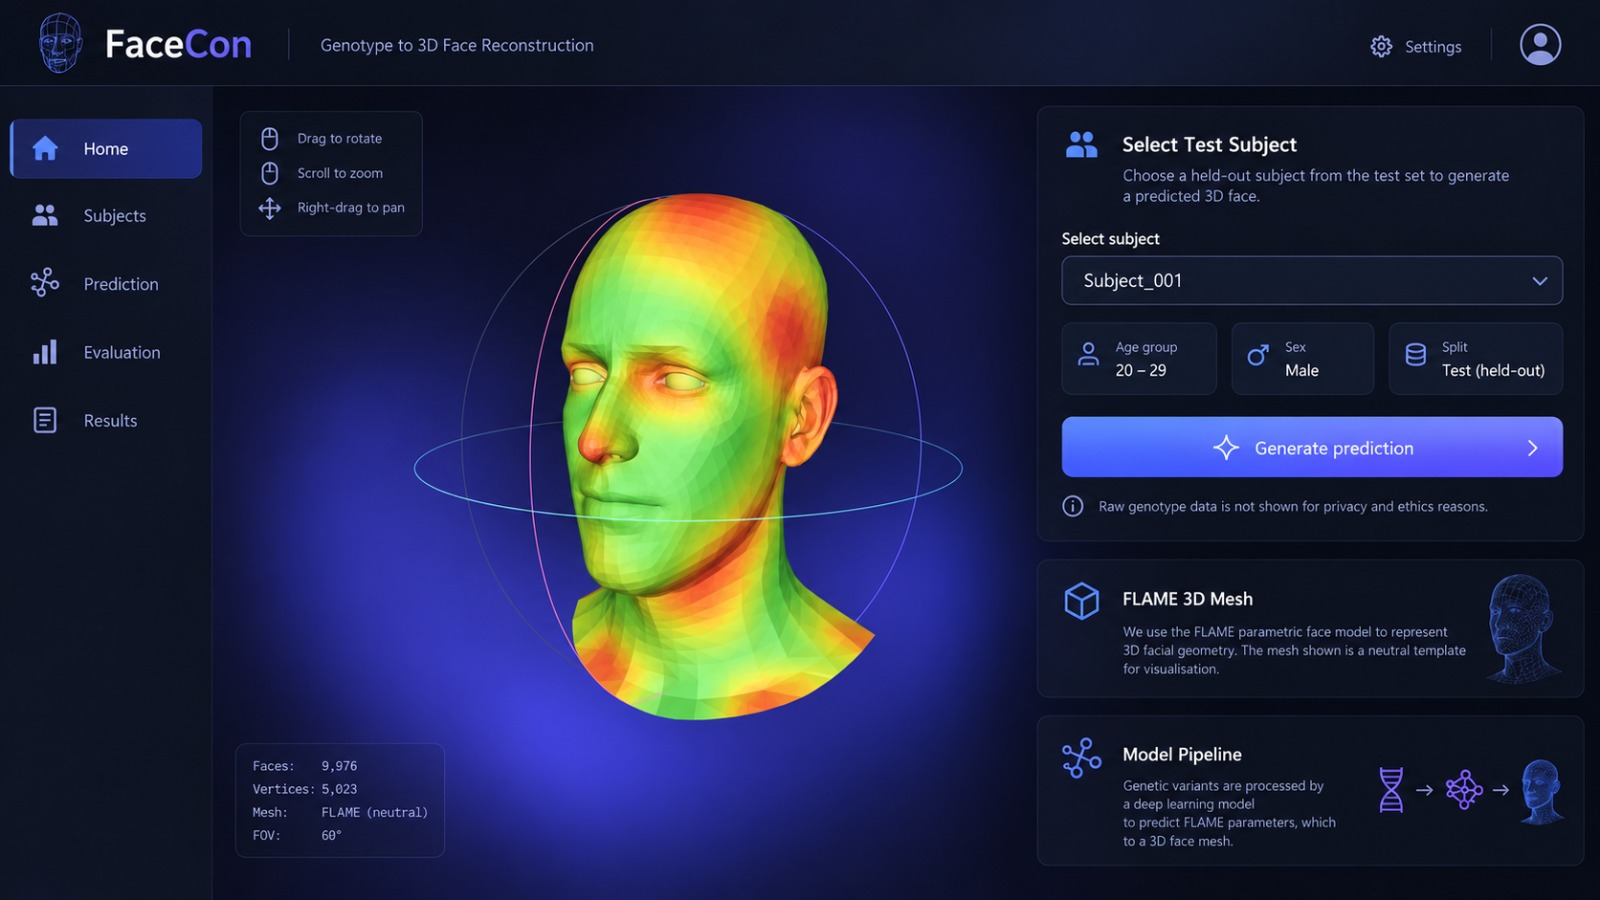
\includegraphics[width=\textwidth]{Figures/ui_selection.png}
\caption{Test subject selection screen (UC-04).}
\label{fig:ui1}
\end{figure}

\begin{figure}[!ht]
\centering
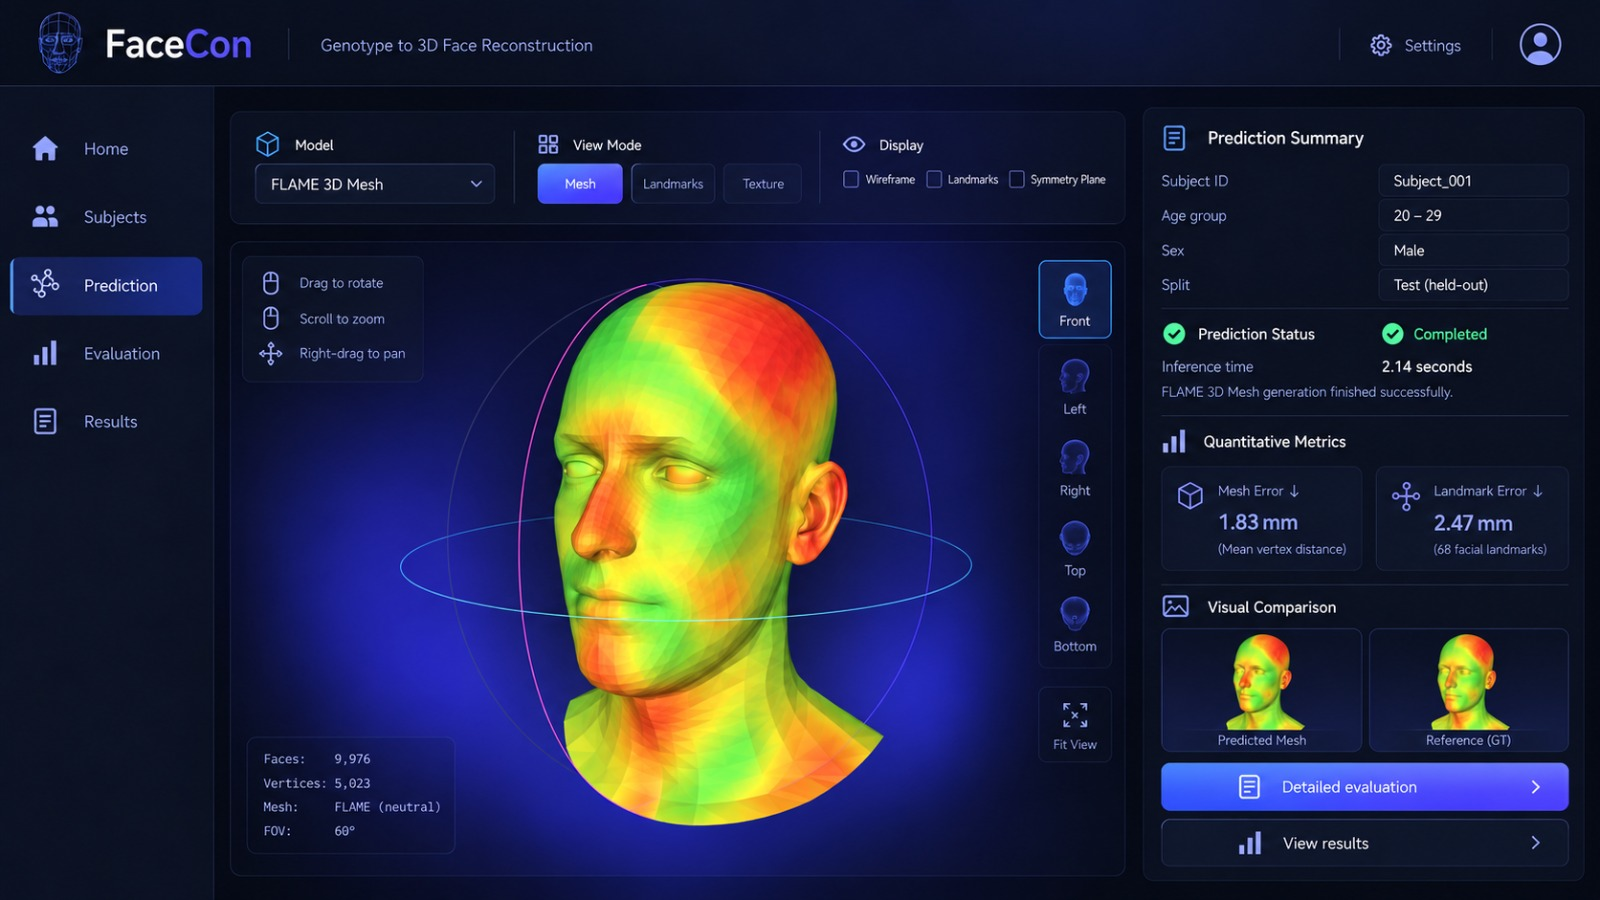
\includegraphics[width=\textwidth]{Figures/ui_comparison.png}
\caption{Prediction screen (UC-05).}
\label{fig:ui2}
\end{figure}

\begin{figure}[!ht]
\centering
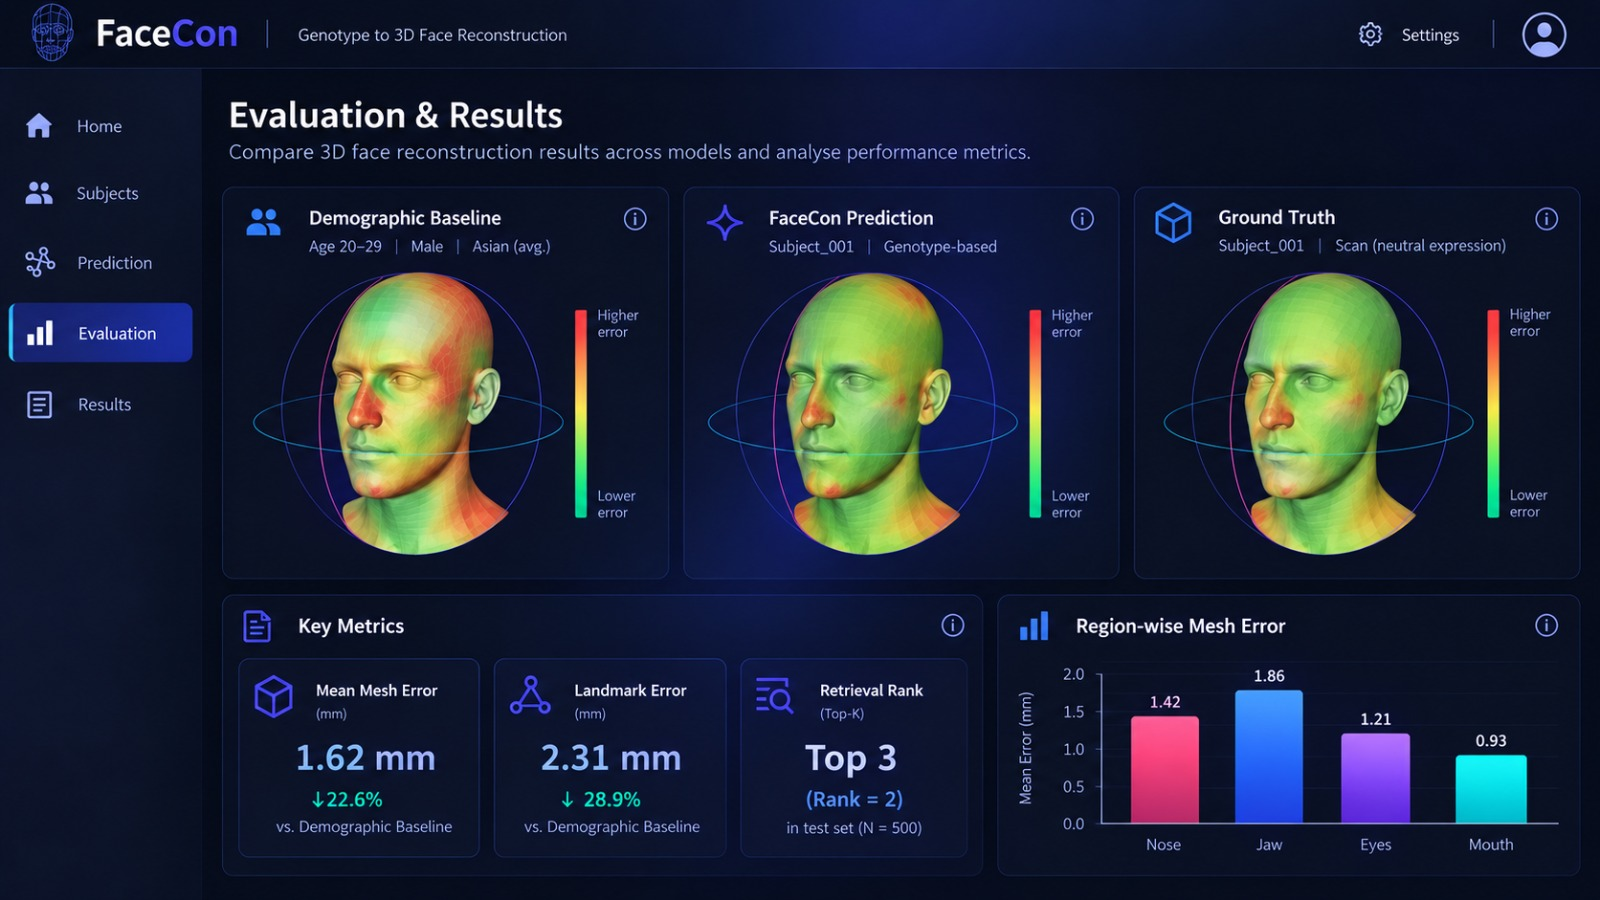
\includegraphics[width=\textwidth]{Figures/ui_detailed.png}
\caption{Evaluation and results screen (UC-06).}
\label{fig:ui3}
\end{figure}

\begin{figure}[!ht]
\centering
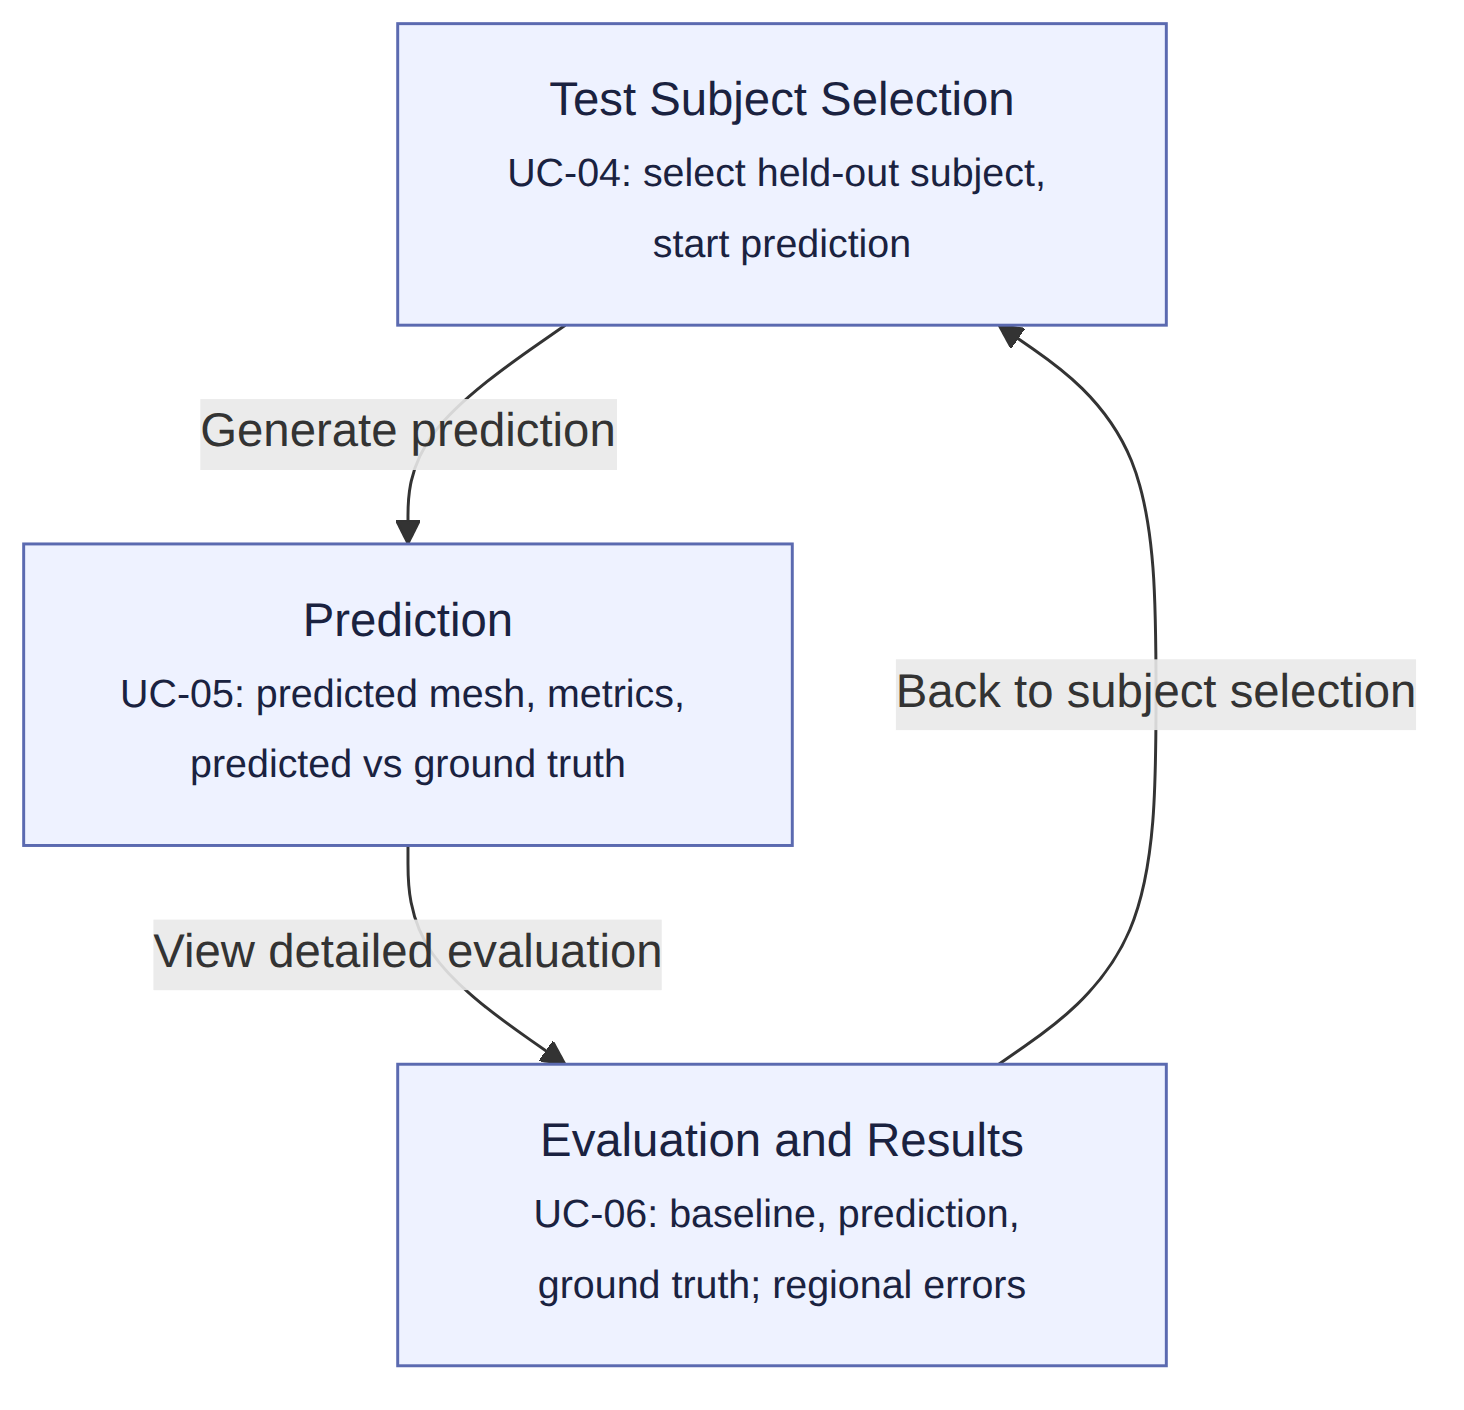
\includegraphics[width=0.5\textwidth]{Figures/nav.png}
\caption{Navigation flow of the demonstrator.}
\label{fig:nav}
\end{figure}

The mapping between the demonstrator screens and the use cases and functional requirements is as follows. Screen 1, test subject selection, realizes UC-04 and starts prediction through FR-06. Screen 2, prediction, realizes UC-05 and exercises FLAME decoding (FR-07) and evaluation (FR-08), presenting the predicted mesh, its metrics, and a comparison with the ground truth. Screen 3, evaluation and results, realizes UC-06 and exercises evaluation and baseline comparison (FR-08, FR-09), presenting the demographic baseline, the prediction, and the ground truth together with regional errors. Because the demonstrator displays a ground truth FLAME face alongside the prediction, it relies on the held-out FLAME targets produced by the registration stage (FR-04), which are available for evaluation but never used during training.

\section{Database Design}
FaceCon is data-centric rather than transaction-centric, so it stores structured, file artifacts rather than using a relational database. No SQL or entity-relationship schema is therefore required. The data design and dictionary are nonetheless documented.

\subsection{Data Dictionary}
Table~\ref{tab:datadict} is the data dictionary for the principal FaceCon artifacts, keyed by de-identified subject identifiers.

\begin{table}[!ht]
\centering
\caption{Data dictionary for the principal FaceCon data artifacts.}
\label{tab:datadict}
\small
\begin{tabular}{|P{2.6cm}|P{2.6cm}|P{2.2cm}|P{5.4cm}|}
\hline
\textbf{Entity} & \textbf{Field} & \textbf{Type} & \textbf{Description} \\ \hline
Subject & subject\_id & String & De-identified key linking genotype and scan. \\ \hline
Genotype & snp\_dosage & Int matrix & Allele dosages (0/1/2) for the documented SNP panel. \\ \hline
Genotype & qc\_flags & Struct & Per-subject QC outcomes and imputation notes. \\ \hline
FaceShape & flame\_params & Float array & FLAME identity/shape parameters from fitting. \\ \hline
FaceShape & fit\_error & Float & Registration error between scan and FLAME mesh. \\ \hline
Appearance & colour\_outputs & Categorical & Eye colour, hair colour, and skin colour returned by the integrated HIrisPlex-S predictor. \\ \hline
Appearance & hirisplex\_markers & Int matrix & Allele dosages for the HIrisPlex-S marker SNPs extracted from the genotype. \\ \hline
Demographics & age, gender, ancestry/PCs & Mixed & Covariates for baselines and stratification. \\ \hline
Split & split\_label & Enum & Train / validation / test assignment. \\ \hline
Prediction & pred\_params & Float array & Predicted FLAME shape for a subject. \\ \hline
Prediction & baseline\_params & Float array & Demographic-baseline FLAME shape for comparison. \\ \hline
\end{tabular}
\end{table}

\section{Risk Analysis}
This section identifies the main risks to the project, together with their category, cause, potential impact, likelihood, severity, and the mitigation and contingency measures planned for each. Because FaceCon is a research and development project that depends on controlled-access data and uncertain experimental outcomes, the most significant risks are concentrated in the data, methodological, and evaluation categories rather than in conventional software-failure categories. Table~\ref{tab:risk} summarizes the analysis.

{\footnotesize\setlength{\LTpre}{6pt}\setlength{\LTpost}{0pt}
\begin{longtable}{|P{2.5cm}|P{3.3cm}|P{2.5cm}|P{1.6cm}|P{3.0cm}|}
\caption{Risk analysis for the FaceCon project.}\label{tab:risk}\\
\hline
\textbf{Risk / Category} & \textbf{Description and Cause} & \textbf{Potential Impact} & \textbf{Likelihood / Severity} & \textbf{Mitigation and Contingency} \\ \hline
\endfirsthead
\hline
\textbf{Risk / Category} & \textbf{Description and Cause} & \textbf{Potential Impact} & \textbf{Likelihood / Severity} & \textbf{Mitigation and Contingency} \\ \hline
\endhead
\hline
\endfoot
Delayed or denied data access \newline (Access / Data) & Approval for dbGaP and FaceBase may be slow or refused, owing to institutional review and data-use-agreement processes. & Training on real data is blocked and the schedule may slip. & Medium / High & Develop and validate the pipeline on synthetic data in parallel. Contingency: continue methodological and synthetic-data work and escalate the access request. \\ \hline
Small usable paired-sample size \newline (Data / Methodological) & Few subjects may have both a genotype and a valid 3D scan after QC, because of scarcity and filtering. & Low statistical power and a tendency for complex models to overfit. & High / High & Prefer simple, regularized models and strong baselines, and report confidence intervals. Contingency: restrict scope to baselines and report limits honestly. \\ \hline
Poor scan to FLAME fitting \newline (Data quality / Preprocessing) & Some scans may register poorly to FLAME, owing to noise, missing regions, or landmark errors. & Label noise in training targets and biased evaluation. & Medium / Medium & Enforce fitting-error thresholds and exclude or flag poor fits. Contingency: correct landmarks manually or exclude the subject with documentation. \\ \hline
Demographic and population confounding \newline (Methodological / Evaluation) & Age, gender, and ancestry drive facial variation and can inflate apparent genotype accuracy. & Overstated individual-level genetic contribution. & High / Medium & Evaluate demographic-only, genotype-only, and combined models and report the incremental gain. Contingency: stratified analysis and explicit reporting of confounding. \\ \hline
Data leakage across splits \newline (Methodological / Evaluation) & Subjects or fitted statistics could leak between splits through relatedness or statistics fitted on all data. & Optimistic, irreproducible results. & Medium / High & Use subject-level splits that respect relatedness and fit statistics on training folds only. Contingency: re-run with corrected splits and discard affected results. \\ \hline
Overfitting of complex models \newline (Modelling) & High-dimensional SNP inputs relative to a small sample encourage memorization. & Misleadingly low training error and poor generalization. & Medium / Medium & Follow the baselines first progression with regularization and early stopping, matching complexity to the data. Contingency: fall back to simpler models. \\ \hline
Ancestry bias and limited generalization \newline (Research / Data) & GWAS priors and the cohort are skewed toward specific ancestries. & Results may not transfer to other populations. & Medium / Medium & Document provenance and stratify by ancestry where possible. Contingency: scope conclusions to the evaluated population. \\ \hline
Integration and reproducibility drift \newline (Integration / Reproducibility) & Dependency, seed, or configuration changes across environments. & Non-reproducible results and wasted effort. & Low / Medium & Pin dependencies, fix seeds, and capture per-run configurations. Contingency: restore the exact recorded configuration. \\ \hline
Schedule compression \newline (Schedule) & Research uncertainty and data delays reduce the available time. & Incomplete experiments by the deadline. & Medium / Medium & Prioritize baselines and core evaluation and treat advanced models as stretch goals. Contingency: descope the advanced generative stage. \\ \hline
\end{longtable}
}

\section{Conclusion}
This chapter has specified what FaceCon must do and how well it must do it. The features were turned into functional requirements written in a testable form, so that each can be traced to a test case in Chapter~\ref{ch:impl}, and the non-functional requirements fixed the properties that matter most for a research system of this kind: reproducibility, protection of controlled-access data, and the separation of training data from everything used to judge a model. The use cases describe how a user selects a held-out subject, generates a prediction, and compares it with the demographic baseline and the ground truth, and the interface designs give those use cases a concrete form. The data design records the artefacts the pipeline produces in a data dictionary rather than a relational schema, since FaceCon stores structured files and not transactions. The risk analysis anticipated the most serious problem the project met, the delay in data access, and its mitigation, a simulated cohort, is what made the rest of this phase possible. The next chapter develops the methodology that meets these requirements.

\chapter{Proposed Approach and Methodology}
\label{ch:method}
This chapter describes the proposed approach and methodology for FaceCon as a procedural and algorithmic framework rather than as code. It follows the data end-to-end: acquiring and cleaning genotypes, constructing a documented SNP panel, registering scans to FLAME, pairing the modalities, and then training a disciplined progression of models and evaluating them against baselines. The guiding principle is that every step is documented and reproducible, and that the evaluation is designed to separate genuine genetic signal from demographic confounding. Figure~\ref{fig:pipeline} shows the end-to-end pipeline.

\begin{figure}[!h]
\centering
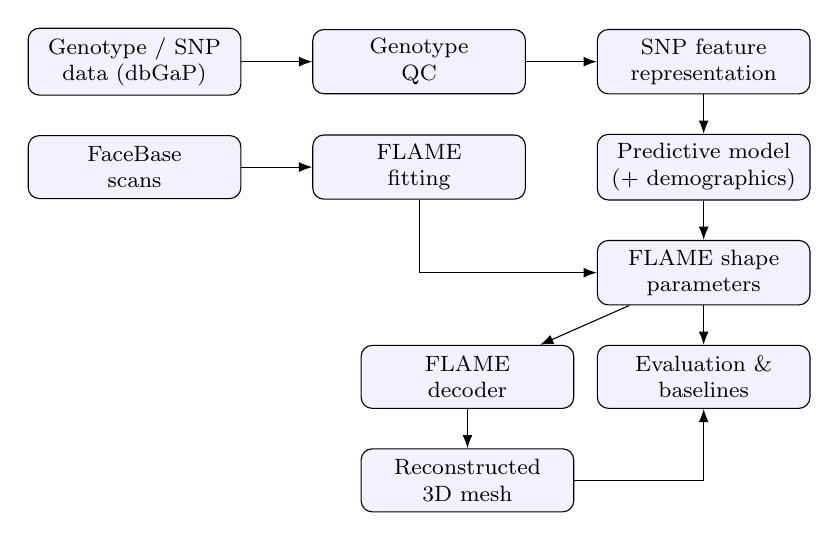
\begin{tikzpicture}[node distance=0.5cm and 0.9cm,every node/.style={font=\footnotesize}]
\tikzstyle{st}=[draw,rounded corners,fill=blue!5,minimum width=2.7cm,minimum height=0.8cm,align=center]
\node[st](a){Genotype / SNP\\data (dbGaP)};
\node[st,right=of a](b){Genotype\\QC};
\node[st,right=of b](c){SNP feature\\representation};
\node[st,below=of c](d){Predictive model\\(+ demographics)};
\node[st,below=of a,xshift=0cm](s){FaceBase\\scans};
\node[st,right=of s](f){FLAME\\fitting};
\node[st,below=of d](e){FLAME shape\\parameters};
\node[st,below=of e,xshift=-3.0cm](g){FLAME\\decoder};
\node[st,below=of e,xshift=0cm](h){Evaluation \&\\baselines};
\node[st,below=of g](m){Reconstructed\\3D mesh};
\draw[-{Latex}](a)--(b);\draw[-{Latex}](b)--(c);\draw[-{Latex}](c)--(d);
\draw[-{Latex}](s)--(f);\draw[-{Latex}](f)|-(e);
\draw[-{Latex}](d)--(e);\draw[-{Latex}](e)--(g);\draw[-{Latex}](e)--(h);
\draw[-{Latex}](g)--(m);\draw[-{Latex}](m)-|(h);
\end{tikzpicture}
\caption{FaceCon end-to-end methodology.}
\label{fig:pipeline}
\end{figure}

\section{Dataset}
FaceCon uses 3DFN subjects who have both genotype data from dbGaP (accession phs000949)~\cite{ref:dbgap} and 3D facial scans and related phenotype resources from FaceBase~\cite{ref:facebase}. After controlled access is granted, we will inspect file formats, missingness, demographics, scan quality, and subject-identifier overlap before fixing the final model capacity, because the usable paired sample count is not known in advance and directly determines how complex a model is justified.

Controlled access to these data was still pending when the prototype was built. As an interim measure, the pipeline was therefore developed and validated on a simulated cohort whose size, covariates, and measurement set follow the public description of the 3DFN GWAS~\cite{ref:shaffer,ref:weinberg}, and which carries published association signals. The simulated cohort is described in Chapter~\ref{ch:impl} and the results obtained on it in Chapter~\ref{ch:results}. It replaces neither the dataset described above nor any step of this methodology, and every statement in this chapter about real data describes work still to be done once access is granted.

\section{Genotype Preprocessing and SNP Selection}
Genotypes are processed with a standard genome analysis toolkit~\cite{ref:plink}. The preprocessing pipeline comprises subject- and SNP-level missingness filtering, minor-allele-frequency filtering, Hardy--Weinberg filtering where appropriate, imputation or documented missing-value handling, optional linkage-disequilibrium pruning, SNP standardization, and optional ancestry or PC covariates. Every threshold and decision is recorded so the input to modeling can be reconstructed.

SNP selection is fully documented, recording for each SNP its identifier, chromosome, position, locus, facial-trait association, source paper, and reason for inclusion. FaceCon does not blindly copy Difface's 7,842-SNP panel. To answer RQ4, the methodology compares three panel constructions: (1) facial-GWAS-informed SNPs~\cite{ref:white,ref:xiong,ref:claes}; (2) matched random or common SNPs as a control; and (3) larger QC-filtered panels if sample size allows. Each subject's genotype is encoded as an allele-dosage vector with entries in $\{0,1,2\}$ (homozygous reference, heterozygous, homozygous alternate), giving the conceptual tensor $X_{\mathrm{snp}} \in \mathbb{R}^{\,n_{\mathrm{subjects}} \times n_{\mathrm{snps}}}$, with demographic covariates in $X_{\mathrm{demo}}$.

\section{Face Preprocessing with FLAME}
FaceBase scans are standardized through FLAME~\cite{ref:flame} so that every subject shares one mesh topology. The procedure normalizes and aligns each scan, initializes landmarks, fits or registers FLAME to the scan, and exports the FLAME identity/shape coefficients as the standardized training target $Y_{\mathrm{face}}$. Concretely, fitting minimizes a weighted landmark and surface objective over the FLAME shape $\beta$, pose $\theta$, and expression $\psi$:
\begin{equation}\label{eq:fit}
\min_{\beta,\theta,\psi}\; \lambda_{\mathrm{lmk}}\!\sum_{k}\lVert \pi(v_k(\beta,\theta,\psi)) - u_k\rVert_2^2 \;+\; \lambda_{\mathrm{surf}}\!\sum_{p\in S}\min_{q\in M}\lVert p-q\rVert_2^2 \;+\; \lambda_{\mathrm{reg}}\lVert\beta\rVert_2^2 .
\end{equation}

Equation~\ref{eq:fit} is the registration, or fitting, objective. It is used in the face preprocessing stage, where it converts each raw FaceBase scan into a face expressed in the common FLAME representation. It is needed because the raw scans do not share a common topology and therefore cannot be compared across subjects or used as a learning target directly. Minimising the objective finds the FLAME parameters whose resulting mesh best matches the scan, after which the identity component of those parameters becomes the training target.

The symbols in Equation~\ref{eq:fit} are defined as follows. The optimisation variables are the FLAME shape, or identity, parameters $\beta$, the pose parameters $\theta$, and the expression parameters $\psi$, which together determine a FLAME mesh. The function $v_k(\beta,\theta,\psi)$ returns the position of the $k$th FLAME landmark vertex for the current parameters, and $\pi(\cdot)$ projects that three-dimensional position so that it can be compared with the detected landmark $u_k$ on the scan. The term $S$ is the set of points on the scan surface, $M=M(\beta,\theta,\psi)$ is the FLAME mesh surface for the current parameters, and $q$ is the point on $M$ that is closest to a scan point $p$. The notation $\lVert\cdot\rVert_2$ denotes the Euclidean distance. The weights $\lambda_{\mathrm{lmk}}$, $\lambda_{\mathrm{surf}}$, and $\lambda_{\mathrm{reg}}$ balance the three terms of the objective.

The objective has three parts. The first term is the landmark term, which pulls the FLAME landmarks towards the detected landmarks on the scan and provides a stable, coarse alignment. The second term is the surface term, which measures how far the FLAME mesh surface lies from the scan surface and refines the fit over the whole face. The third term is a regularisation term on $\beta$, which keeps the shape within the plausible range learned by the FLAME model and prevents the fit from overfitting to scan noise. Only the identity parameters $\beta$ are retained as the prediction target $Y_{\mathrm{face}}$, because pose and expression are nuisance factors for genotype prediction, and the FLAME decoder reconstructs the mesh vertices from $\beta$ when a geometric evaluation is required.

\section{Modelling Strategy}
The modelling strategy follows a baselines first progression, where simpler and more interpretable models are evaluated before increasingly complex architectures. This allows the contribution of additional model complexity to be measured directly. FaceCon takes architectural inspiration from Difface's two-stage alignment and generation framework~\cite{ref:difface}, while adapting the implementation to the 3DFN dataset and FLAME representation. The planned progression is as follows.
\begin{enumerate}
\item The mean-face baseline predicts the training-set mean shape for every subject and ignores all inputs. It is the floor that any informative model must beat, and it quantifies how much apparent accuracy comes simply from predicting an average face.
\item The demographic regression is a linear model that predicts FLAME shape from demographic covariates alone, namely age, sex, and ancestry PCs. It measures how much of the face is explained by demographics before any genetic information is used, and is a mandatory baseline for separating genetic signal from population structure.
\item Ridge regression on the SNP panel is a regularised linear model that maps SNP dosages to FLAME parameters, where the L2 penalty controls overfitting when the number of SNPs is large relative to the sample size. It provides an interpretable, sample-efficient first genetic model.
\item An MLP on the SNP panel is a feed-forward neural network that learns non-linear relationships between the SNP inputs and the FLAME shape coefficients, testing whether non-linear structure improves on ridge regression.
\item An MLP on SNPs combined with demographic covariates is the same network with the covariates concatenated to the SNP input, so that the genetic contribution can be measured on top of, rather than confounded with, demographics.
\item Extended MLP architectures are deeper or wider networks with additional regularisation such as dropout and weight decay, explored only if the base MLP shows learnable signal, to probe whether added capacity yields real improvement.
\item A Transformer-based SNP encoder~\cite{ref:transformer} uses self-attention, with suitable SNP embeddings and genomic positional information, to model interactions across SNPs and produce a learned genetic representation that is then decoded to FLAME parameters.
\item Contrastive SNP--face representation learning~\cite{ref:clip} aligns genetic and facial embeddings in a shared space, pulling matched genotype--face pairs together and pushing mismatched pairs apart, so that a face-predictive representation can be learned from paired data.
\item A generative or diffusion model~\cite{ref:ddpm,ref:ldm} maps a genetic representation to a facial representation using a generative or diffusion prior before FLAME decoding, capturing the distribution of plausible faces; used only where the final dataset and preceding experiments support its added complexity.
\end{enumerate}
The first complete neural pipeline maps an SNP vector through an MLP to FLAME shape coefficients, which are then decoded into a 3D facial mesh. The advanced modelling stage extends this approach using transformer SNP representations and contrastive learning between genetic and facial features. A further generative stage may map SNP representations to facial representations before FLAME decoding, including the use of a diffusion prior if supported by the available data. All architectures will be evaluated using the same data splits and evaluation framework. This allows FaceCon to determine whether increasingly complex models provide meaningful improvements over simpler statistical and neural baselines.

\section{Appearance Integration via HIrisPlex-S}
In addition to three-dimensional shape, FaceCon provides a set of externally visible colour attributes, namely eye colour, hair colour, and skin colour. FaceCon does not train a new model for these colours. Instead, it integrates HIrisPlex-S~\cite{ref:hirisplex,ref:hirisplexs}, the established forensic DNA phenotyping method that is the de facto standard for predicting eye, hair, and skin colour from a small, validated marker panel. The appearance component is therefore an integration, not a trained classifier: the same dbGaP genotype that drives shape prediction is reused as the input.

The integration has a simple, fixed flow. From the subject's genotype, FaceCon extracts the HIrisPlex-S marker SNPs; these markers are passed to the established HIrisPlex-S predictor as published; and the predictor returns eye colour, hair colour, and skin colour, which are then passed to the visualization layer. Because HIrisPlex-S is an existing, externally validated forensic method, FaceCon uses it directly and does not retrain, re-fit, or re-calibrate it, and it does not construct a pigmentation panel of its own. This keeps the two branches cleanly separated: the shape branch runs dbGaP genotype through facial SNP selection and the FaceCon shape models to FLAME parameters and a predicted 3D mesh, while the appearance branch runs the same dbGaP genotype through HIrisPlex-S marker extraction and the HIrisPlex-S predictor to eye, hair, and skin colour.

The predicted colours are reported using HIrisPlex-S as published, with its own documented and externally validated performance rather than any accuracy derived on the project's own data. Skin colour and eye colour are rendered on the reconstructed face, and hair colour is reported, and rendered only where suitable hair geometry exists. FaceCon does not claim that the 3DFN resource provides ground-truth eye, hair, or skin colour labels, and therefore does not train or evaluate an appearance classifier against such labels; the appearance output is the integrated forensic prediction, shown alongside the reconstructed shape.

In the current prototype the HIrisPlex-S model is evaluated by a local module, described together with its limitations in Chapter~\ref{ch:impl}. The module reproduces the behaviour of the official calculator and fits nothing itself, so FaceCon makes no claim about the accuracy of the colour predictions beyond what the published validation of HIrisPlex-S reports.

\section{Research Questions}
The methodology is organized to answer the research questions of Chapter~\ref{ch:intro}. RQ1 is answered by the construction of the reproducible pipeline itself. RQ2 and RQ3, which concern the accuracy of SNP prediction relative to and in addition to demographics, are answered by the baseline comparisons. RQ4 is answered by the GWAS-informed versus matched-random SNP-panel ablation, and RQ5 by the progression from simple statistical models to more complex neural architectures. RQ6 is answered by the region-level analysis of which facial areas carry the strongest predictable signal. RQ7 is answered by stratified evaluation across demographic and ancestry subgroups, carried out where the final dataset contains enough samples for a statistically meaningful comparison. Finally, RQ8 is answered by the integration of the established HIrisPlex-S forensic method with the shape pipeline, so that eye, hair, and skin colour are obtained from the same genotype and shown alongside the reconstructed face.

\section{Evaluation}
Evaluation is built before any final model claims and spans the following complementary measures.
\begin{enumerate}
\item FLAME parameter error is measured as MSE, RMSE, MAE, and the per-component correlation between predicted and true coefficients.
\item Mesh error is the per-vertex Euclidean distance, reported as mean and median vertex error.
\item Landmark error is the distance between predicted and true positions at anatomical landmarks.
\item Region analysis breaks the error down by nose, jaw, mouth, eyes, cheeks, forehead, and whole face.
\item Retrieval-style ranking reports the Top-1, Top-5, and mean rank of the true face among candidates, as a scientific metric only and not as forensic identification.
\item Baseline comparisons set every model against the mean-face, demographics-only, SNP-only, and SNP+demographics predictors.
\item Ablations cover GWAS versus random SNPs, panel size, removal of demographics, and architecture comparison.
\item Appearance colour is obtained from the integrated HIrisPlex-S predictor and described using its published, externally validated performance. It is not re-evaluated on 3DFN, which does not provide eye, hair, or skin colour labels, and Section~\ref{sec:res-appearance-untested} explains why no other cohort could be used either.
\end{enumerate}
Small gains are interpreted honestly: for example, if demographics alone achieve a mean vertex error of 4.2~mm and SNP+demographics achieve 4.18~mm, the methodology reports that SNPs added little individual-level signal under that setup rather than presenting the model as a success.

\section{Experimental Integrity}
Several rules protect the validity of the results. Splits are strictly subject-level, so no subject (or close relative) appears in more than one split. No test data leaks into SNP discovery, PC estimation, or normalization: external GWAS SNP lists are cited and fixed in advance, and any within-dataset SNP selection is performed only inside training folds. Reporting always separates genetic, demographic, and ancestry contributions. Finally, the discussion addresses privacy, misuse risk, ancestry bias, and the genuine uncertainty of individual-level accuracy, consistent with the project's commitment not to claim that DNA uniquely reconstructs a person's exact face.

\section{Conclusion}
This chapter has presented the methodology as a documented pipeline that runs from dbGaP genotypes and FaceBase scans to an evaluated model, with every step chosen so that it can be repeated and checked. The modelling strategy is a baselines-first progression, in which each more complex model must show that it improves on a simpler one under identical data splits and identical evaluation, so that added complexity is justified by results rather than assumed. The evaluation measures error on the shape parameters, on the decoded mesh, at landmarks, and by facial region, and always against the demographic baseline, because the question the project asks is what genotype adds beyond demographics. The integrity rules forbid any leakage of test subjects into SNP selection, normalisation, or model selection, and they require genetic, demographic, and ancestry contributions to be reported separately. Colour is provided by integrating the HIrisPlex-S method rather than training a new model. Each research question was mapped to the analysis that answers it. The next chapter presents the design that realises this methodology in software.

\chapter{High-Level and Low-Level Design}
\label{ch:design}
This chapter presents the design of FaceCon, from the overall architecture down to the classes, modules, and interface contracts that implement it. The design realizes the methodology of the previous chapter and keeps the pipeline stages modular, so that any stage can be developed, tested, or replaced independently and so that simple and complex models share common data and decode interfaces. Throughout the chapter it is important to keep three ideas distinct: the system (software) architecture, which is how the code and its components are organized; the machine-learning model architecture, which is the internal structure of a particular predictor such as an MLP or a transformer; and the modelling strategy, which is the baselines first progression described in Chapter~\ref{ch:method}. This chapter concerns the first of these, and refers to the other two only where the software must accommodate them.

\section{System Overview}
FaceCon is a layered, modular system. A thin interface layer exposes configuration-driven tools for the researcher-developer and evaluator, together with a lightweight local web demonstrator. Beneath it, a processing layer contains the pipeline modules for genotype QC and SNP selection, scan to FLAME fitting, subject matching and splitting, model training, and evaluation. A model layer holds the interchangeable shape predictors (mean-face, demographic, ridge, MLP, and optional advanced models) together with the shared FLAME decoder, and a parallel appearance component that integrates the established HIrisPlex-S predictor and renders its eye, hair, and skin colour outputs onto the decoded face. A data layer persists genotypes, registered meshes, FLAME parameters, splits, checkpoints, and results. This separation lets the scientific logic, the model definitions, and the storage evolve independently, and it keeps the demonstrator a thin client over the trained shape models and the integrated appearance predictor.

\section{Design Considerations}
This section records the assumptions, constraints, and guiding goals that shape the design before the architecture is presented, together with the development method followed. They are stated first because they explain choices that might otherwise look arbitrary, such as why the system stores files rather than a database, why every model sits behind one interface, and why the simplest adequate model is always preferred.

\subsection{Assumptions and Dependencies}
FaceCon assumes access to the required FLAME model files, genotype-processing tools, deep learning libraries, and 3D mesh utilities. It also depends on approved access to the 3DFN genotype and facial data, which must be stored and processed according to the applicable data-use agreement. The system assumes a consistent FLAME topology for facial representation. The main pipeline is intended for technical users, while the final demonstrator is designed so that evaluators can view and compare predictions without needing knowledge of the underlying implementation.

\subsection{General Constraints}
The design must respect privacy constraints, so that no raw individual-level data appears in released artifacts. It must satisfy reproducibility constraints, so that all runs are configuration- and seed-driven, and scientific constraints, so that splits are strictly subject-level with no leakage. It must also avoid machine-specific hard-coded paths, a defect explicitly identified in prior work.

\subsection{Goals and Guidelines}
The design follows the ``keep it simple'' principle. The smallest model that fits the data is preferred, because the paired-sample size is modest and over-large models would overfit and obscure the scientific question. Clarity and reproducibility are valued over architectural novelty.

\subsection{Development Methods}
Development is incremental. Each module is built and unit-tested against synthetic data first, so the full pipeline is runnable end-to-end before real data access is finalized, and it is then validated on real data as that data becomes available. Interchangeable data loaders for synthetic and real data share one interface, so that experiments can be developed before approval completes.

\section{System Architecture}
Figure~\ref{fig:arch} shows the layered architecture. Control flows downward from the interface layer, which issues configuration-driven commands. The processing layer orchestrates the pipeline, the model layer performs training and inference, and the data layer persists every artifact. The rationale for this decomposition is that the expensive, one-time data preparation is cleanly separated from the frequently-repeated model experimentation, and that a shared decode and evaluation interface lets every model, from mean-face to advanced, be compared on equal terms.

\begin{figure}[!ht]
\centering
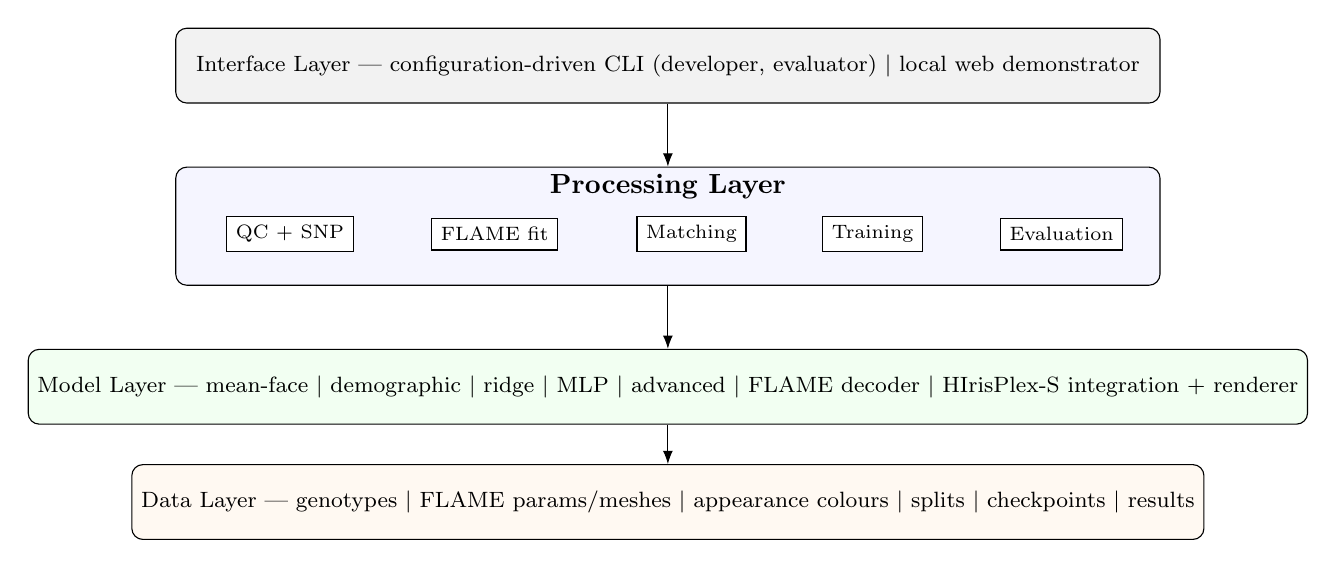
\begin{tikzpicture}[node distance=0.5cm,every node/.style={font=\footnotesize}]
\tikzstyle{lay}=[draw,rounded corners,minimum width=12.5cm,minimum height=0.95cm,align=center]
\node[lay,fill=gray!10](i){Interface Layer --- configuration-driven CLI (developer, evaluator) $\vert$ local web demonstrator};
\node[lay,below=0.8cm of i,fill=blue!4,minimum height=1.5cm](p){};
\node[font=\bfseries] at ([yshift=0.5cm]p.center){Processing Layer};
\node[draw,fill=white,font=\scriptsize] at ([yshift=-0.1cm,xshift=-4.8cm]p.center){QC + SNP};
\node[draw,fill=white,font=\scriptsize] at ([yshift=-0.1cm,xshift=-2.2cm]p.center){FLAME fit};
\node[draw,fill=white,font=\scriptsize] at ([yshift=-0.1cm,xshift=0.3cm]p.center){Matching};
\node[draw,fill=white,font=\scriptsize] at ([yshift=-0.1cm,xshift=2.6cm]p.center){Training};
\node[draw,fill=white,font=\scriptsize] at ([yshift=-0.1cm,xshift=5.0cm]p.center){Evaluation};
\node[lay,below=0.8cm of p,fill=green!5](m){Model Layer --- mean-face $\vert$ demographic $\vert$ ridge $\vert$ MLP $\vert$ advanced $\vert$ FLAME decoder $\vert$ HIrisPlex-S integration + renderer};
\node[lay,below=0.5cm of m,fill=orange!5](d){Data Layer --- genotypes $\vert$ FLAME params/meshes $\vert$ appearance colours $\vert$ splits $\vert$ checkpoints $\vert$ results};
\draw[-{Latex}](i)--(p);\draw[-{Latex}](p)--(m);\draw[-{Latex}](m)--(d);
\end{tikzpicture}
\caption{Layered system architecture of FaceCon.}
\label{fig:arch}
\end{figure}

\subsection{Subsystem Architecture}
The processing layer is decomposed into two loosely-coupled subsystems that share the data layer. The data-preparation subsystem, which performs QC, SNP selection, FLAME fitting, subject matching, and splitting, is deterministic and runs once per data release to produce the paired dataset and fixed splits. The learning and evaluation subsystem, which contains the models, the FLAME decoder, the metrics, the baselines, and the ablations, is run many times during experimentation. Separating them ensures that the costly preparation is not repeated during model iteration and that either subsystem can be tested in isolation against fixed artifacts. The codebase organization mirrors this decomposition, with top-level packages for \texttt{data}, \texttt{preprocessing}, \texttt{flame}, \texttt{models}, \texttt{appearance}, \texttt{training}, \texttt{evaluation}, \texttt{experiments}, and \texttt{configs}. The \texttt{appearance} package holds the HIrisPlex-S marker extraction, the integration wrapper around the external HIrisPlex-S predictor, and the renderer; it reuses the same genotype loaders as the shape pipeline but trains no model of its own.

\section{Architectural Strategies}
This section evaluates the main software-architecture strategies that were considered for FaceCon and states which were adopted. These are decisions about how the system is structured, and they are distinct from the choice of machine-learning model architecture and from the modelling strategy, both of which belong to Chapter~\ref{ch:method}.

\subsection{Monolithic Script}
A monolithic design would place preprocessing, modelling, and evaluation in a single script or notebook. It is quick to start and needs no interface design. However, it tightly couples unrelated concerns, makes reproducibility and testing difficult, and would force the expensive data preparation to be repeated on every run. For a project that must run many model experiments on fixed data, this approach was judged inappropriate.

\subsection{Layered Modular Pipeline}
A layered modular pipeline separates the system into interface, processing, model, and data layers, with the processing layer further split into data-preparation and learning and evaluation subsystems. Applied to FaceCon, this lets data preparation run once and model experiments run repeatedly against the stored artifacts. Its advantages are testability, reproducibility, and clear separation of concerns. Its trade-off is the up-front effort of defining module boundaries and interfaces. Given the project's emphasis on reproducibility and repeated experimentation, this approach is appropriate and was adopted.

\subsection{Interface Interchangeable Models}
In this strategy every predictor, from the mean-face baseline to an advanced model, implements a common interface, so that training and evaluation code is model-agnostic. Applied to FaceCon, it allows the baselines first progression and the ablations to be run by changing configuration rather than rewriting code. Its advantage is that every model is compared on identical data and metrics, which is essential for honest comparison. Its trade-off is that the interface must be general enough to cover both statistical and neural models. This strategy is appropriate for the project and was adopted.

\subsection{Shared Representation Contract}
A further strategy is to require every model to predict the same quantity, namely FLAME shape coefficients, and to decode predictions through a single shared FLAME-decode component. Applied to FaceCon, this turns a difficult high-dimensional geometry problem into a compact, well-defined regression target and guarantees that all models are directly comparable. Its advantage is simplicity and comparability. Its trade-off is a ceiling on fine geometric detail, which is acceptable given the project's scope. The alternative of predicting raw mesh vertices was rejected as high-dimensional and lacking cross-subject correspondence. This strategy was adopted.

\subsection{Service Architecture}
A service or microservice architecture would expose preprocessing, modelling, and evaluation as separate networked services. This can aid scaling and independent deployment. For a single-team research project with a modest dataset and no production-scale or multi-tenant requirement, the operational overhead outweighs the benefit, so this approach was considered but not adopted.

\subsection{Selected Approach}
FaceCon adopts a layered modular pipeline in which models are interchangeable behind a common interface and all of them honour a shared FLAME representation contract decoded by a single component. This combination directly serves the project's priorities of reproducibility, honest and like-for-like model comparison, and manageable complexity, while leaving room to add advanced models without disturbing the pipeline.

\section{Domain Model / Class Diagram}
Figure~\ref{fig:class} shows the principal classes of FaceCon, their key responsibilities, and their relationships. The diagram distinguishes three relationship types: solid lines for associations (one class uses another), dashed arrows for dependencies (one class consumes another's output or type), and hollow-triangle arrows for inheritance (a concrete class realizes an interface). It covers both the research pipeline and the demonstrator. Table~\ref{tab:models} then lists the model inventory that the \texttt{Model} interface makes interchangeable.

\begin{sidewaysfigure}
\centering
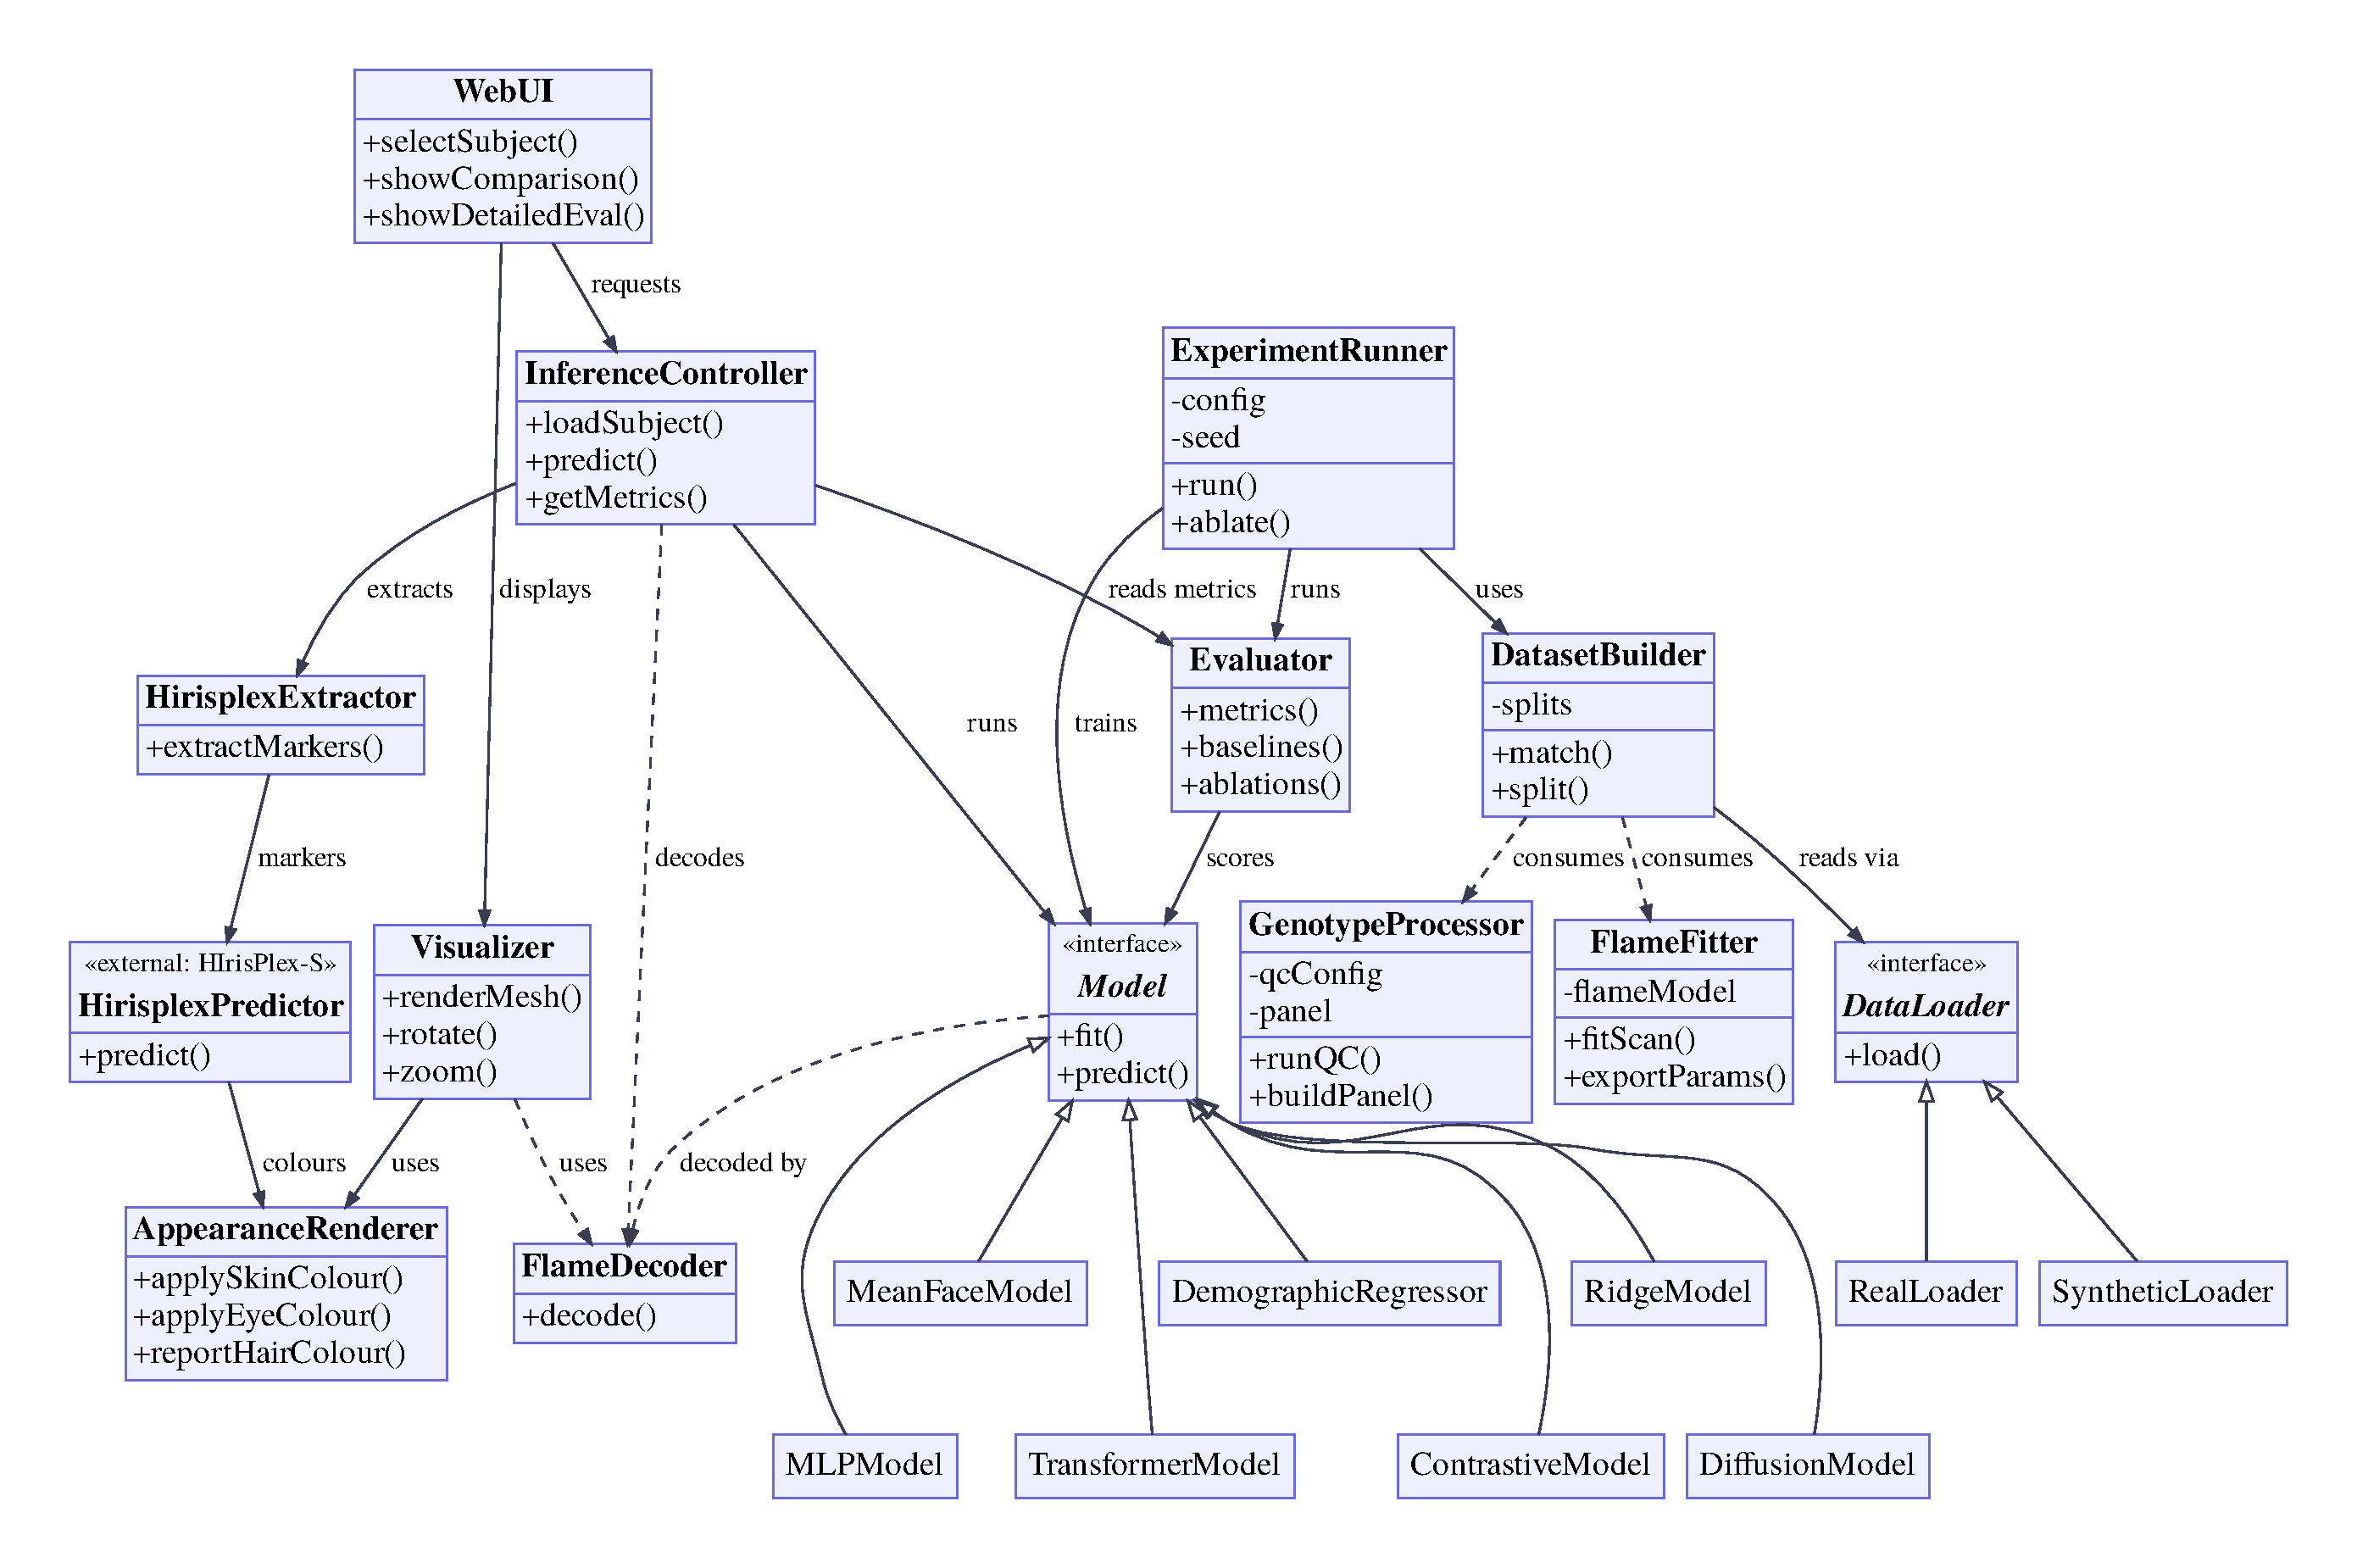
\includegraphics[width=0.98\textheight,height=0.86\textwidth,keepaspectratio]{Figures/class_diagram.pdf}
\caption{Class diagram of FaceCon.}
\label{fig:class}
\end{sidewaysfigure}

The diagram reflects the architecture directly. On the research side, \texttt{ExperimentRunner} is the orchestrator and is associated with \texttt{DatasetBuilder}, the \texttt{Model} interface, and \texttt{Evaluator}. \texttt{DatasetBuilder} depends on the outputs of \texttt{GenotypeProcessor} and \texttt{FlameFitter} and reads data through the \texttt{DataLoader} interface, which is realized by \texttt{SyntheticLoader} and \texttt{RealLoader} so that synthetic and real data are interchangeable. Every concrete predictor, from \texttt{MeanFaceModel} and \texttt{DemographicRegressor} through \texttt{RidgeModel}, \texttt{MLPModel}, and \texttt{TransformerModel}, realizes the single \texttt{Model} interface and is therefore interchangeable. Each model's predicted FLAME parameters are decoded by the shared \texttt{FlameDecoder}, and \texttt{Evaluator} computes metrics and baselines over the decoded meshes and the predicted parameters. The appearance component is a thin integration rather than a trained model: \texttt{HirisplexExtractor} selects the HIrisPlex-S marker SNPs from the same genotype, and \texttt{HirisplexPredictor} wraps the external, already-validated HIrisPlex-S method to return eye, hair, and skin colour; \texttt{AppearanceRenderer} then applies the predicted skin colour and eye colour to the decoded mesh and reports hair colour, rendering it only where suitable hair geometry exists. No appearance model is trained or scored by \texttt{Evaluator}. On the demonstrator side, \texttt{WebUI} requests predictions from \texttt{InferenceController}, which runs the trained \texttt{Model} and the integrated \texttt{HirisplexPredictor}, decodes the result through \texttt{FlameDecoder}, colours it through \texttt{AppearanceRenderer}, and reads metrics from \texttt{Evaluator}, while \texttt{Visualizer} renders the resulting faces in the interface. These demonstrator classes are the software counterparts of the interactions shown in the sequence diagrams of Section~\ref{sec:seq}.

\begin{table}[!ht]
\centering
\caption{Model inventory, all realizing the common Model interface and shared FLAME-decode contract.}
\label{tab:models}
\small
\begin{tabular}{|P{3.6cm}|P{3.2cm}|P{2.4cm}|P{3.0cm}|}
\hline
\textbf{Model} & \textbf{Input} & \textbf{Output} & \textbf{Role} \\ \hline
Mean face & --- & mean $Y_{\mathrm{face}}$ & Baseline 0 \\ \hline
Demographic regressor & $X_{\mathrm{demo}}$ & $Y_{\mathrm{face}}$ & Baseline 1 \\ \hline
Ridge & $X_{\mathrm{snp}}$ & $Y_{\mathrm{face}}$ & Baseline 2 \\ \hline
MLP & $X_{\mathrm{snp}}$ & $Y_{\mathrm{face}}$ & Baseline 3 \\ \hline
MLP & $X_{\mathrm{snp}} + X_{\mathrm{demo}}$ & $Y_{\mathrm{face}}$ & Baseline 4 \\ \hline
MLP / Ridge & GWAS SNP subset & $Y_{\mathrm{face}}$ & Baseline 5 \\ \hline
Same model & matched random SNPs & $Y_{\mathrm{face}}$ & Baseline 6 \\ \hline
Transformer SNP encoder & $X_{\mathrm{snp}}$ & latent / $Y_{\mathrm{face}}$ & Advanced \\ \hline
Contrastive SNP--face & SNP + face embeddings & aligned latents & Advanced (Stage 1) \\ \hline
Generative prior & SNP embedding & face embedding / shape & Advanced (Stage 2) \\ \hline
FLAME decoder & shape (+ expr/pose) & mesh vertices & Shared decode \\ \hline
\end{tabular}
\end{table}

The table lists only the trained shape models, which are what the \texttt{Model} interface makes interchangeable. The appearance colours are not a trained model and so do not appear in this inventory: they are produced by integrating the external HIrisPlex-S predictor, which takes the HIrisPlex-S marker SNPs extracted from the same genotype and returns eye, hair, and skin colour. HIrisPlex-S is used as published and is not scored against baselines, because the 3DFN resource does not provide eye, hair, or skin colour labels.

\section{Sequence Diagrams}
\label{sec:seq}
The sequence diagrams below describe the core demonstrator interactions and are consistent with the use cases of Section~\ref{sec:usecases}, the class diagram of Figure~\ref{fig:class}, and the layered architecture of Figure~\ref{fig:arch}. They involve the user, the web UI, the inference controller, the trained FaceCon model, the demographic baseline, the FLAME decoder, the evaluation module, and the 3D viewer, together with the preprocessed test data.

Figure~\ref{fig:seq1} shows the main workflow, in which a user selects a held-out test subject (UC-04), the system generates a prediction (UC-03), and the result is shown in the prediction view (UC-05). The inference controller loads the subject's preprocessed features, obtains the predicted FLAME parameters from the model, decodes the predicted and ground truth faces through the FLAME decoder, reads the metrics from the evaluation module, and returns them for the viewer to render.

\begin{sidewaysfigure}
\centering\setstretch{1}
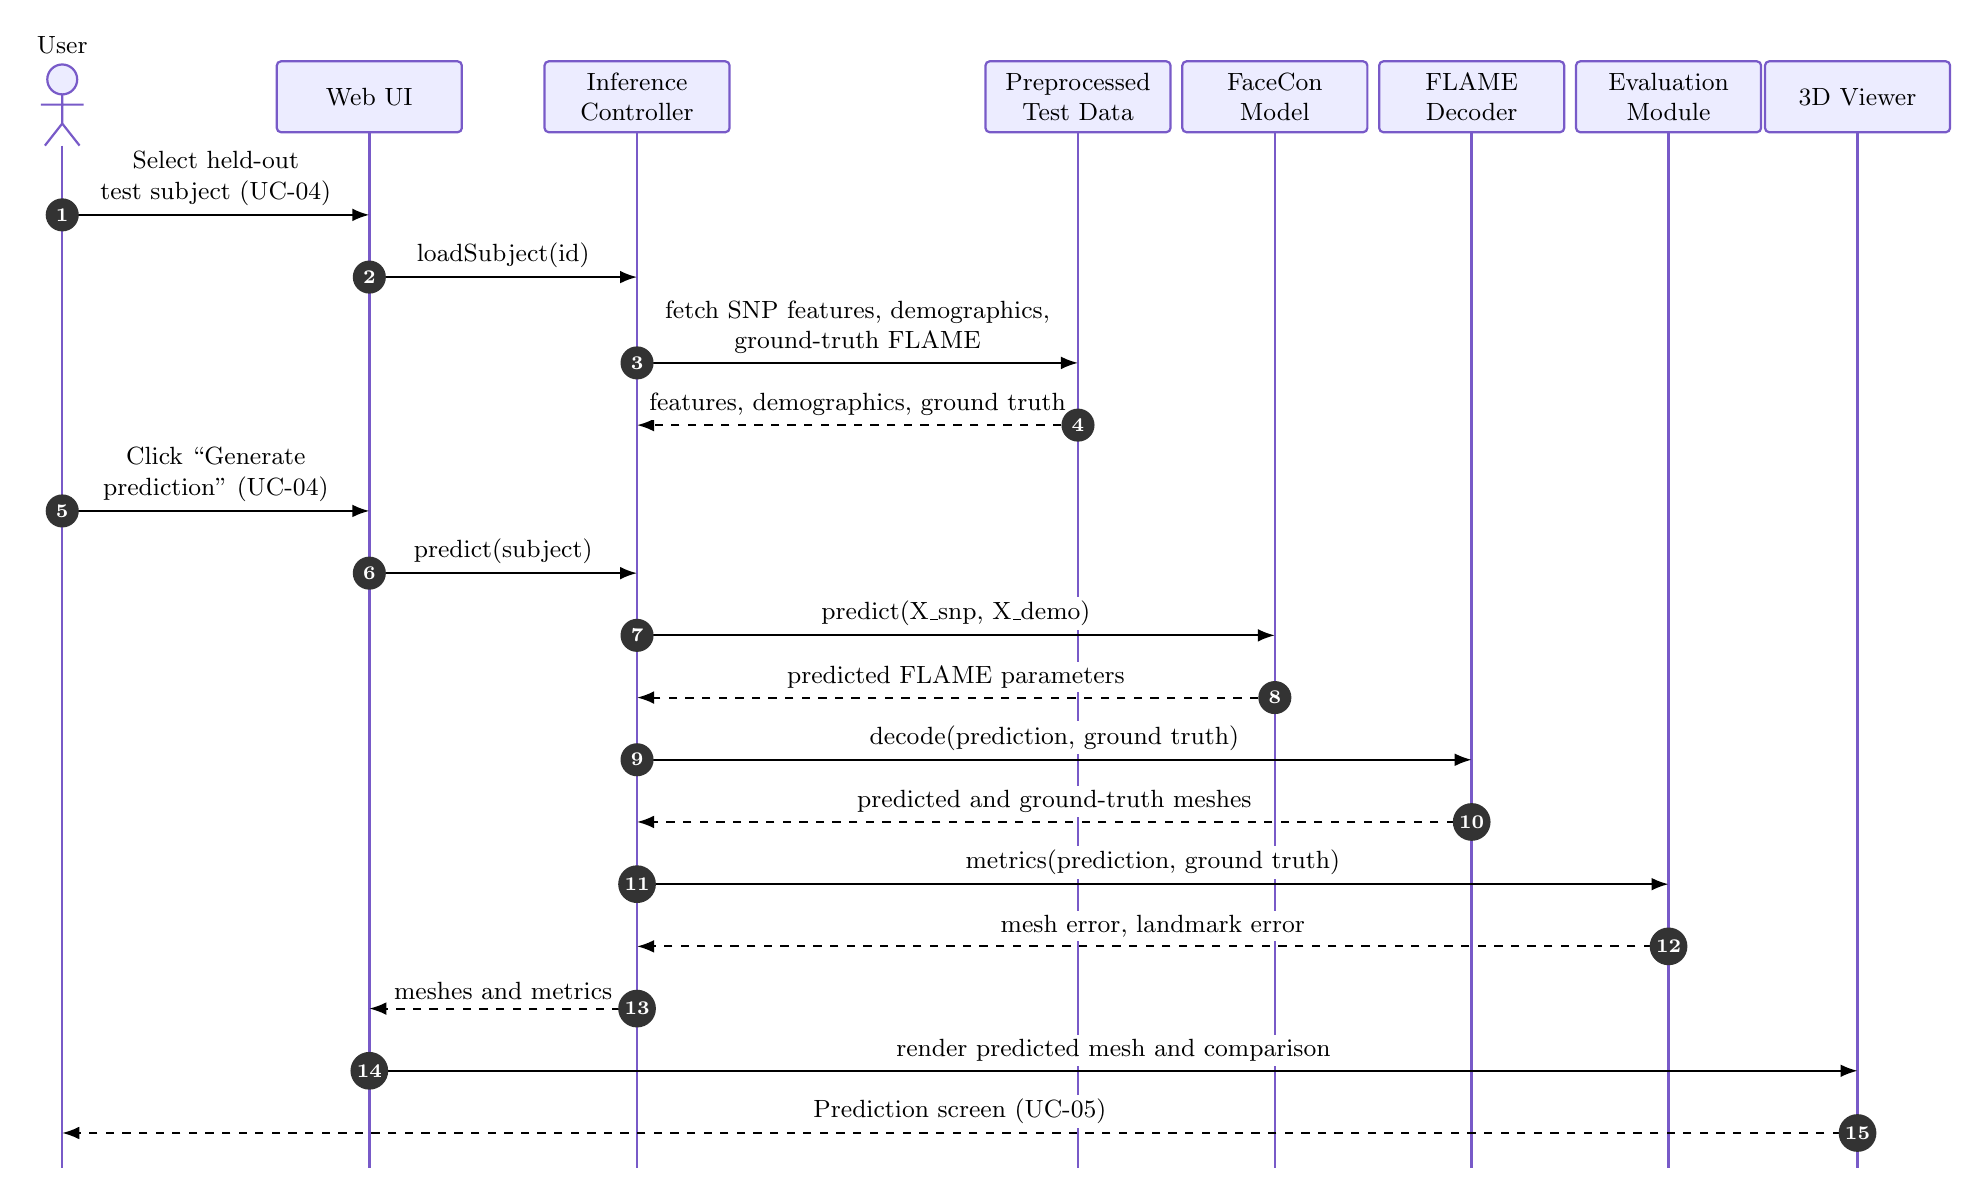
\begin{tikzpicture}[font=\small,>=Latex]
\draw[seqline] (0.5,-0.62)--(0.5,-13.61);
\draw[thick,draw=seqc,fill=seqf] (0.5,0.22) circle (0.19);\draw[thick,draw=seqc] (0.5,0.03)--(0.5,-0.34) (0.22999999999999998,-0.1)--(0.77,-0.1) (0.5,-0.34)--(0.28,-0.62) (0.5,-0.34)--(0.72,-0.62);
\node[anchor=south] at (0.5,0.42) {User};
\draw[seqline] (4.4,-0.45)--(4.4,-13.61);
\node[seqbox] at (4.4,0) {Web UI};
\draw[seqline] (7.8,-0.45)--(7.8,-13.61);
\node[seqbox] at (7.8,0) {Inference\\Controller};
\draw[seqline] (13.4,-0.45)--(13.4,-13.61);
\node[seqbox] at (13.4,0) {Preprocessed\\Test Data};
\draw[seqline] (15.9,-0.45)--(15.9,-13.61);
\node[seqbox] at (15.9,0) {FaceCon\\Model};
\draw[seqline] (18.4,-0.45)--(18.4,-13.61);
\node[seqbox] at (18.4,0) {FLAME\\Decoder};
\draw[seqline] (20.9,-0.45)--(20.9,-13.61);
\node[seqbox] at (20.9,0) {Evaluation\\Module};
\draw[seqline] (23.3,-0.45)--(23.3,-13.61);
\node[seqbox] at (23.3,0) {3D Viewer};
\draw[seqcall] (0.5,-1.50)--(4.4,-1.50);
\draw[seqcall] (4.4,-2.29)--(7.8,-2.29);
\draw[seqcall] (7.8,-3.38)--(13.4,-3.38);
\draw[seqret] (13.4,-4.17)--(7.8,-4.17);
\draw[seqcall] (0.5,-5.26)--(4.4,-5.26);
\draw[seqcall] (4.4,-6.05)--(7.8,-6.05);
\draw[seqcall] (7.8,-6.84)--(15.9,-6.84);
\draw[seqret] (15.9,-7.63)--(7.8,-7.63);
\draw[seqcall] (7.8,-8.42)--(18.4,-8.42);
\draw[seqret] (18.4,-9.21)--(7.8,-9.21);
\draw[seqcall] (7.8,-10.00)--(20.9,-10.00);
\draw[seqret] (20.9,-10.79)--(7.8,-10.79);
\draw[seqret] (7.8,-11.58)--(4.4,-11.58);
\draw[seqcall] (4.4,-12.37)--(23.3,-12.37);
\draw[seqret] (23.3,-13.16)--(0.5,-13.16);
\node[seqlab] at (2.45,-1.44) {Select held-out\\test subject (UC-04)};
\node[seqlab] at (6.10,-2.23) {loadSubject(id)};
\node[seqlab] at (10.60,-3.32) {fetch SNP features, demographics,\\ground-truth FLAME};
\node[seqlab] at (10.60,-4.11) {features, demographics, ground truth};
\node[seqlab] at (2.45,-5.20) {Click ``Generate\\prediction'' (UC-04)};
\node[seqlab] at (6.10,-5.99) {predict(subject)};
\node[seqlab] at (11.85,-6.78) {predict(X\_snp, X\_demo)};
\node[seqlab] at (11.85,-7.57) {predicted FLAME parameters};
\node[seqlab] at (13.10,-8.36) {decode(prediction, ground truth)};
\node[seqlab] at (13.10,-9.15) {predicted and ground-truth meshes};
\node[seqlab] at (14.35,-9.94) {metrics(prediction, ground truth)};
\node[seqlab] at (14.35,-10.73) {mesh error, landmark error};
\node[seqlab] at (6.10,-11.52) {meshes and metrics};
\node[seqlab] at (13.85,-12.31) {render predicted mesh and comparison};
\node[seqlab] at (11.90,-13.10) {Prediction screen (UC-05)};
\node[seqnum] at (0.5,-1.50) {1};
\node[seqnum] at (4.4,-2.29) {2};
\node[seqnum] at (7.8,-3.38) {3};
\node[seqnum] at (13.4,-4.17) {4};
\node[seqnum] at (0.5,-5.26) {5};
\node[seqnum] at (4.4,-6.05) {6};
\node[seqnum] at (7.8,-6.84) {7};
\node[seqnum] at (15.9,-7.63) {8};
\node[seqnum] at (7.8,-8.42) {9};
\node[seqnum] at (18.4,-9.21) {10};
\node[seqnum] at (7.8,-10.00) {11};
\node[seqnum] at (20.9,-10.79) {12};
\node[seqnum] at (7.8,-11.58) {13};
\node[seqnum] at (4.4,-12.37) {14};
\node[seqnum] at (23.3,-13.16) {15};
\end{tikzpicture}

\caption{Sequence diagram for prediction generation (UC-04, UC-03, UC-05).}
\label{fig:seq1}
\end{sidewaysfigure}

Figure~\ref{fig:seq2} shows the evaluation and results interaction (UC-06), in which the inference controller requests the demographic baseline shape, the regional errors, and the summary metrics from the evaluation module and returns them for display.

\begin{sidewaysfigure}
\centering\setstretch{1}
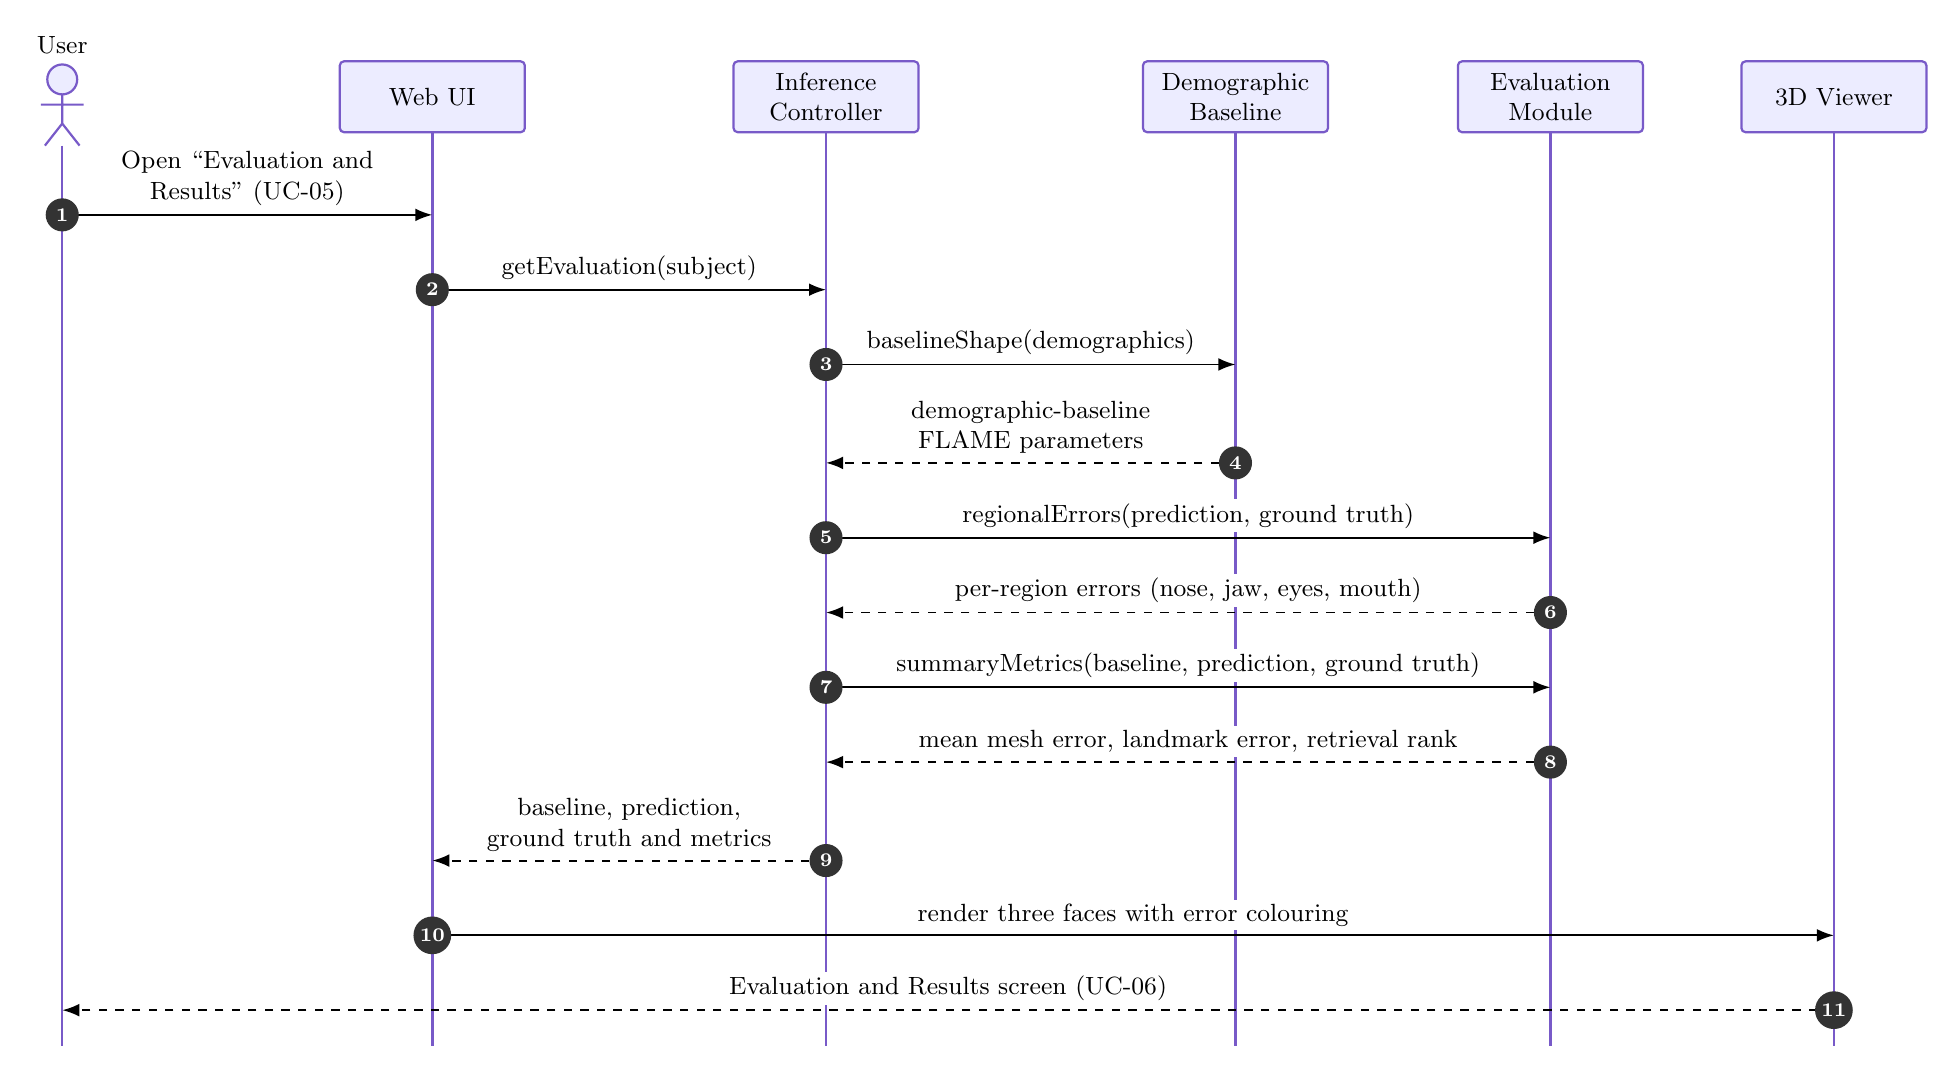
\begin{tikzpicture}[font=\small,>=Latex]
\draw[seqline] (0.5,-0.62)--(0.5,-12.05);
\draw[thick,draw=seqc,fill=seqf] (0.5,0.22) circle (0.19);\draw[thick,draw=seqc] (0.5,0.03)--(0.5,-0.34) (0.22999999999999998,-0.1)--(0.77,-0.1) (0.5,-0.34)--(0.28,-0.62) (0.5,-0.34)--(0.72,-0.62);
\node[anchor=south] at (0.5,0.42) {User};
\draw[seqline] (5.2,-0.45)--(5.2,-12.05);
\node[seqbox] at (5.2,0) {Web UI};
\draw[seqline] (10.2,-0.45)--(10.2,-12.05);
\node[seqbox] at (10.2,0) {Inference\\Controller};
\draw[seqline] (15.4,-0.45)--(15.4,-12.05);
\node[seqbox] at (15.4,0) {Demographic\\Baseline};
\draw[seqline] (19.4,-0.45)--(19.4,-12.05);
\node[seqbox] at (19.4,0) {Evaluation\\Module};
\draw[seqline] (23.0,-0.45)--(23.0,-12.05);
\node[seqbox] at (23.0,0) {3D Viewer};
\draw[seqcall] (0.5,-1.50)--(5.2,-1.50);
\draw[seqcall] (5.2,-2.45)--(10.2,-2.45);
\draw[seqcall] (10.2,-3.40)--(15.4,-3.40);
\draw[seqret] (15.4,-4.65)--(10.2,-4.65);
\draw[seqcall] (10.2,-5.60)--(19.4,-5.60);
\draw[seqret] (19.4,-6.55)--(10.2,-6.55);
\draw[seqcall] (10.2,-7.50)--(19.4,-7.50);
\draw[seqret] (19.4,-8.45)--(10.2,-8.45);
\draw[seqret] (10.2,-9.70)--(5.2,-9.70);
\draw[seqcall] (5.2,-10.65)--(23.0,-10.65);
\draw[seqret] (23.0,-11.60)--(0.5,-11.60);
\node[seqlab] at (2.85,-1.44) {Open ``Evaluation and\\Results'' (UC-05)};
\node[seqlab] at (7.70,-2.39) {getEvaluation(subject)};
\node[seqlab] at (12.80,-3.34) {baselineShape(demographics)};
\node[seqlab] at (12.80,-4.59) {demographic-baseline\\FLAME parameters};
\node[seqlab] at (14.80,-5.54) {regionalErrors(prediction, ground truth)};
\node[seqlab] at (14.80,-6.49) {per-region errors (nose, jaw, eyes, mouth)};
\node[seqlab] at (14.80,-7.44) {summaryMetrics(baseline, prediction, ground truth)};
\node[seqlab] at (14.80,-8.39) {mean mesh error, landmark error, retrieval rank};
\node[seqlab] at (7.70,-9.64) {baseline, prediction,\\ground truth and metrics};
\node[seqlab] at (14.10,-10.59) {render three faces with error colouring};
\node[seqlab] at (11.75,-11.54) {Evaluation and Results screen (UC-06)};
\node[seqnum] at (0.5,-1.50) {1};
\node[seqnum] at (5.2,-2.45) {2};
\node[seqnum] at (10.2,-3.40) {3};
\node[seqnum] at (15.4,-4.65) {4};
\node[seqnum] at (10.2,-5.60) {5};
\node[seqnum] at (19.4,-6.55) {6};
\node[seqnum] at (10.2,-7.50) {7};
\node[seqnum] at (19.4,-8.45) {8};
\node[seqnum] at (10.2,-9.70) {9};
\node[seqnum] at (5.2,-10.65) {10};
\node[seqnum] at (23.0,-11.60) {11};
\end{tikzpicture}

\caption{Sequence diagram for evaluation and results (UC-06).}
\label{fig:seq2}
\end{sidewaysfigure}

Figure~\ref{fig:seq3} shows the simple return interaction, in which the user navigates from the evaluation and results view back to subject selection and the system resets the viewers and reloads the list of held-out subjects.

\begin{figure}[!ht]
\centering\setstretch{1}
% Figure 6.5: return to subject selection (UC-06, UC-04).
% Redrawn as vector graphics in the style of Figures 6.3 and 6.4; the earlier
% raster version used a different typeface and its self-call label crossed the lifeline.
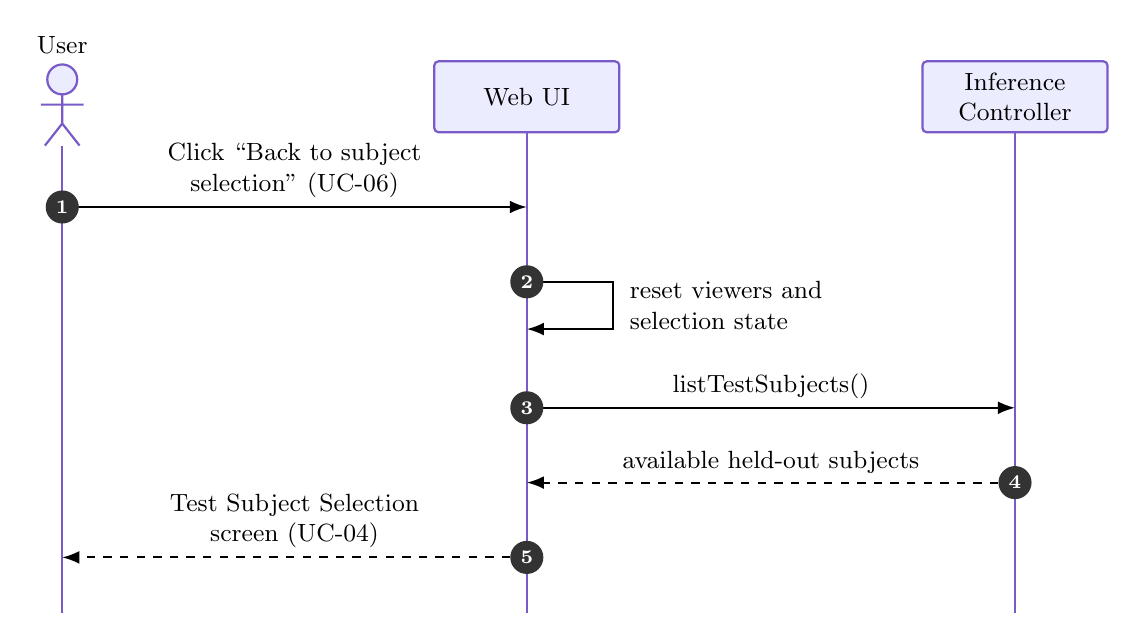
\begin{tikzpicture}[font=\small,>=Latex]
\draw[seqline] (0.5,-0.62)--(0.5,-6.55);
\draw[thick,draw=seqc,fill=seqf] (0.5,0.22) circle (0.19);\draw[thick,draw=seqc] (0.5,0.03)--(0.5,-0.34) (0.23,-0.1)--(0.77,-0.1) (0.5,-0.34)--(0.28,-0.62) (0.5,-0.34)--(0.72,-0.62);
\node[anchor=south] at (0.5,0.42) {User};
\draw[seqline] (6.4,-0.45)--(6.4,-6.55);
\node[seqbox] at (6.4,0) {Web UI};
\draw[seqline] (12.6,-0.45)--(12.6,-6.55);
\node[seqbox] at (12.6,0) {Inference\\Controller};
% messages
\draw[seqcall] (0.5,-1.40)--(6.4,-1.40);
\draw[seqcall] (6.4,-2.35)--(7.5,-2.35)--(7.5,-2.95)--(6.4,-2.95);
\draw[seqcall] (6.4,-3.95)--(12.6,-3.95);
\draw[seqret] (12.6,-4.90)--(6.4,-4.90);
\draw[seqret] (6.4,-5.85)--(0.5,-5.85);
% labels
\node[seqlab] at (3.45,-1.34) {Click ``Back to subject\\selection'' (UC-06)};
\node[anchor=west,inner sep=1.5pt,align=left,font=\small] at (7.65,-2.65) {reset viewers and\\selection state};
\node[seqlab] at (9.50,-3.89) {listTestSubjects()};
\node[seqlab] at (9.50,-4.84) {available held-out subjects};
\node[seqlab] at (3.45,-5.79) {Test Subject Selection\\screen (UC-04)};
% step numbers
\node[seqnum] at (0.5,-1.40) {1};
\node[seqnum] at (6.4,-2.35) {2};
\node[seqnum] at (6.4,-3.95) {3};
\node[seqnum] at (12.6,-4.90) {4};
\node[seqnum] at (6.4,-5.85) {5};
\end{tikzpicture}

\caption{Sequence diagram for returning to subject selection (UC-06, UC-04).}
\label{fig:seq3}
\end{figure}

\section{Policies and Tactics}
This section records design policies and tactics that shape the implementation without altering the high-level architecture. Where the architecture fixes which components exist, these policies fix how they must behave, and most of them exist to protect the validity of the results. They cover the contracts between components, the handling of controlled-access data, reproducibility, the prevention of data leakage, input validation, and the traceability of tests to requirements.

\subsection{Interface Contracts}
\label{sec:interfaces}
The system is held together by six small, explicit interface contracts, which also make synthetic and real data interchangeable.
\begin{itemize}
\item The genotype interface produces $X_{\mathrm{snp}}$ and subject identifiers, and is interchangeable between synthetic and real data loaders.
\item The face interface produces $Y_{\mathrm{face}}$, and optionally a mesh and landmarks, from FLAME fitting.
\item The model interface is \texttt{predict(X\_snp, X\_demo=None) -> Y\_face\_hat}.
\item The decode interface is \texttt{flame\_decode(Y\_face\_hat) -> vertices, faces}.
\item The appearance interface is \texttt{hirisplex\_predict(X\_markers) -> eye, hair, skin colour}, wrapping the external HIrisPlex-S predictor over the extracted marker SNPs, plus a renderer that applies the predicted colours to the decoded mesh.
\item The evaluation interface compares shape predictions and meshes against held-out targets and baselines.
\end{itemize}

\subsection{Data Handling, Privacy, and Access Control}
Raw genotype and scan data are used only under the approved data-use agreement and are never written into released code, figures, or the demonstrator. Raw and processed data are kept in separate locations, and only de-identified, processed artifacts cross into the modelling and demonstration stages. The demonstrator operates on preprocessed test data and never exposes raw genotype information.

\subsection{Reproducibility and Experiment Consistency}
Every run is driven by a configuration file and a fixed random seed, dependencies are pinned, and per-run configurations are captured. All models are evaluated on identical data splits and with the same metric implementations, so that comparisons across the baselines first progression are consistent.

\subsection{Data-Leakage Prevention and Model Selection}
Splits are strictly subject-level and respect relatedness. Any dataset-derived statistics, such as normalization parameters or within-dataset SNP selection, are fitted on the training folds only. Model selection uses the validation split, and the test split is reserved for final reporting.

\subsection{Input Validation and Error Handling}
Each module validates its inputs and fails safely on malformed data, reporting the error and halting rather than producing invalid output. Missing SNPs at inference are imputed or masked according to the documented policy, and subjects that cannot be fitted to FLAME within the error threshold are flagged and excluded with a recorded reason.

\subsection{Coding, Testing, and Traceability}
Coding conventions require modular packages per pipeline stage, typed function signatures, and no hard-coded machine-specific paths. Each module is unit-tested on synthetic inputs, and an end-to-end integration test runs on synthetic data before real data is used. Requirements traceability is maintained by linking each functional requirement to a use case and a planned test.

\section{Conclusion}
This chapter has presented FaceCon's design as a four-layer modular architecture. The interface layer, the processing layer, the model layer, and the data layer each have one responsibility, and they communicate only through the small set of explicit contracts recorded in this chapter. Several architectural strategies were considered, and a layered pipeline with interchangeable models behind a shared interface was selected because it lets the simplest baseline and the most complex network be trained, evaluated, and compared through exactly the same code. The class diagram makes that structure precise, distinguishing the associations, dependencies, and inheritance between the components, and the sequence diagrams show how the main use cases move through them at run time. The policies and tactics turn the requirements of Chapter~\ref{ch:srs} into rules the code must follow, covering privacy and access control, reproducibility, the prevention of data leakage, input validation, and the traceability of tests to requirements. The next chapter describes the prototype that implements this design and the test cases that verify it.

\chapter{Implementation and Test Cases}
\label{ch:impl}
This chapter describes the prototype that implements the methodology of Chapter~\ref{ch:method} and the design of Chapter~\ref{ch:design}, and the test cases used to verify it. Controlled access to the 3DFN data was still pending during this phase, so the prototype was built and exercised on a simulated cohort in which the true relationship between genotype and face is known. This choice has a practical benefit: a pipeline can be tested for correctness only where the right answer is known in advance. The chapter first describes the algorithms and procedures that were implemented, then the design of the test cases, and finally the test metrics.

\section{Implementation}
The prototype implements every stage of the pipeline in Figure~\ref{fig:pipeline} except those that need the real files: genotype QC on real array data and the registration of real scans to FLAME. For those two stages, the interfaces of Section~\ref{sec:interfaces} are in place and are fed by the simulated cohort, so the real loaders can be substituted without changing the modelling or evaluation code.

\subsection{Platform and Tools}
The prototype is written in Python~3. Numerical work uses NumPy and SciPy, the linear baselines and PC analysis use scikit-learn~\cite{ref:sklearn}, and the neural models use PyTorch~\cite{ref:pytorch}. The neural experiments were run on a single NVIDIA RTX A4000 graphics card under Windows with CUDA, and every other stage runs on an ordinary laptop processor. Each experiment is driven by a YAML configuration file and a fixed random seed, as required by NFR-03, and separate named random streams are used for genotypes, faces, splits, and markers so that changing one stage does not disturb another. Automated tests are run with pytest. The demonstrator is a static web page that renders meshes with the three.js library~\cite{ref:threejs}, kept beside the page so that it runs offline. The full source code, the configuration files, the result files behind every number in Chapter~\ref{ch:results}, and the test suite are kept under version control.

\subsection{Simulated Cohort Generator}
\label{sec:impl-cohort}
The generator produces a cohort that follows the public description of the 3DFN GWAS~\cite{ref:shaffer,ref:weinberg}. It contains 3{,}118 subjects, which is the size of that study's analysis sample, with ages between 3 and 49 years and the covariates used in that study: sex, age, age squared, height, and weight. Three synthetic ancestry groups are included on purpose. The real cohort is of European ancestry, so the simulated one is a harder test of confounding than the real data is expected to be.

Genotypes are generated as allele dosages of 0, 1, or 2 for 5{,}000 SNPs. Each SNP is given a base allele frequency between 0.05 and 0.5, and for a quarter of the SNPs the frequency is shifted between ancestry groups, which creates the population structure that a real cohort shows. Each dosage is then drawn from a binomial distribution with two trials. The real genotyping array has close to one million correlated SNPs, so the simulated panel is a deliberately small and simplified subset.

The facial shape target is a 50-dimensional vector $\beta$ per subject. It is composed from three independent sources, each rescaled to a fixed share of the total variance:
\begin{equation}\label{eq:compose}
\beta \;=\; \sqrt{s_g}\,\tilde{G} \;+\; \sqrt{s_d}\,\tilde{D} \;+\; \sqrt{s_e}\,\tilde{E}, \qquad s_g + s_d + s_e = 1 .
\end{equation}
In Equation~\ref{eq:compose}, $\tilde{G}$ is the genetic component, obtained by multiplying the centred dosages of 150 randomly chosen causal SNPs by random weights. $\tilde{D}$ is the demographic component, obtained in the same way from the covariates and the ancestry indicators, with ancestry given a stronger weight so that it acts as a real confounder. $\tilde{E}$ is random noise. Each component is scaled to unit average variance before the shares are applied. The experiments in Chapter~\ref{ch:results} use $s_g = 0.20$, $s_d = 0.35$, and $s_e = 0.45$. The genetic share is a parameter that we control, which is what makes the positive and negative controls of Section~\ref{sec:impl-controls} possible. Subjects are divided at subject level into training, validation, and test sets of 2{,}182, 467, and 469 subjects.

\subsection{Real Genotype Panel}
\label{sec:impl-1kg}
A second cohort replaces the simulated genotypes with real ones while keeping the simulated faces, which removes the main simplifications of the generator without needing the controlled-access data. The genotypes come from the high-coverage release of the 1000 Genomes Project~\cite{ref:kgenomes}, which provides 3{,}202 people sequenced across five continental groups.

The panel is prepared with the PLINK~2 toolkit in two passes. The first pass applies the filters and writes the list of SNPs that survive them. People within the second degree of kinship are removed, which leaves 2{,}573 unrelated subjects, and SNPs are kept only if they lie on the autosomes or the X chromosome, have two alleles, are not insertions or deletions, carry a unique identifier, have a MAF of at least 0.01, and are genotyped in at least 98 per cent of subjects. About 12.7 million SNPs pass. A fixed random seed then selects 100{,}000 of them, and the second pass writes the genotype files for that selection. The second pass does not reapply the filters, so a few identifiers whose duplicates were excluded in the first pass bring those duplicates back, and the panel used in Chapter~\ref{ch:results} holds 100{,}009 columns rather than exactly 100{,}000. The panel is addressed by column and not by identifier, so this is a matter of record rather than of correctness. Two passes are used rather than a single thinning option so that the selection is explicit and reproducible, and a reader can repeat it from the recorded seed. The marker SNPs of the appearance module and the published lead SNPs are extracted separately and without the frequency filter, because the published appearance model needs those exact positions whether they are common or not.

The alleles of the named SNPs must be matched to the published ones, which is the step where a silent error would be most damaging, since a reversed allele inverts the effect it carries. The reader matches an allele exactly where it can, accepts a complementary pair where the SNP is not ambiguous under reversal, and applies a length rule for insertions and deletions. Markers on the X chromosome are handled with the sex of the subject, because males carry one copy rather than two. Every marker is reported as matched by a named rule or as not found, and the build prints the published European frequency of each named SNP beside the frequency measured in the European subjects of the panel, so that a mismatch is visible rather than silent.

The faces for this cohort are composed by the same generator and the same equation, so the only change is the genotype. The effects are made sparse to match the way real effects are believed to act, with 300 causal SNPs that each affect 5 of the 50 shape dimensions rather than all of them. The sex and the continental group of each subject are taken from the real sample table instead of being drawn. The resulting dataset is recorded with a mode of real genotypes and simulated faces, so that no later analysis can present it as anything else.

\subsection{Face Model and Anthropometric Measures}
\label{sec:impl-flame}
FLAME fitting requires the real scans, so the prototype uses a stand-in face model with the same mathematical form. The stand-in is derived from the openly licensed ICT-FaceKit model~\cite{ref:ictfacekit} and consists of a mean mesh of 26{,}719 vertices and 52{,}220 triangles together with 50 identity components. A shape vector is decoded to a mesh as the mean mesh plus a weighted sum of the components, and the result is converted to millimetres. Because every model predicts only the shape vector and decoding happens in one shared component, replacing the stand-in with FLAME is a change to a single module.

From each decoded mesh the prototype computes 20 linear measurements as distances between pairs of 68 facial landmarks, for example the distance between the inner corners of the eyes. These follow the measurement set of the 3DFN association study~\cite{ref:shaffer} as closely as the available landmarks allow. Sixteen of that study's twenty traits are represented, and the remaining measures are close substitutes. Six facial regions (nose, jaw, mouth, eyes, cheeks, and forehead) are also defined on the mesh for the regional analysis planned in Chapter~\ref{ch:method}.

The registration objective of Equation~\ref{eq:fit} is implemented in three stages. A rigid alignment from the landmarks gives an initial pose; closed-form ridge least squares for the shape vector and a rigid realignment are then alternated, since the first alignment matches the mean face rather than the subject's; and finally the shape vector and the pose are optimised together with a symmetric surface term whose point correspondences are recomputed periodically. The weight on the shape prior is set from the generator's own prior and an assumed landmark accuracy rather than tuned. Section~\ref{sec:res-flame} reports what it achieves on synthetic scans, together with the control that distinguishes a fitted face from a mesh that is not one.

Two limits should be read with those numbers. The model being fitted is the stand-in, so the results describe the fitting procedure and not FLAME's own accuracy, and expression, which only the real FLAME model carries, is not fitted. The routine has not been run on real scans, so this stage remains prepared work rather than a validated component of the final system.

\subsection{Injection of Published Association Signals}
\label{sec:impl-inject}
To ground the simulation in published biology, the generator adds real association signals to the measurements. The lead SNP for each of 14 facial traits was taken from the supplementary results of the 3DFN association study~\cite{ref:shaffer}, together with its effect allele, allele frequency, effect size, and standard error. Five of these associations reach genome-wide significance and the other nine are suggestive. One SNP is the lead for two related depth measures and is therefore generated once and shared, and the SNP on the X chromosome is generated so that males carry a single copy.

For a measurement $m$ in standardised form $z_m$ and a lead SNP with standardised dosage $d$, the generator applies
\begin{equation}\label{eq:inject}
z_m' \;=\; \sqrt{1-v}\;z_m \;+\; \operatorname{sign}(b)\,\sqrt{v}\;d ,
\end{equation}
where $b$ is the published effect size and $v$ is the share of variance assigned to the SNP. This form leaves the mean and spread of the measurement unchanged. The share $v$ is derived from the published effect size and standard error as $(b/\mathrm{se})^2/N$ and lies between 0.6 and 1.7 per cent. Because these SNPs were selected for being the strongest in their own discovery sample, this value overstates the true effect and is treated as an upper bound. The injected signals act on the measurements only. They do not enter the shape vector that the models of Chapter~\ref{ch:results} predict.

\subsection{Appearance Module}
\label{sec:impl-appearance}
The appearance module implements the HIrisPlex-S model~\cite{ref:hirisplex,ref:hirisplexs} for the 41 marker SNPs of that system. The model is a set of multinomial logistic regressions on allele dosage. Six markers give the probabilities of blue, intermediate, and brown eye colour. Twenty-two markers give the probabilities of blond, brown, red, and black hair and of a light or dark shade. Thirty-six markers give the probabilities of five skin colour categories. The module returns the probabilities and the most probable category for each trait, and the demonstrator maps the categories to display colours.

One limitation of the current implementation must be stated plainly. The model coefficients in the prototype were not transcribed from the publications. They were recovered by submitting a designed set of genotypes to the public HIrisPlex-S web calculator and solving for the coefficients, which is possible because the model is linear in allele dosage on the log-odds scale. The module therefore reproduces the behaviour of that calculator, but it has not been checked independently against the published parameter tables, and its outputs were never used as training labels for any model. An earlier version of the prototype used a small classifier trained on synthetic colour labels as a placeholder. It was removed, together with its tests, because its labels were generated from the same markers it used as inputs, so its apparent accuracy measured the simulation rather than any ability to predict. In addition, the allele frequencies of the 41 markers in the simulated cohort are synthetic values chosen to give a plausible mix of categories, so the predicted colours in the simulation describe the simulation and not any real population.

\subsection{Feature Construction and Baselines}
\label{sec:impl-features}
All statistics that depend on the data are computed from the training set only, as required by NFR-02. Dosages are standardised with training means and standard deviations. Two SNP representations are then available to the models.
\begin{enumerate}
\item The PC representation projects the standardised dosages onto the leading 256 PCs fitted on the training set.
\item The screened representation keeps the 256 SNPs most associated with shape. The association is measured on the training set only, after the demographic effects have been removed from both the SNPs and the shape vectors by linear regression, and the SNPs are ranked by their summed squared correlation with the shape residuals.
\end{enumerate}
The second representation was added after the controls of Section~\ref{sec:impl-controls} showed that the first one discards most of the planted genetic signal, a finding reported in Chapter~\ref{ch:results}. Four baselines are implemented. They are the mean face, a linear regression on the demographic covariates, a ridge regression on the SNP representation alone, and a ridge regression given exactly what the neural models are given, namely the covariates together with the SNP representation. The last of these is fitted in two stages, with the covariates fitted first without penalty and the SNP features then fitted to the residual, and its penalty is chosen on the validation set. Fitting it in one stage would penalise the covariates alongside the SNPs, which costs the baseline real accuracy when the SNP features are uninformative, as Section~\ref{sec:res-real} describes.

\subsection{Neural Models and Training Procedure}
Four neural models are implemented behind the common model interface, and all of them receive the demographic covariates together with the SNP representation.
\begin{enumerate}
\item The MLP has three hidden layers of 512, 256, and 128 units with dropout, and about 306{,}000 parameters.
\item The Transformer encoder treats each SNP feature as a token, embeds it in 128 dimensions with a learned position, applies three self-attention layers with four heads, averages the tokens, and predicts the shape vector from the pooled representation. It has about 454{,}000 parameters.
\item The contrastive model encodes genotype and face into a shared 128-dimensional space and is trained with a symmetric contrastive loss that pulls matched genotype and face pairs together, combined with a regression head that predicts the shape vector. It has about 147{,}000 parameters.
\item The conditional diffusion model learns to remove noise from a shape vector over 200 steps, conditioned on an embedding of the genotype and demographics, and generates a prediction by running the reverse process from random noise. It has about 225{,}000 parameters.
\end{enumerate}
All four are trained with the AdamW optimiser at a learning rate of $10^{-3}$ and a batch size of 256 for at most 150 epochs. The validation score is computed every ten epochs, and training stops when it has not improved for four consecutive evaluations. The test set is scored once, using the weights from the epoch with the best validation score. This last rule matters in practice: without it, a model that peaks early and then overfits would be judged on its worst state.

\subsection{Controls and Power Analysis}
\label{sec:impl-controls}
A separate script implements the checks that decide whether a result can be trusted. It fits a ladder of linear models of increasing information, from the mean face to covariates, covariates with ancestry PCs, and then SNPs, and reports what the SNPs add beyond covariates and ancestry components. It includes one positive control and two negative controls.
\begin{enumerate}
\item The oracle is a model given the true causal SNPs, which only a simulation can provide. It shows how much signal is available to be found.
\item The permutation control shuffles the genotype rows so that each face is paired with another subject's genotype. Any gain that survives this shuffle would indicate leakage.
\item The null control regenerates the cohort with the genetic share set to zero. A correct pipeline must then report no gain from SNPs.
\end{enumerate}
The script also has a mode in which the causal SNPs are removed from the panel before any model sees it, so that only SNPs correlated with them remain. This mode is meaningful only on real genotypes, where such correlation exists, and it is used for the experiment of Section~\ref{sec:res-ld}. In this mode the oracle is reported for information rather than treated as a check, because whether the neighbours carry the signal is exactly the question being asked.
Each check is repeated over five independently generated cohorts, and a 95 per cent confidence interval is obtained by resampling the test subjects 500 times. The script also repeats the analysis over a grid of cohort sizes and genetic shares to estimate how much signal could be detected at each size. Acceptance thresholds are written into the script, which prints a pass or fail result for each and stops with an error if any fails.

\subsection{Demonstrator}
The demonstrator of Section~\ref{sec:gui} is implemented as a static web page in three views. The first covers the selection and prediction screens designed in Chapter~\ref{ch:srs}. The user picks a held-out subject from the simulated cohort, and the predicted and true faces are shown side by side and rotate together, with the prediction coloured by its error at each vertex. Switching between the mean face, the demographic baseline, the linear reference, and the MLP morphs the prediction to the chosen model, and the error of each model for that subject is listed beside the faces with the HIrisPlex-S colour probabilities. The second view covers the evaluation screen and presents the results of Chapter~\ref{ch:results} for both the simulated and the real genotypes, each with the file it comes from. The third view shows the stages of the pipeline and which data each has been tested on. A separate page presents the same predictions as an animated reveal for the final presentation. Figures~\ref{fig:demo-explore} and~\ref{fig:demo-results} show the first two views. The page opens in a dark theme and offers a light one for bright rooms, which is the one shown here.

\begin{figure}[!ht]
\centering
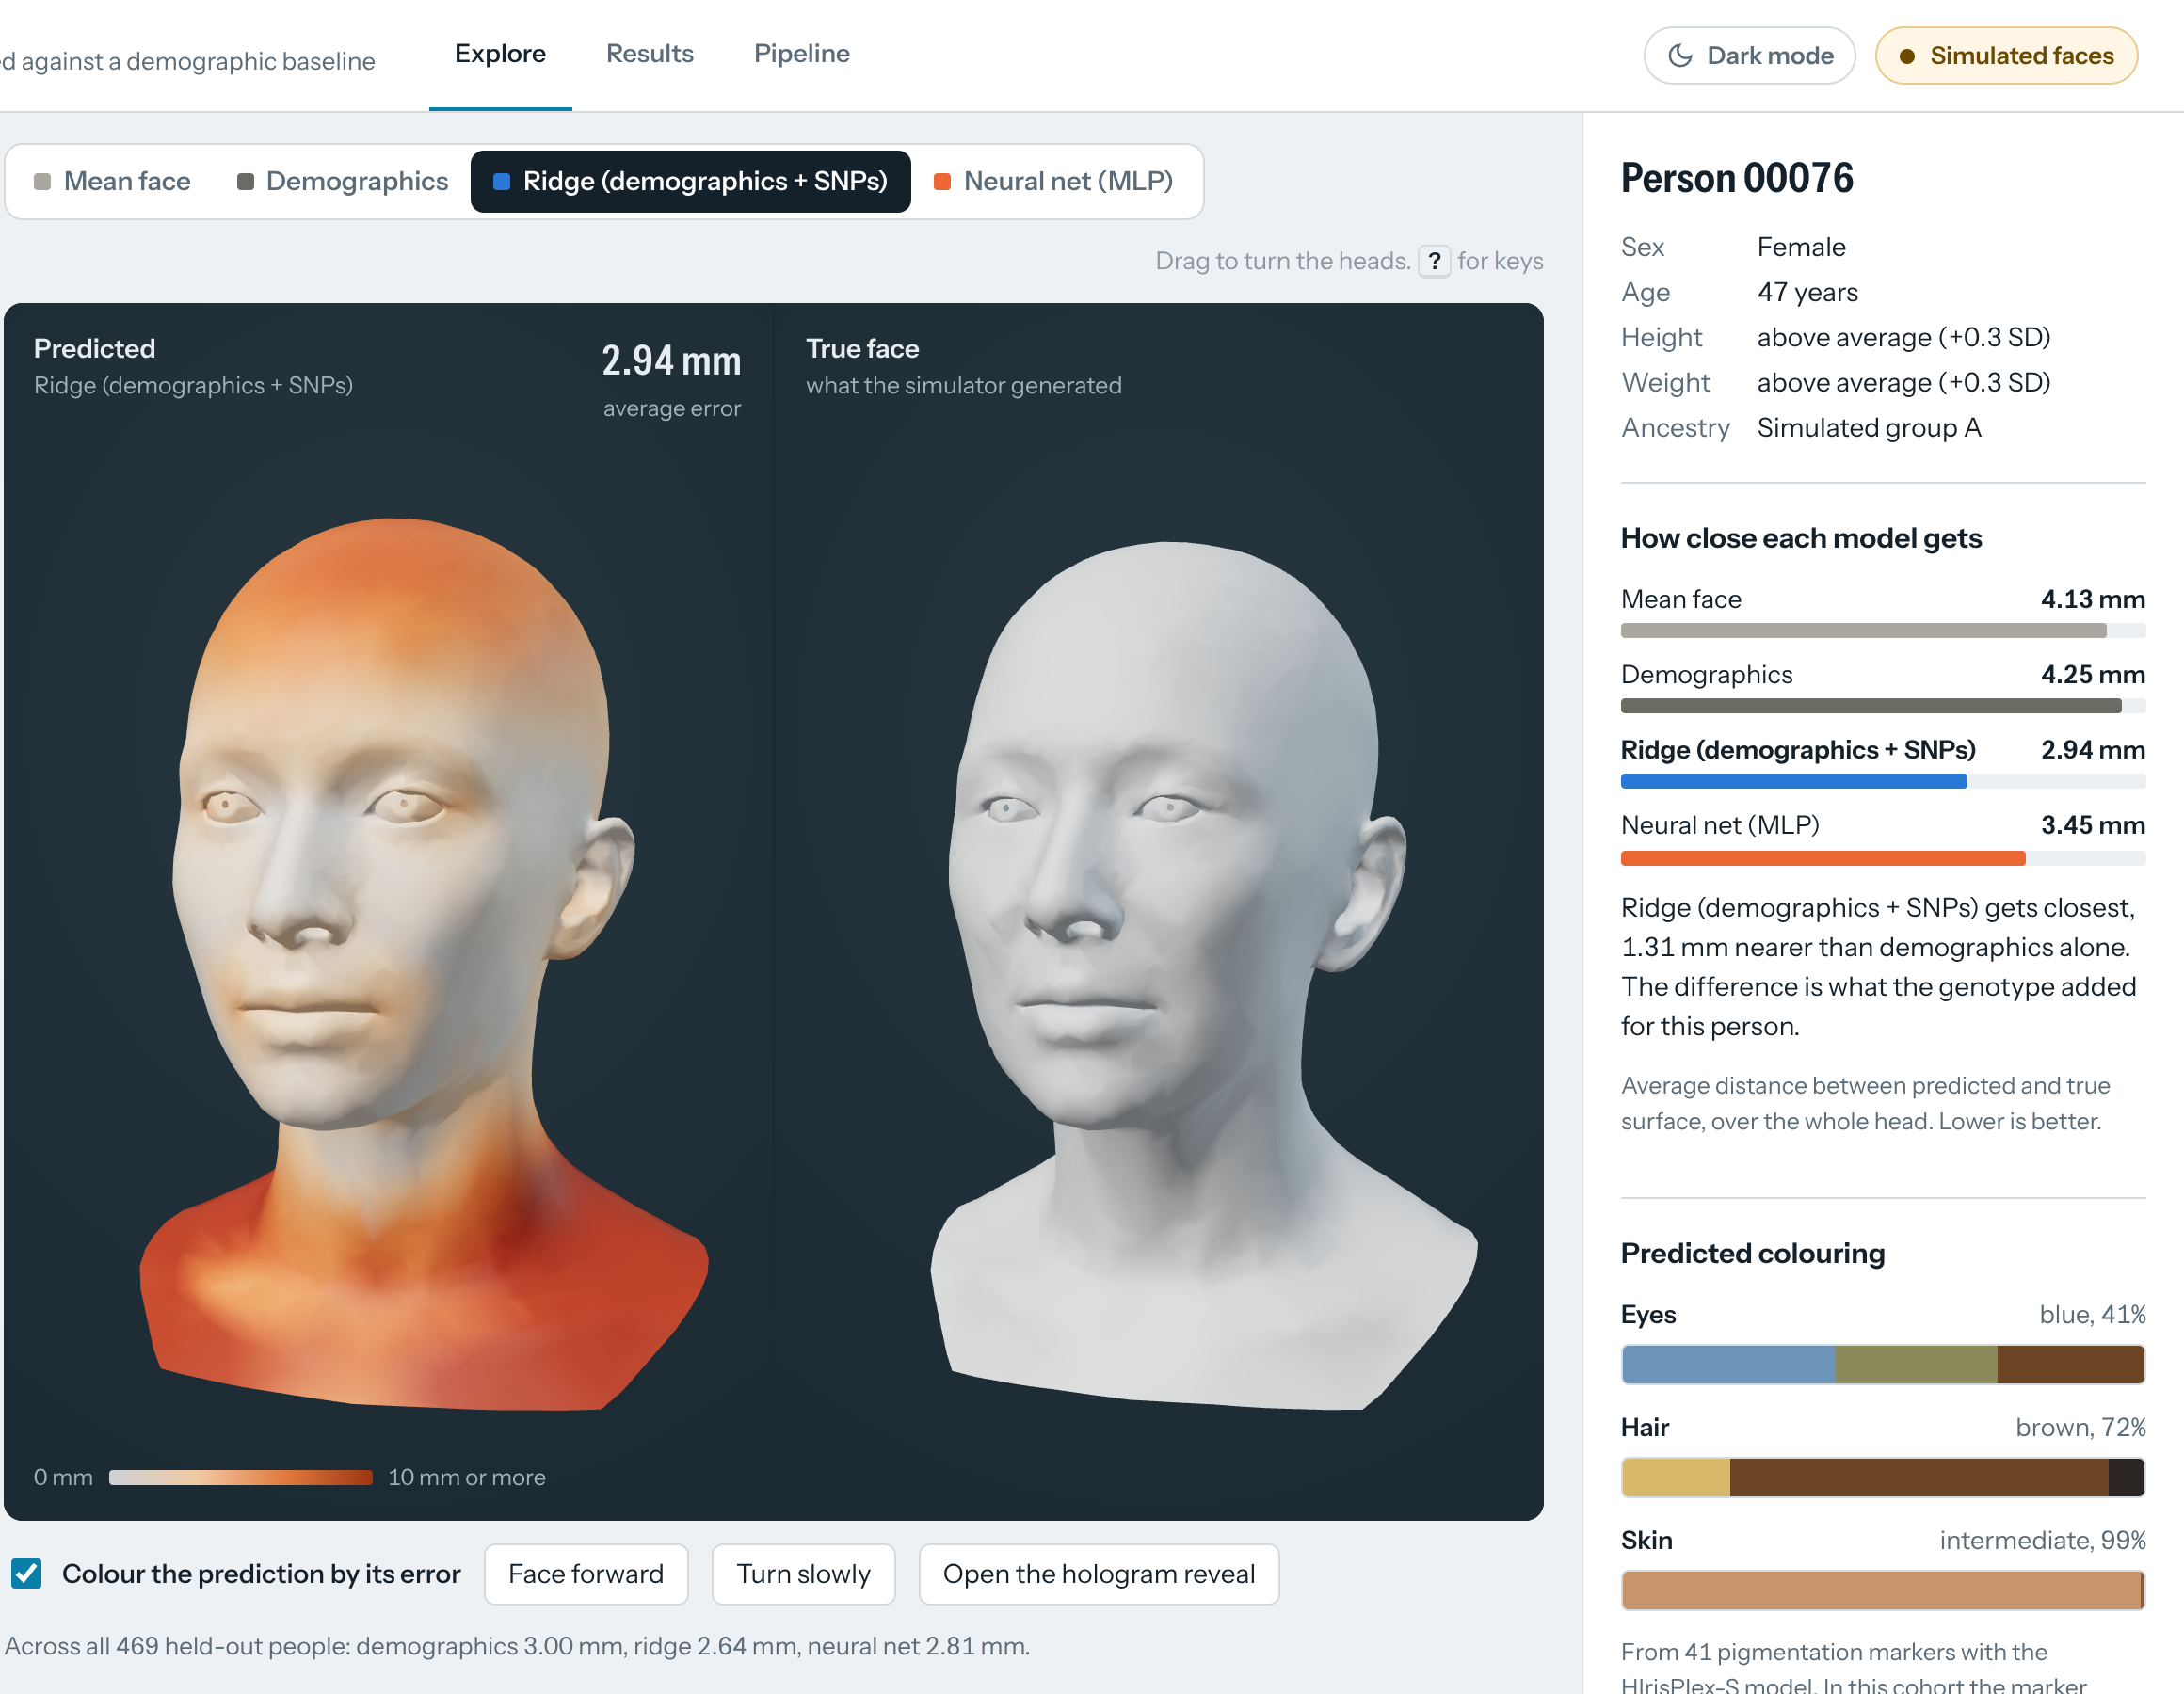
\includegraphics[width=\textwidth]{Figures/demo_explore_crop.png}
\caption{Explore view of the demonstrator, comparing the predicted and true faces for one held-out subject.}
\label{fig:demo-explore}
\end{figure}

\begin{figure}[!ht]
\centering
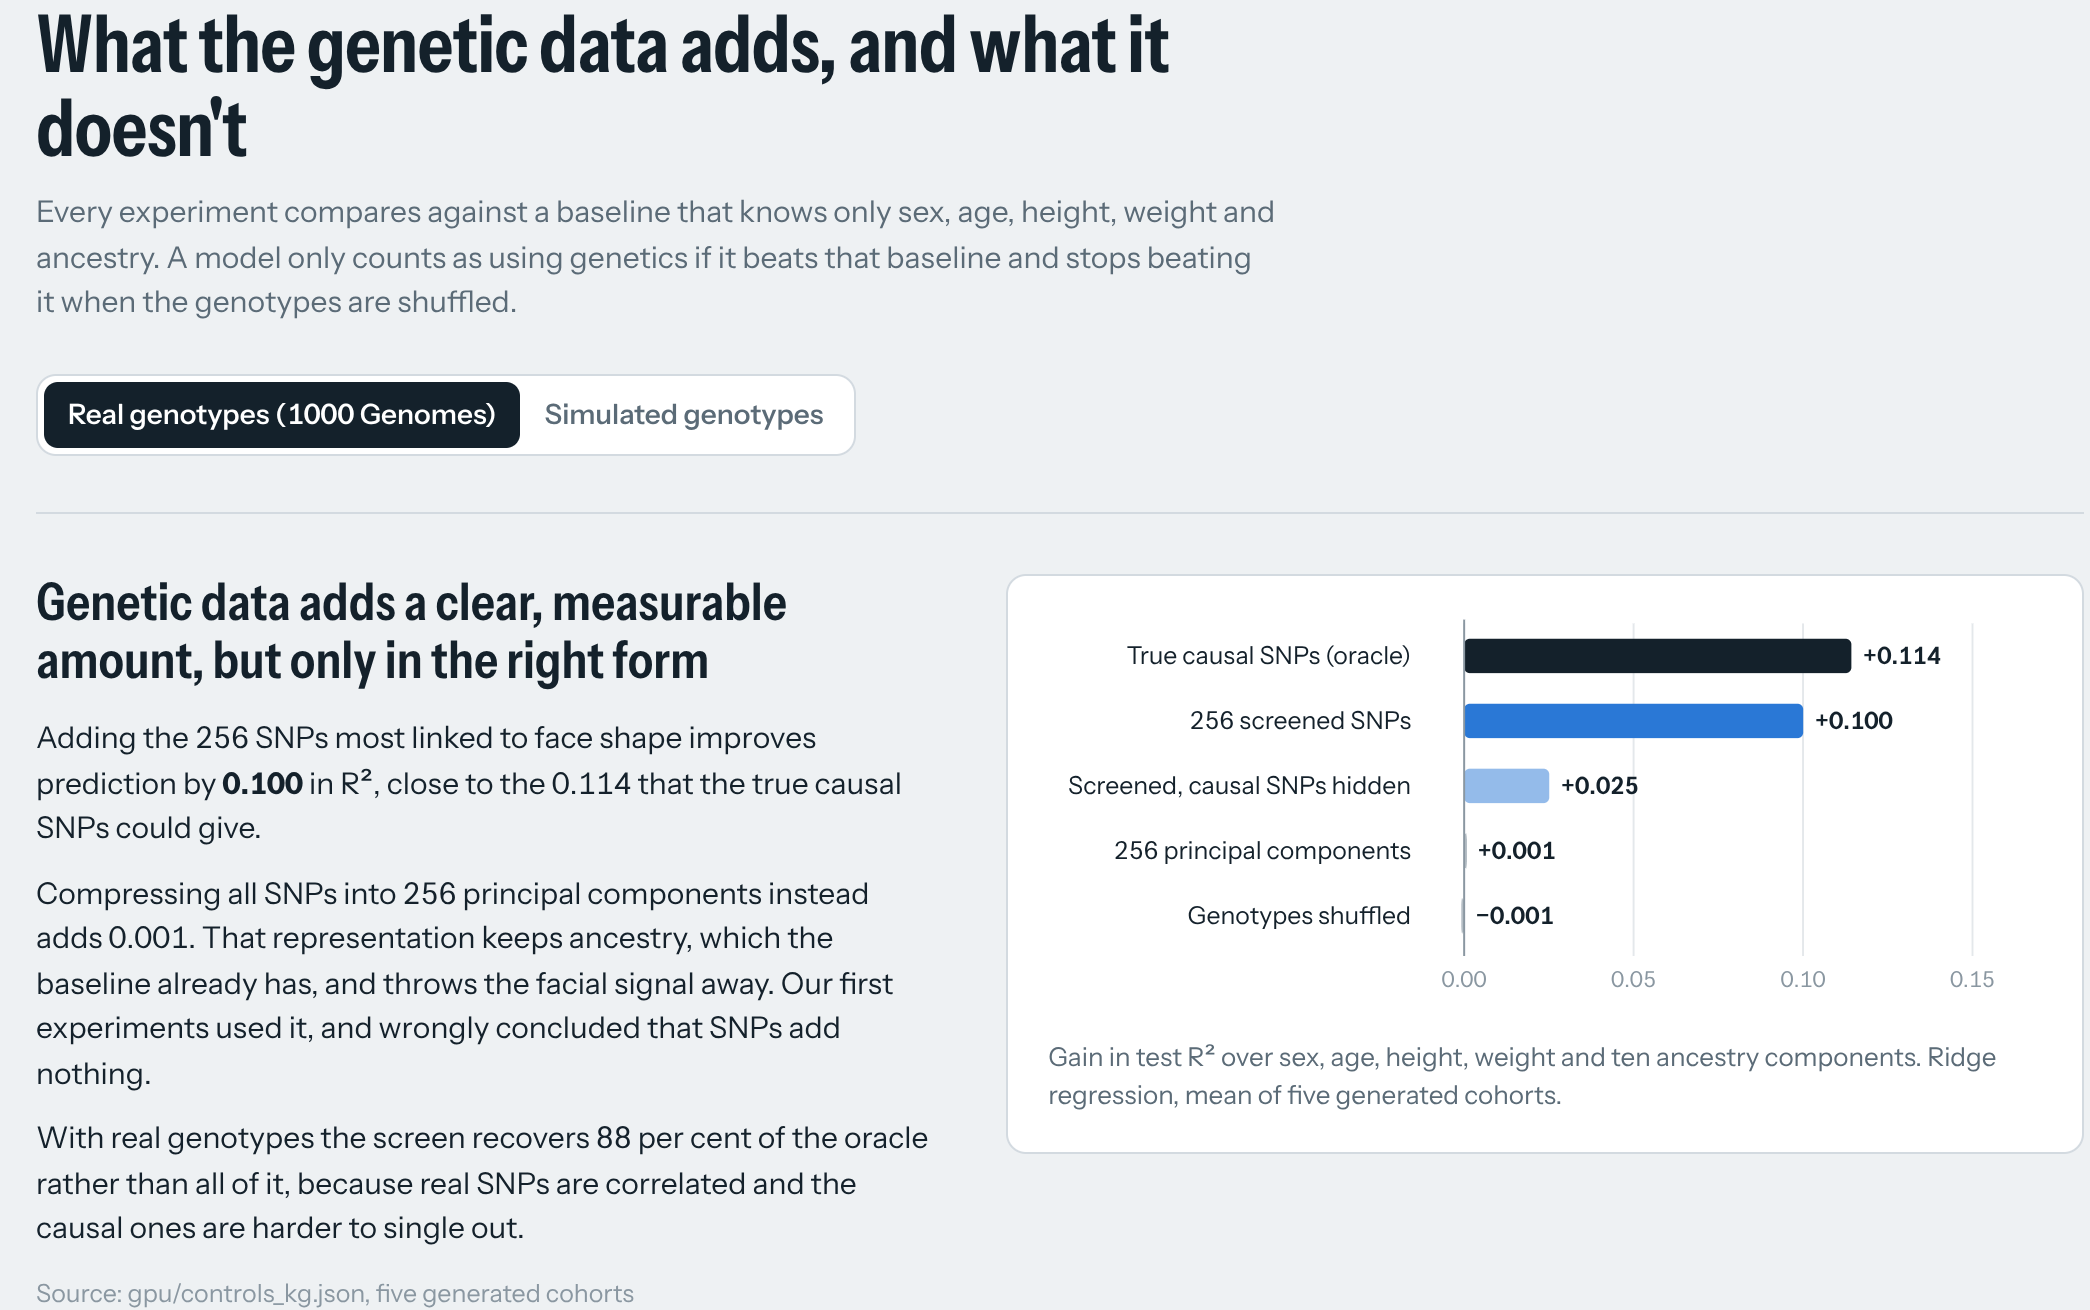
\includegraphics[width=\textwidth]{Figures/demo_results_crop.png}
\caption{Results view of the demonstrator, showing the first finding of the real-genotype experiment.}
\label{fig:demo-results}
\end{figure}

The page reads one precomputed data file and needs no server, so it also works when opened directly from disk. The file is written by an export script from the corrected pipeline of this chapter, using screened SNPs, the two-stage linear reference, and the face decoder with the same scale as the evaluation. Its figures therefore agree with Chapter~\ref{ch:results}, with the demographic baseline at $0.317$ in $R^2$ and $3.00$ millimetres of mesh error on the 469 test subjects. Two departures from the design of Chapter~\ref{ch:srs} should be noted. The face is the stand-in model rather than FLAME, for the reason given in Section~\ref{sec:impl-cohort}, and the baseline is compared through the list of errors and the model switch rather than as a third face on screen.

\section{Test Case Design and Description}
The test cases share the following attributes. Every test runs on simulated data only, so no controlled data is needed to execute the suite. Every test is automated, uses fixed random seeds, and is executed with a single command from the project root. The environment is Python~3 with the packages listed in the project requirements file, and no graphics card is required. The tests fall into three groups: unit tests of individual modules, integration tests that run a stage of the pipeline end to end, and scientific control tests that check a property the results depend on, such as the absence of leakage. Tables~\ref{tab:tc1} to~\ref{tab:tc6} describe six representative test cases in the recommended scheme, and Table~\ref{tab:tcall} lists the complete suite. The last four tests cover the real genotype panel of Section~\ref{sec:impl-1kg}. They run on a small fixture built by the test itself, with the allele cases that caused trouble in practice, so they need no download and no controlled data.


\begin{table}[H]
\caption{Test case TC-01: subject-level splits are disjoint.}
\label{tab:tc1}
\centering\small\setstretch{1.15}
\begin{tabular}{|llll|}
\hline
\multicolumn{4}{|c|}{\textbf{Dataset Builder}} \\ \hline
\multicolumn{4}{|c|}{\textbf{FR-05, NFR-01}} \\ \hline
\multicolumn{1}{|l|}{\textbf{Test Case ID:}} & \multicolumn{1}{l|}{TC-01} & \multicolumn{1}{l|}{\textbf{QA Test Engineer:}} & FaceCon project team \\ \hline
\multicolumn{1}{|l|}{\textbf{Test case Version:}} & \multicolumn{1}{l|}{1.0} & \multicolumn{1}{l|}{\textbf{Reviewed By:}} & FaceCon project team \\ \hline
\multicolumn{1}{|l|}{\textbf{Test Date:}} & \multicolumn{1}{l|}{13 November 2026} & \multicolumn{1}{l|}{\textbf{\begin{tabular}[c]{@{}l@{}}Use Case \\ Reference(s):\end{tabular}}} & UC-01, UC-03 \\ \hline
\multicolumn{1}{|l|}{\textbf{Revision History:}} & \multicolumn{3}{l|}{None} \\ \hline
\multicolumn{1}{|l|}{\textbf{Objective:}} & \multicolumn{3}{p{11.9cm}|}{Verify that no subject appears in more than one of the training, validation, and test sets, and that every subject is assigned.} \\ \hline
\multicolumn{1}{|l|}{\textbf{\begin{tabular}[c]{@{}l@{}}Product/Ver/\\ Module:\end{tabular}}} & \multicolumn{3}{p{11.9cm}|}{FaceCon prototype, simulated cohort generator, split construction.} \\ \hline
\multicolumn{1}{|l|}{\textbf{Environment:}} & \multicolumn{3}{p{11.9cm}|}{Python 3 with the project requirements, processor only, executed with pytest from the project root.} \\ \hline
\multicolumn{1}{|l|}{\textbf{Assumptions:}} & \multicolumn{3}{p{11.9cm}|}{The generator configuration is valid and the random seed is fixed.} \\ \hline
\multicolumn{1}{|l|}{\textbf{Pre-Requisite:}} & \multicolumn{3}{p{11.9cm}|}{None.} \\ \hline
\multicolumn{1}{|l|}{\textbf{Step No.}} & \multicolumn{1}{l|}{\textbf{Execution description}} & \multicolumn{2}{l|}{\textbf{Procedure result}} \\ \hline
\multicolumn{1}{|l|}{1} & \multicolumn{1}{p{5.6cm}|}{Generate a small simulated cohort of 500 subjects.} & \multicolumn{2}{p{6.3cm}|}{Cohort generated with three index sets.} \\ \hline
\multicolumn{1}{|l|}{2} & \multicolumn{1}{p{5.6cm}|}{Concatenate the three index sets and count unique subjects.} & \multicolumn{2}{p{6.3cm}|}{The number of unique subjects equals the cohort size.} \\ \hline
\multicolumn{1}{|l|}{3} & \multicolumn{1}{p{5.6cm}|}{Compare the total number of assigned indices with the cohort size.} & \multicolumn{2}{p{6.3cm}|}{The two numbers are equal, so there is no overlap and no omission.} \\ \hline
\multicolumn{4}{|p{15.2cm}|}{\textbf{Comments:} The controls script repeats this check on every full-size cohort as acceptance check A4.} \\ \hline
\multicolumn{4}{|c|}{\textbf{Passed}} \\ \hline
\end{tabular}
\end{table}

\begin{table}[H]
\caption{Test case TC-02: mesh error is computed at the generator's scale.}
\label{tab:tc2}
\centering\small\setstretch{1.15}
\begin{tabular}{|llll|}
\hline
\multicolumn{4}{|c|}{\textbf{Evaluator}} \\ \hline
\multicolumn{4}{|c|}{\textbf{FR-07, FR-08}} \\ \hline
\multicolumn{1}{|l|}{\textbf{Test Case ID:}} & \multicolumn{1}{l|}{TC-02} & \multicolumn{1}{l|}{\textbf{QA Test Engineer:}} & FaceCon project team \\ \hline
\multicolumn{1}{|l|}{\textbf{Test case Version:}} & \multicolumn{1}{l|}{1.0} & \multicolumn{1}{l|}{\textbf{Reviewed By:}} & FaceCon project team \\ \hline
\multicolumn{1}{|l|}{\textbf{Test Date:}} & \multicolumn{1}{l|}{13 November 2026} & \multicolumn{1}{l|}{\textbf{\begin{tabular}[c]{@{}l@{}}Use Case \\ Reference(s):\end{tabular}}} & UC-03, UC-06 \\ \hline
\multicolumn{1}{|l|}{\textbf{Revision History:}} & \multicolumn{3}{l|}{None} \\ \hline
\multicolumn{1}{|l|}{\textbf{Objective:}} & \multicolumn{3}{p{11.9cm}|}{Verify that the training harness decodes shape vectors with the same face basis and scale as the generator, so that mesh error in millimetres is correct.} \\ \hline
\multicolumn{1}{|l|}{\textbf{\begin{tabular}[c]{@{}l@{}}Product/Ver/\\ Module:\end{tabular}}} & \multicolumn{3}{p{11.9cm}|}{FaceCon prototype, training harness data loader and face model.} \\ \hline
\multicolumn{1}{|l|}{\textbf{Environment:}} & \multicolumn{3}{p{11.9cm}|}{Python 3 with the project requirements, processor only, executed with pytest from the project root.} \\ \hline
\multicolumn{1}{|l|}{\textbf{Assumptions:}} & \multicolumn{3}{p{11.9cm}|}{The stand-in face model file and the generated cohort are present.} \\ \hline
\multicolumn{1}{|l|}{\textbf{Pre-Requisite:}} & \multicolumn{3}{p{11.9cm}|}{Matched simulated cohort generated.} \\ \hline
\multicolumn{1}{|l|}{\textbf{Step No.}} & \multicolumn{1}{l|}{\textbf{Execution description}} & \multicolumn{2}{l|}{\textbf{Procedure result}} \\ \hline
\multicolumn{1}{|l|}{1} & \multicolumn{1}{p{5.6cm}|}{Load the cohort through the training harness.} & \multicolumn{2}{p{6.3cm}|}{The harness holds a face basis.} \\ \hline
\multicolumn{1}{|l|}{2} & \multicolumn{1}{p{5.6cm}|}{Load the face model through the generator's own loader.} & \multicolumn{2}{p{6.3cm}|}{The generator holds a face basis.} \\ \hline
\multicolumn{1}{|l|}{3} & \multicolumn{1}{p{5.6cm}|}{Compare the two bases element by element.} & \multicolumn{2}{p{6.3cm}|}{The bases agree within a relative tolerance of $10^{-4}$.} \\ \hline
\multicolumn{4}{|p{15.2cm}|}{\textbf{Comments:} Written after a review found that the harness omitted the identity scale and under-reported mesh error by a factor of 9.5. The defect is fixed.} \\ \hline
\multicolumn{4}{|c|}{\textbf{Passed}} \\ \hline
\end{tabular}
\end{table}

\begin{table}[H]
\caption{Test case TC-03: published lead SNPs are generated consistently.}
\label{tab:tc3}
\centering\small\setstretch{1.15}
\begin{tabular}{|llll|}
\hline
\multicolumn{4}{|c|}{\textbf{Simulated Cohort Generator}} \\ \hline
\multicolumn{4}{|c|}{\textbf{FR-01}} \\ \hline
\multicolumn{1}{|l|}{\textbf{Test Case ID:}} & \multicolumn{1}{l|}{TC-03} & \multicolumn{1}{l|}{\textbf{QA Test Engineer:}} & FaceCon project team \\ \hline
\multicolumn{1}{|l|}{\textbf{Test case Version:}} & \multicolumn{1}{l|}{1.0} & \multicolumn{1}{l|}{\textbf{Reviewed By:}} & FaceCon project team \\ \hline
\multicolumn{1}{|l|}{\textbf{Test Date:}} & \multicolumn{1}{l|}{13 November 2026} & \multicolumn{1}{l|}{\textbf{\begin{tabular}[c]{@{}l@{}}Use Case \\ Reference(s):\end{tabular}}} & UC-01 \\ \hline
\multicolumn{1}{|l|}{\textbf{Revision History:}} & \multicolumn{3}{l|}{None} \\ \hline
\multicolumn{1}{|l|}{\textbf{Objective:}} & \multicolumn{3}{p{11.9cm}|}{Verify that each published lead SNP is generated once even when it is the lead for several traits, and that the X-chromosome SNP respects sex.} \\ \hline
\multicolumn{1}{|l|}{\textbf{\begin{tabular}[c]{@{}l@{}}Product/Ver/\\ Module:\end{tabular}}} & \multicolumn{3}{p{11.9cm}|}{FaceCon prototype, injection of published association signals.} \\ \hline
\multicolumn{1}{|l|}{\textbf{Environment:}} & \multicolumn{3}{p{11.9cm}|}{Python 3 with the project requirements, processor only, executed with pytest from the project root.} \\ \hline
\multicolumn{1}{|l|}{\textbf{Assumptions:}} & \multicolumn{3}{p{11.9cm}|}{The effect table lists one lead SNP per trait.} \\ \hline
\multicolumn{1}{|l|}{\textbf{Pre-Requisite:}} & \multicolumn{3}{p{11.9cm}|}{Matched simulated cohort generated.} \\ \hline
\multicolumn{1}{|l|}{\textbf{Step No.}} & \multicolumn{1}{l|}{\textbf{Execution description}} & \multicolumn{2}{l|}{\textbf{Procedure result}} \\ \hline
\multicolumn{1}{|l|}{1} & \multicolumn{1}{p{5.6cm}|}{Read the marker identifiers and the marker matrix.} & \multicolumn{2}{p{6.3cm}|}{The number of columns equals the number of unique identifiers.} \\ \hline
\multicolumn{1}{|l|}{2} & \multicolumn{1}{p{5.6cm}|}{Select male subjects at the X-chromosome SNP.} & \multicolumn{2}{p{6.3cm}|}{No male subject has a dosage of one.} \\ \hline
\multicolumn{1}{|l|}{3} & \multicolumn{1}{p{5.6cm}|}{Select female subjects at the same SNP.} & \multicolumn{2}{p{6.3cm}|}{Dosages of one are present, as expected for two copies.} \\ \hline
\multicolumn{4}{|p{15.2cm}|}{\textbf{Comments:} Written after a review found a lead SNP generated as two unrelated columns and an X-chromosome SNP generated without regard to sex. Both defects are fixed.} \\ \hline
\multicolumn{4}{|c|}{\textbf{Passed}} \\ \hline
\end{tabular}
\end{table}

\begin{table}[H]
\caption{Test case TC-04: injected associations are recovered and no others.}
\label{tab:tc4}
\centering\small\setstretch{1.15}
\begin{tabular}{|llll|}
\hline
\multicolumn{4}{|c|}{\textbf{Simulated Cohort Generator}} \\ \hline
\multicolumn{4}{|c|}{\textbf{NFR-06}} \\ \hline
\multicolumn{1}{|l|}{\textbf{Test Case ID:}} & \multicolumn{1}{l|}{TC-04} & \multicolumn{1}{l|}{\textbf{QA Test Engineer:}} & FaceCon project team \\ \hline
\multicolumn{1}{|l|}{\textbf{Test case Version:}} & \multicolumn{1}{l|}{1.0} & \multicolumn{1}{l|}{\textbf{Reviewed By:}} & FaceCon project team \\ \hline
\multicolumn{1}{|l|}{\textbf{Test Date:}} & \multicolumn{1}{l|}{13 November 2026} & \multicolumn{1}{l|}{\textbf{\begin{tabular}[c]{@{}l@{}}Use Case \\ Reference(s):\end{tabular}}} & UC-03 \\ \hline
\multicolumn{1}{|l|}{\textbf{Revision History:}} & \multicolumn{3}{l|}{None} \\ \hline
\multicolumn{1}{|l|}{\textbf{Objective:}} & \multicolumn{3}{p{11.9cm}|}{Verify that an association scan adjusted for covariates detects the injected SNP and measurement pairs, and does not report pairs that were not injected.} \\ \hline
\multicolumn{1}{|l|}{\textbf{\begin{tabular}[c]{@{}l@{}}Product/Ver/\\ Module:\end{tabular}}} & \multicolumn{3}{p{11.9cm}|}{FaceCon prototype, association recovery check stored with the cohort.} \\ \hline
\multicolumn{1}{|l|}{\textbf{Environment:}} & \multicolumn{3}{p{11.9cm}|}{Python 3 with the project requirements, processor only, executed with pytest from the project root.} \\ \hline
\multicolumn{1}{|l|}{\textbf{Assumptions:}} & \multicolumn{3}{p{11.9cm}|}{Both the measurements and the dosages are adjusted for sex, age, age squared, height, weight, and ancestry before testing.} \\ \hline
\multicolumn{1}{|l|}{\textbf{Pre-Requisite:}} & \multicolumn{3}{p{11.9cm}|}{Matched simulated cohort generated.} \\ \hline
\multicolumn{1}{|l|}{\textbf{Step No.}} & \multicolumn{1}{l|}{\textbf{Execution description}} & \multicolumn{2}{l|}{\textbf{Procedure result}} \\ \hline
\multicolumn{1}{|l|}{1} & \multicolumn{1}{p{5.6cm}|}{Test all 260 pairs of SNP and measurement.} & \multicolumn{2}{p{6.3cm}|}{A p-value is obtained for every pair.} \\ \hline
\multicolumn{1}{|l|}{2} & \multicolumn{1}{p{5.6cm}|}{Apply a Bonferroni threshold to the 14 injected pairs (positive control).} & \multicolumn{2}{p{6.3cm}|}{All 14 are detected with the published direction of effect.} \\ \hline
\multicolumn{1}{|l|}{3} & \multicolumn{1}{p{5.6cm}|}{Apply the same threshold to the 246 pairs that were not injected (negative control).} & \multicolumn{2}{p{6.3cm}|}{None is detected, and 2.8 per cent fall below 0.05, which is consistent with chance.} \\ \hline
\multicolumn{4}{|p{15.2cm}|}{\textbf{Comments:} The acceptance rule requires at least 80 per cent of injected pairs to be detected and no false detection.} \\ \hline
\multicolumn{4}{|c|}{\textbf{Passed}} \\ \hline
\end{tabular}
\end{table}

\begin{table}[H]
\caption{Test case TC-05: SNP signal is found when planted and absent when broken.}
\label{tab:tc5}
\centering\small\setstretch{1.15}
\begin{tabular}{|llll|}
\hline
\multicolumn{4}{|c|}{\textbf{Controls and Baseline Ladder}} \\ \hline
\multicolumn{4}{|c|}{\textbf{FR-09, NFR-06}} \\ \hline
\multicolumn{1}{|l|}{\textbf{Test Case ID:}} & \multicolumn{1}{l|}{TC-05} & \multicolumn{1}{l|}{\textbf{QA Test Engineer:}} & FaceCon project team \\ \hline
\multicolumn{1}{|l|}{\textbf{Test case Version:}} & \multicolumn{1}{l|}{1.0} & \multicolumn{1}{l|}{\textbf{Reviewed By:}} & FaceCon project team \\ \hline
\multicolumn{1}{|l|}{\textbf{Test Date:}} & \multicolumn{1}{l|}{13 November 2026} & \multicolumn{1}{l|}{\textbf{\begin{tabular}[c]{@{}l@{}}Use Case \\ Reference(s):\end{tabular}}} & UC-03 \\ \hline
\multicolumn{1}{|l|}{\textbf{Revision History:}} & \multicolumn{3}{l|}{None} \\ \hline
\multicolumn{1}{|l|}{\textbf{Objective:}} & \multicolumn{3}{p{11.9cm}|}{Verify that screened SNPs improve prediction beyond covariates and ancestry components when a genetic share is planted, and that the improvement disappears when the genotype rows are shuffled.} \\ \hline
\multicolumn{1}{|l|}{\textbf{\begin{tabular}[c]{@{}l@{}}Product/Ver/\\ Module:\end{tabular}}} & \multicolumn{3}{p{11.9cm}|}{FaceCon prototype, controls script.} \\ \hline
\multicolumn{1}{|l|}{\textbf{Environment:}} & \multicolumn{3}{p{11.9cm}|}{Python 3 with the project requirements, processor only, executed with pytest from the project root.} \\ \hline
\multicolumn{1}{|l|}{\textbf{Assumptions:}} & \multicolumn{3}{p{11.9cm}|}{A genetic share of 0.20 is planted. Screening and all scaling use the training set only.} \\ \hline
\multicolumn{1}{|l|}{\textbf{Pre-Requisite:}} & \multicolumn{3}{p{11.9cm}|}{None. The test generates its own cohort of 1{,}000 subjects.} \\ \hline
\multicolumn{1}{|l|}{\textbf{Step No.}} & \multicolumn{1}{l|}{\textbf{Execution description}} & \multicolumn{2}{l|}{\textbf{Procedure result}} \\ \hline
\multicolumn{1}{|l|}{1} & \multicolumn{1}{p{5.6cm}|}{Fit the ladder on the generated cohort (positive control).} & \multicolumn{2}{p{6.3cm}|}{The gain from screened SNPs exceeds 0.03 in $R^2$.} \\ \hline
\multicolumn{1}{|l|}{2} & \multicolumn{1}{p{5.6cm}|}{Shuffle the genotype rows and fit again (negative control).} & \multicolumn{2}{p{6.3cm}|}{The gain is below 0.01 in $R^2$.} \\ \hline
\multicolumn{4}{|p{15.2cm}|}{\textbf{Comments:} The full-size version of this test, with five cohorts and confidence intervals, is reported in Chapter~\ref{ch:results}.} \\ \hline
\multicolumn{4}{|c|}{\textbf{Passed}} \\ \hline
\end{tabular}
\end{table}

\begin{table}[H]
\caption{Test case TC-06: appearance predictions are not degenerate.}
\label{tab:tc6}
\centering\small\setstretch{1.15}
\begin{tabular}{|llll|}
\hline
\multicolumn{4}{|c|}{\textbf{Appearance Module}} \\ \hline
\multicolumn{4}{|c|}{\textbf{FR-11, FR-12}} \\ \hline
\multicolumn{1}{|l|}{\textbf{Test Case ID:}} & \multicolumn{1}{l|}{TC-06} & \multicolumn{1}{l|}{\textbf{QA Test Engineer:}} & FaceCon project team \\ \hline
\multicolumn{1}{|l|}{\textbf{Test case Version:}} & \multicolumn{1}{l|}{1.0} & \multicolumn{1}{l|}{\textbf{Reviewed By:}} & FaceCon project team \\ \hline
\multicolumn{1}{|l|}{\textbf{Test Date:}} & \multicolumn{1}{l|}{13 November 2026} & \multicolumn{1}{l|}{\textbf{\begin{tabular}[c]{@{}l@{}}Use Case \\ Reference(s):\end{tabular}}} & UC-03, UC-05 \\ \hline
\multicolumn{1}{|l|}{\textbf{Revision History:}} & \multicolumn{3}{l|}{None} \\ \hline
\multicolumn{1}{|l|}{\textbf{Objective:}} & \multicolumn{3}{p{11.9cm}|}{Verify that the appearance module does not assign nearly every subject to one category for eye, hair, or skin colour.} \\ \hline
\multicolumn{1}{|l|}{\textbf{\begin{tabular}[c]{@{}l@{}}Product/Ver/\\ Module:\end{tabular}}} & \multicolumn{3}{p{11.9cm}|}{FaceCon prototype, appearance module and marker generation.} \\ \hline
\multicolumn{1}{|l|}{\textbf{Environment:}} & \multicolumn{3}{p{11.9cm}|}{Python 3 with the project requirements, processor only, executed with pytest from the project root.} \\ \hline
\multicolumn{1}{|l|}{\textbf{Assumptions:}} & \multicolumn{3}{p{11.9cm}|}{The marker allele frequencies stored with the project are used.} \\ \hline
\multicolumn{1}{|l|}{\textbf{Pre-Requisite:}} & \multicolumn{3}{p{11.9cm}|}{Matched simulated cohort generated.} \\ \hline
\multicolumn{1}{|l|}{\textbf{Step No.}} & \multicolumn{1}{l|}{\textbf{Execution description}} & \multicolumn{2}{l|}{\textbf{Procedure result}} \\ \hline
\multicolumn{1}{|l|}{1} & \multicolumn{1}{p{5.6cm}|}{Predict eye, hair, and skin colour for every subject.} & \multicolumn{2}{p{6.3cm}|}{A category is returned for each trait and subject.} \\ \hline
\multicolumn{1}{|l|}{2} & \multicolumn{1}{p{5.6cm}|}{Compute the share of the most frequent category for each trait.} & \multicolumn{2}{p{6.3cm}|}{The share is below 90 per cent for all three traits.} \\ \hline
\multicolumn{4}{|p{15.2cm}|}{\textbf{Comments:} Written after regenerating the cohort silently reset the marker frequencies and every subject was predicted to have red hair. This test checks plausibility of the simulated inputs and is not a measure of accuracy.} \\ \hline
\multicolumn{4}{|c|}{\textbf{Passed}} \\ \hline
\end{tabular}
\end{table}

\begin{table}[H]
\centering
\caption{The complete automated test suite. All 44 test cases passed in the final run.}
\label{tab:tcall}
\small\setstretch{1.1}
\begin{tabular}{|p{0.9cm}|p{9.3cm}|p{1.9cm}|p{1.9cm}|}
\hline
\textbf{No.} & \textbf{What the test verifies} & \textbf{Type} & \textbf{Detailed in} \\ \hline
T01 & Published lead SNPs generated once, with sex-aware X chromosome & Control & TC-03 \\ \hline
T02 & Injected associations recovered, with no false detections & Control & TC-04 \\ \hline
T03 & Feature matrices have the expected shapes & Unit & --- \\ \hline
T04 & Configuration loads and variance shares sum to one & Unit & --- \\ \hline
T05 & Named random streams are reproducible and independent & Unit & --- \\ \hline
T06 & Dosages take only the values 0, 1, and 2, and shapes are consistent & Unit & --- \\ \hline
T07 & Splits are disjoint and cover every subject & Control & TC-01 \\ \hline
T08 & Realised variance shares match the configuration & Integration & --- \\ \hline
T09 & Saving and reloading a cohort returns identical data & Integration & --- \\ \hline
T10 & Generation is bit-for-bit unchanged when no architecture block is set & Control & --- \\ \hline
T11 & The committed real-match cohort regenerates exactly from its seed & Control & --- \\ \hline
T12 & Quality-control statistics are fitted on the training set only & Control & --- \\ \hline
T13 & Baselines rank sensibly, with the mean face near zero & Integration & --- \\ \hline
T14 & Full evaluation returns every metric for every model & Integration & --- \\ \hline
T15 & Planted signal is recovered above a shuffled-label control & Control & --- \\ \hline
T16 & Mesh error uses the generator's face basis and scale & Control & TC-02 \\ \hline
T17 & Appearance predictions are not degenerate & Control & TC-06 \\ \hline
T18 & SNP signal found when planted and absent when shuffled & Control & TC-05 \\ \hline
T19 & Genotype files are written and read back identically, including missing calls & Unit & --- \\ \hline
T20 & Published alleles are matched to the panel by the documented rules, and ambiguous ones are refused & Unit & --- \\ \hline
T21 & Real genotypes run end to end, from panel to features to controls & Integration & --- \\ \hline
T22 & Sparse genetic effects touch only the chosen shape dimensions & Control & --- \\ \hline
T23--T25 & Dominance and interaction shares are realised at the configured sizes, once for each of the three architectures & Integration & --- \\ \hline
T26 & Heterozygote coding is correct when dosages have been mean-imputed & Unit & --- \\ \hline
T27 & Non-additive weights stay sparse, one row at a time & Unit & --- \\ \hline
T28 & The architecture block is validated, and impossible fractions are refused & Unit & --- \\ \hline
T29 & The processor-only harness refuses non-additive configurations rather than running them wrongly & Control & --- \\ \hline
T30--T32 & Correctly coded non-additive signal scores above a shuffled control, once for each of the three architectures & Control & --- \\ \hline
T33 & A zero genetic share reports nothing through the non-additive rows & Control & --- \\ \hline
T34 & The column-count cost of the non-additive oracle on an additive target is a cost, and keeps its measured size & Control & --- \\ \hline
T35 & The two-degree-of-freedom screen beats the additive screen on a dominance cohort & Control & --- \\ \hline
T36 & A stored split is reproduced exactly from its split seed & Control & --- \\ \hline
T37 & A different split seed redraws the split and still partitions the cohort & Control & --- \\ \hline
T38 & The generator refuses to overwrite the tracked cohort without an explicit override & Control & --- \\ \hline
T39 & The rotation parameterisation returns genuine rotations & Unit & --- \\ \hline
T40 & Scan fitting recovers the shape vector of a noise-free synthetic scan & Integration & --- \\ \hline
T41 & The iterative stage improves on the closed-form landmark warm start & Integration & --- \\ \hline
T42 & A mesh of noise gives a far larger fit residual than a real face & Control & --- \\ \hline
T43 & Scan fitting is reproducible from its seed & Unit & --- \\ \hline
T44 & The fitting layer works in millimetres, applying the model's scale & Unit & --- \\ \hline
\end{tabular}
\end{table}


\section{Test Metrics}
Table~\ref{tab:tmetrics} summarises the test metrics for the suite, and Table~\ref{tab:ttrace} traces the requirements of Chapter~\ref{ch:srs} to the tests that cover them.

\begin{table}[H]
\centering
\caption{Test metrics for the FaceCon prototype.}
\label{tab:tmetrics}
\small
\begin{tabular}{|P{5.2cm}|P{9.3cm}|}
\hline
\textbf{Metric} & \textbf{Value} \\ \hline
Number of test cases & 44 automated test cases \\ \hline
Number of test cases passed & 44 \\ \hline
Number of test cases failed & 0 in the final run \\ \hline
Test case defect density & 0 per cent in the final run, computed as failed test cases divided by executed test cases \\ \hline
Test case effectiveness & 4 of the 6 defects found during this phase are now guarded by a dedicated test (67 per cent). The defects themselves were found by a manual review, by the oracle control, and by a negative control, after which the tests were written \\ \hline
Acceptance checks & All acceptance checks of the controls script passed on the additive simulated and real-genotype cohorts and on the non-additive simulated cohorts, and the checks of the experiment runner passed in every run. On the real-genotype mixed cohort one positive control failed, as Section~\ref{sec:res-nonadd-real} reports, and its threshold was not lowered \\ \hline
\end{tabular}
\end{table}

The defects referred to in Table~\ref{tab:tmetrics} are reported openly because finding them is part of the result. They were a feature step that discarded the planted signal, a scale error that under-reported mesh error by a constant factor, a regeneration step that reset the appearance marker frequencies, a lead SNP that was generated twice as two unrelated columns, an X-chromosome SNP that ignored sex, and a linear reference that penalised the demographic covariates alongside the SNPs and so scored below the demographic baseline under permutation. The first two affected reported numbers and are discussed in Chapter~\ref{ch:results}. The sixth was found by its own negative control before any result depended on it, and is described in Section~\ref{sec:res-real}. Four have regression tests or acceptance checks of their own, and the first is covered by the oracle control and the second by test case TC-02.

\begin{table}[H]
\centering
\caption{Traceability from requirements to test cases.}
\label{tab:ttrace}
\small
\begin{tabular}{|P{2.2cm}|P{6.6cm}|P{5.7cm}|}
\hline
\textbf{Requirement} & \textbf{Subject of the requirement} & \textbf{Covering tests (Table~\ref{tab:tcall})} \\ \hline
FR-01 & Subject-by-SNP dosage matrix & T06, T09 \\ \hline
FR-05, NFR-01 & Subject-level splits with no overlap & T07, and acceptance check A4 \\ \hline
FR-06 & Training and running the models & T12, T13, T18 \\ \hline
FR-07 & Decoding a shape vector to a mesh & T16 \\ \hline
FR-08 & Evaluation metrics & T14, T16 \\ \hline
FR-09 & Comparison against baselines & T13, T18 \\ \hline
FR-11, FR-12 & Appearance prediction from marker SNPs & T10, T11, T17 \\ \hline
NFR-02 & Statistics fitted on training data only & T12 \\ \hline
NFR-03 & Configuration and seeds & T04, T05, T09 \\ \hline
NFR-06 & Honest reporting with controls & T15, T18, and acceptance checks A1 to A3 \\ \hline
FR-02 & Real genotype QC and allele alignment & T19, T20, T21, on the 1000 Genomes panel. QC of the 3DFN files is not yet testable \\ \hline
FR-03, FR-04 & Scan ingestion and FLAME registration & Not yet testable, since they require the real data \\ \hline
\end{tabular}
\end{table}

\section{Conclusion}
This chapter described the prototype that implements the FaceCon methodology: a simulated cohort generator matched to the public description of the target study, a real genotype panel, a stand-in face model, published association signals, the appearance module, two SNP representations, four baselines, four neural models, and a set of controls. It also described a second cohort in which the simulated genotypes are replaced by real ones from the 1000 Genomes Project, and the 44 automated test cases, all of which pass, traced to the requirements. Genotype QC and allele alignment are now exercised on real files, although not yet on the 3DFN genotypes themselves. FLAME registration of real scans is implemented and validated on synthetic scans, within $0.5$ mm of the shape vector they were generated from, but has not been run on real scans. The appearance module reproduces the public calculator, and a check against self-reported eye colour in an open cohort is implemented but not yet run. With the implementation verified, Chapter~\ref{ch:results} reports the experiments run on it.

\chapter{Experimental Results and Discussion}
\label{ch:results}
This chapter reports the experiments run on the prototype of Chapter~7 and discusses what they show. Every result in this chapter comes from simulated data in which a known share of facial variation was planted. The experiments therefore answer one kind of question, which is whether the pipeline and the models behave correctly, and they cannot answer the other kind, which is how well genotype predicts real faces. The chapter first states the experimental setup, then reports the validation of the pipeline, the comparison of models, the effect of sample size, the recovery of published associations, and the appearance integration. It then repeats the central experiments with real human genotypes in place of simulated ones, which removes the main simplifications of the generator while leaving the faces simulated. It closes with a discussion organised by research question and a statement of limitations.

\section{Experimental Setup}
The main experiments use the matched simulated cohort of Section~\ref{sec:impl-cohort}: 3{,}118 subjects, 5{,}000 SNPs, and a 50-dimensional shape target composed of 20 per cent genetic, 35 per cent demographic, and 45 per cent noise variance. The cohort is divided at subject level into 2{,}182 training, 467 validation, and 469 test subjects. All scaling, component fitting, and SNP screening use the training set only. Hyperparameters and stopping points are chosen on the validation set, and the test set is scored once.

The main measure is the coefficient of determination $R^2$ between predicted and true shape vectors, averaged over the 50 dimensions and computed on the test set. A value of zero corresponds to predicting the training mean face, and a value of one to perfect prediction. Mean error per vertex of the decoded mesh, in millimetres, is reported where it helps interpretation.

Two kinds of repetition are used and should not be confused. The linear analyses of Section~\ref{sec:res-controls} are repeated over five independently generated cohorts, with 95 per cent confidence intervals obtained by resampling test subjects. The neural models of Section~\ref{sec:res-models} are trained three times with different random initialisations on one cohort and one split, so the spread reported for them reflects initialisation only. Differences between neural models smaller than about 0.01 in $R^2$ should not be read as real. The neural experiments ran on an NVIDIA RTX A4000 graphics card and took about 49 minutes in total.

\section{Validation of the Pipeline}
\label{sec:res-controls}
Before comparing models, we tested whether the pipeline can detect genetic signal at all, and whether it stays silent when there is none. Table~\ref{tab:res-ladder} and Figure~\ref{fig:res-ladder} report a ladder of linear models, each given more information than the last.

\begin{table}[!ht]
\centering
\caption{Baseline ladder on the matched simulated cohort. Test $R^2$, mean and standard deviation over five generated cohorts.}
\label{tab:res-ladder}
\small
\begin{tabular}{|p{8.4cm}|p{2.6cm}|p{3.3cm}|}
\hline
\textbf{Model} & \textbf{Test $R^2$} & \textbf{Gain over row 3} \\ \hline
1. Mean face & $-0.002 \pm 0.000$ & --- \\ \hline
2. Covariates (sex, age, age squared, height, weight) & $0.205 \pm 0.015$ & --- \\ \hline
3. Covariates and ten ancestry principal components & $0.315 \pm 0.003$ & reference \\ \hline
4. Row 3 and 256 SNP principal components & $0.319 \pm 0.004$ & $+0.004$ \\ \hline
5. Row 3 and screened SNPs (ridge regression) & $0.488 \pm 0.004$ & $+0.173$ \\ \hline
6. Row 3 and the true causal SNPs (oracle) & $0.488 \pm 0.005$ & $+0.173$ \\ \hline
\end{tabular}
\end{table}

\begin{figure}[!ht]
\centering
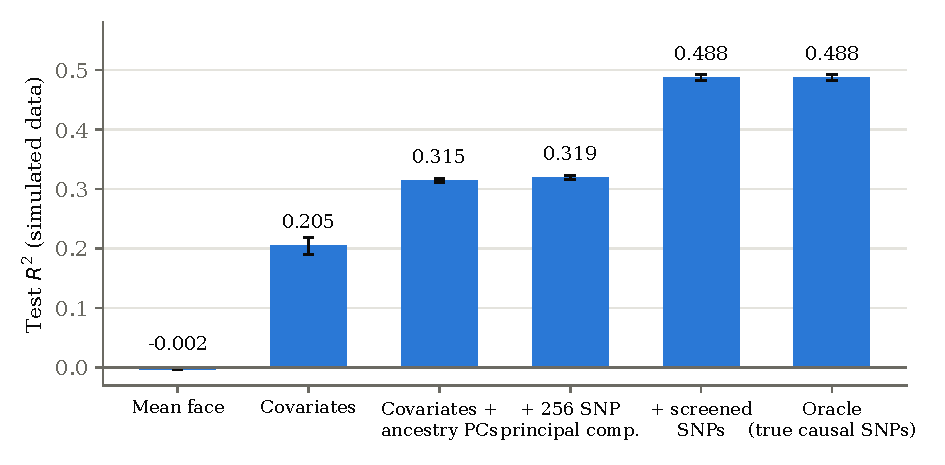
\includegraphics[width=0.86\textwidth]{Figures/res_ladder.pdf}
\caption{Baseline ladder on the matched simulated cohort. Error bars show the standard deviation over five generated cohorts.}
\label{fig:res-ladder}
\end{figure}

Three observations follow. First, ancestry components add 0.110 over the other covariates, which confirms that the simulated cohort contains the population structure it was designed to contain, and that a baseline without ancestry would flatter any genetic model. In the simulation, ten ancestry components estimated from genotype do as well as the true ancestry labels ($0.315$ against $0.316$), so the baseline does not depend on information that real data would lack.

Second, the oracle shows that SNPs can add $0.173$ beyond covariates and ancestry. A ridge regression on screened SNPs recovers all of it, with per-cohort confidence intervals lying between $+0.159$ and $+0.188$. The pipeline therefore finds the planted signal.

Third, the same SNPs passed through 256 principal components add only $0.004$. This matters because our first round of experiments used that representation alone, and on that basis we had provisionally concluded that SNPs added nothing beyond demographics. The oracle exposed that conclusion as an artefact of our own feature step. The leading components of unlinked SNPs capture ancestry, which the baseline already has, and discard the small individual effects that carry the planted signal. We report this openly, because the correction is the most useful methodological lesson of this phase: a null result is trustworthy only if a positive control shows that the method could have found an effect.

Table~\ref{tab:res-neg} reports the negative controls. When genotype rows are shuffled so that faces and genotypes no longer belong together, and when the cohort is regenerated with no genetic contribution, the gain from SNPs is $-0.001$ in both cases. The small negative value is expected, since fitting uninformative features costs a little accuracy. No confidence interval lies above zero. The pipeline therefore reports no signal where none exists, which rules out leakage between the training and test sets.

\begin{table}[!ht]
\centering
\caption{Positive and negative controls. Gain in test $R^2$ from adding screened SNPs to covariates and ancestry components.}
\label{tab:res-neg}
\small
\begin{tabular}{|p{8.6cm}|p{2.2cm}|p{3.5cm}|}
\hline
\textbf{Condition} & \textbf{Gain} & \textbf{Expected} \\ \hline
Planted genetic share of 0.20 (five cohorts) & $+0.173$ & clearly above zero \\ \hline
Genotype rows shuffled (five cohorts) & $-0.001$ & zero \\ \hline
Planted genetic share of zero (three cohorts) & $-0.001$ & zero \\ \hline
\end{tabular}
\end{table}

\section{Comparison of Models}
\label{sec:res-models}
With the pipeline validated, the four neural models were compared with the demographic baseline, each given the demographic covariates together with one of the two SNP representations of Section~\ref{sec:impl-features}. Table~\ref{tab:res-models} and Figure~\ref{fig:res-models} give the results.

\begin{table}[!ht]
\centering
\caption{Neural models on the matched simulated cohort. Test $R^2$, mean and standard deviation over three training runs. The demographic baseline scores $0.317$.}
\label{tab:res-models}
\small
\begin{tabular}{|p{4.6cm}|p{3.6cm}|p{3.1cm}|p{2.9cm}|}
\hline
\textbf{Model} & \textbf{256 SNP principal components} & \textbf{256 screened SNPs} & \textbf{Mesh error, screened (mm)} \\ \hline
Demographics only (baseline) & $0.317$ & $0.317$ & $3.00$ \\ \hline
Multilayer perceptron & $0.274 \pm 0.001$ & $0.396 \pm 0.002$ & $2.79$ \\ \hline
Contrastive model & $0.220 \pm 0.004$ & $0.364 \pm 0.001$ & $2.88$ \\ \hline
Transformer encoder & $0.311 \pm 0.005$ & $0.319 \pm 0.002$ & $3.00$ \\ \hline
Conditional diffusion & $-0.368 \pm 0.006$ & $0.081 \pm 0.006$ & $3.38$ \\ \hline
\end{tabular}
\end{table}

\begin{figure}[!ht]
\centering
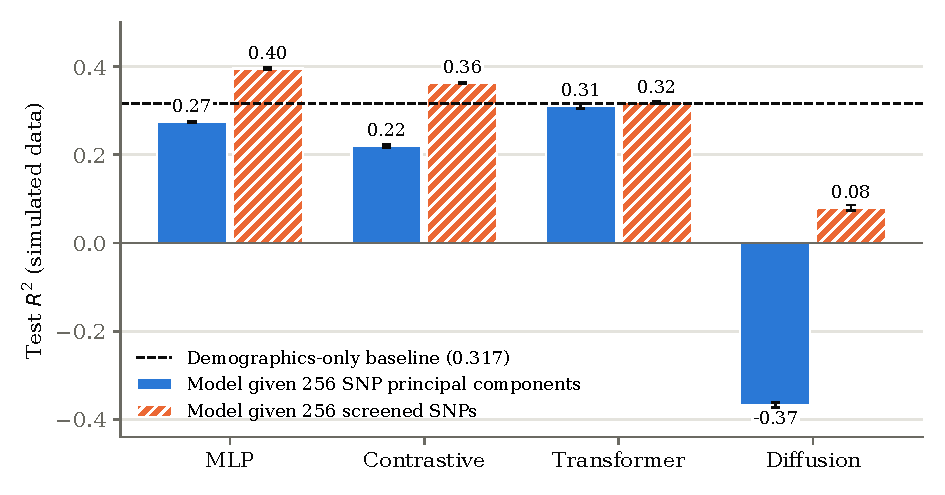
\includegraphics[width=0.86\textwidth]{Figures/res_models.pdf}
\caption{Neural models with two SNP representations, against the demographic baseline. Error bars show the standard deviation over three training runs.}
\label{fig:res-models}
\end{figure}

With principal components, no neural model exceeds the demographic baseline, which agrees with the finding of Section~\ref{sec:res-controls} that this representation carries almost no usable genetic signal. With screened SNPs, the multilayer perceptron and the contrastive model both exceed the baseline clearly, by $0.079$ and $0.047$. The mean mesh error of the multilayer perceptron falls from $3.00$ to $2.79$ millimetres. The Transformer stays at the baseline, and the diffusion model remains far below it, although it improves greatly over its result with principal components.

The choice of SNP representation therefore mattered more than the choice of architecture. The same multilayer perceptron moves from below the baseline to well above it when only its input changes.

The comparison with the linear reference is the central result for the question of model complexity. The best neural model recovers $0.079$ of the $0.173$ that is available, less than half, while the tuned ridge regression of Table~\ref{tab:res-ladder} recovers all of it. The two figures come from different scripts, and the ridge regression was tuned over the number of SNPs while the neural models were given a fixed 256, so the comparison is indicative and not exact. The gap of about $0.09$ is nevertheless far larger than any difference that this could explain. This result must be read with the design of the simulation in mind. The planted effects are linear and additive, so a linear model is the correctly specified one. The experiment shows that the neural models are less efficient at learning a linear signal from about two thousand subjects. It does not show that neural models are worse in general, and it cannot show whether real facial genetics contains non-linear structure that would favour them.

The shuffled-genotype control was also applied to the neural models, with one training run each. The Transformer scored $0.316$, the multilayer perceptron $0.252$, and the contrastive model $0.247$, against $0.317$ for the baseline. No model gains from uninformative SNPs, which again rules out leakage. Two further points follow. The multilayer perceptron and the contrastive model lose about $0.07$ when given uninformative SNPs, so on data with very weak genetic signal they could fall below the demographic baseline. The Transformer scores the same with shuffled and with real genotypes, which indicates that at this sample size it is not using the SNPs at all.

\section{Effect of Sample Size}
To ask whether more subjects would change these conclusions, a separate cohort of 10{,}000 subjects was generated with the same settings. Models were trained on nested subsets of its training set and scored on one fixed test set of 1{,}500 subjects. This is a scaling experiment only. The real cohort has 3{,}118 subjects, so results beyond the first row of Table~\ref{tab:res-scaling} describe a cohort that we will not have.

\begin{table}[!ht]
\centering
\caption{Effect of training-set size, with screened SNPs. Test $R^2$, mean over three training runs. Standard deviations are at most $0.003$ except for the diffusion model, where they reach $0.012$.}
\label{tab:res-scaling}
\small
\begin{tabular}{|p{2.5cm}|p{2.4cm}|p{2.0cm}|p{2.2cm}|p{2.3cm}|p{1.9cm}|}
\hline
\textbf{Training subjects} & \textbf{Demographics} & \textbf{Multilayer perceptron} & \textbf{Contrastive} & \textbf{Transformer} & \textbf{Diffusion} \\ \hline
2{,}182 & $0.312$ & $0.389$ & $0.349$ & $0.310$ & $0.058$ \\ \hline
4{,}000 & $0.313$ & $0.417$ & $0.392$ & $0.316$ & $0.049$ \\ \hline
7{,}000 & $0.314$ & $0.435$ & $0.428$ & $0.338$ & $0.028$ \\ \hline
\end{tabular}
\end{table}

\begin{figure}[!ht]
\centering
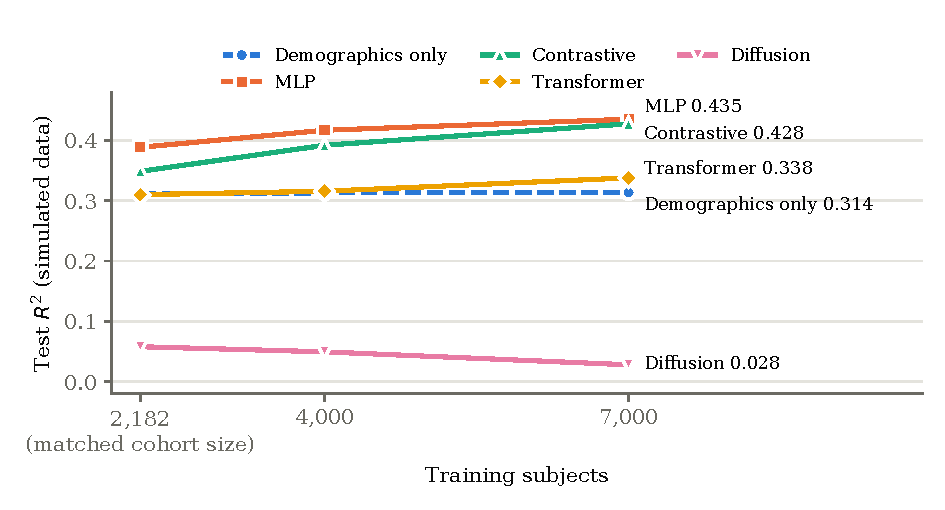
\includegraphics[width=0.86\textwidth]{Figures/res_scaling.pdf}
\caption{Effect of training-set size on each model, with screened SNPs.}
\label{fig:res-scaling}
\end{figure}

The demographic baseline is flat, as expected for a linear model with a handful of inputs. The multilayer perceptron gains $0.046$ and the contrastive model $0.079$ from roughly three times the data, and the contrastive model nearly closes its gap to the multilayer perceptron. The Transformer begins to exceed the baseline only at 7{,}000 subjects. The diffusion model does not improve with more data. We have not diagnosed the cause, and we report it as an open negative result.

Table~\ref{tab:res-power} gives a companion analysis with the linear screen, over cohort sizes and planted genetic shares. At the size of the real cohort, SNPs add $0.070$ when the planted share is 0.10 and $0.177$ when it is 0.20, and nothing when it is zero. These figures are an optimistic upper bound and not a forecast for real data, for the reasons given in Section~\ref{sec:res-limits}.

\begin{table}[!ht]
\centering
\caption{Gain in test $R^2$ from screened SNPs, by cohort size and planted genetic share. Mean of two generated cohorts.}
\label{tab:res-power}
\small
\begin{tabular}{|p{3.2cm}|p{3.0cm}|p{3.0cm}|p{3.0cm}|}
\hline
\textbf{Cohort size} & \textbf{Share 0.00} & \textbf{Share 0.10} & \textbf{Share 0.20} \\ \hline
1{,}000 & $-0.000$ & $+0.022$ & $+0.119$ \\ \hline
2{,}000 & $-0.001$ & $+0.055$ & $+0.157$ \\ \hline
3{,}118 & $-0.001$ & $+0.070$ & $+0.177$ \\ \hline
6{,}000 & $-0.001$ & $+0.087$ & $+0.192$ \\ \hline
\end{tabular}
\end{table}

\section{Recovery of Published Associations}
Section~\ref{sec:impl-inject} described how 14 published associations between lead SNPs and facial measurements were added to the simulated measurements. To check that the evaluation can recover known associations and only those, every one of the 260 pairs of SNP and measurement was tested after adjusting both for sex, age, age squared, height, weight, and ancestry. All 14 injected pairs were detected at a Bonferroni threshold, each with the published direction of effect. None of the 246 pairs that were not injected was detected, and 2.8 per cent of them fell below 0.05, which is consistent with chance. On the larger cohort of 10{,}000 subjects the result was the same, with 6.1 per cent of the remaining pairs below 0.05.

This result confirms that the association machinery is correct and that adjustment for ancestry prevents false associations in a structured cohort. It is not a replication of the published associations. The signals were placed in the data by us, so finding them shows that the method works and nothing more.

\section{Appearance Integration}
\label{sec:res-app-sim}
The appearance module was applied to the 41 marker SNPs of every subject in the matched simulated cohort. Table~\ref{tab:res-app} gives the distribution of the predicted categories.

\begin{table}[!ht]
\centering
\caption{Predicted appearance categories on the matched simulated cohort, as a percentage of subjects. These describe the simulation only.}
\label{tab:res-app}
\small
\begin{tabular}{|p{2.6cm}|p{11.6cm}|}
\hline
\textbf{Trait} & \textbf{Predicted categories} \\ \hline
Eye colour & blue 54.7, brown 44.1, intermediate 1.2 \\ \hline
Hair colour & brown 68.8, blond 17.9, red 8.6, black 4.7 \\ \hline
Hair shade & light 63.0, dark 37.0 \\ \hline
Skin colour & intermediate 72.5, pale 14.0, very pale 12.2, dark to black 1.1, dark 0.3 \\ \hline
\end{tabular}
\end{table}

These figures show that the module runs end to end on the same genotype file as the shape models and returns a varied and plausible mix of categories, which is what RQ8 asks of the integration. They are not a measure of accuracy. The marker frequencies in the simulation are synthetic and the cohort has no colour labels to compare against.

\subsection{Why the Colour Component Was Not Tested on Real People}
\label{sec:res-appearance-untested}
Colour is the one part of FaceCon that could in principle have been checked against real human phenotypes, because the model is a published one that this project did not fit, and because self-reported eye colour is the kind of label an open cohort might carry. The check was written: it maps survey answers onto the model's three categories, scores one-against-rest areas under the curve, and compares them against a null built from a thousand label shuffles. It was validated end to end on a stand-in cohort, where it proved sensitive to the direction of the labels, scoring $0.995$ with them correctly oriented and $0.000$ reversed, with the shuffled null centred on one half as it should be.

It was never run, because the data source stopped serving. The intended cohort was the Harvard Personal Genome Project, whose participants publish genotype files and trait surveys under a public-domain dedication, making it usable without an access application. Its site now answers every request with a redirect to the identical address, over both plain and encrypted connections and regardless of the client, which no client can resolve; a separate fault leaves its certificate valid only for a hostname that forwards to the one that loops. The other candidate, openSNP, which paired consumer genotypes with self-reported traits, shut down permanently in April 2025 and deleted its data.

This is worth stating as more than an inconvenience. The open genotype-and-phenotype resources on which an independent check of a published appearance model depends have largely ceased to exist, and a project without institutional data access has no remaining route to one. FaceCon therefore reports its colour component as integrated and faithful to the official calculator, and makes no claim whatever about its accuracy on real people. That silence is not a choice of scope: it is the honest consequence of there being nothing left to test against.

\section{Experiments on Real Genotypes}
\label{sec:res-real}
The experiments reported so far use genotypes that we generated ourselves, and Section~\ref{sec:res-limits} identifies three ways in which such genotypes are easier than real ones. They are statistically independent of one another, whereas real SNPs that sit close together on a chromosome are correlated. Their allele frequencies are drawn from a convenient range. Their ancestry groups are cleanly separated, whereas real population structure is continuous. To remove these three advantages, the experiment was repeated with real human genotypes in place of simulated ones, using the panel described in Section~\ref{sec:impl-1kg}. The faces remain simulated, so this experiment is still not a statement about real faces. What changes is that the genotype side of the problem is now real.

The cohort holds 2{,}573 unrelated people from the 1000 Genomes Project and 100{,}009 SNPs, divided into 1{,}801 training, 385 validation, and 387 test subjects. The five continental groups are unevenly represented, with 680 African, 525 European, 511 South Asian, 506 East Asian, and 351 American subjects, which is itself more realistic than the balanced groups of the simulation. The planted genetic share is again 0.20, but the effects are now sparse, with 300 causal SNPs each affecting 5 of the 50 shape dimensions rather than all of them. Table~\ref{tab:res-kg-ladder} gives the baseline ladder, and the left panel of Figure~\ref{fig:res-kg} shows what SNPs add.

\begin{table}[!ht]
\centering
\caption{Baseline ladder on real genotypes with simulated faces. Test $R^2$, mean and standard deviation over five generated cohorts.}
\label{tab:res-kg-ladder}
\small
\begin{tabular}{|p{8.4cm}|p{2.6cm}|p{3.3cm}|}
\hline
\textbf{Model} & \textbf{Test $R^2$} & \textbf{Gain over row 3} \\ \hline
1. Mean face & $-0.003 \pm 0.000$ & --- \\ \hline
2. Covariates (sex, age, age squared, height, weight) & $0.195 \pm 0.010$ & --- \\ \hline
3. Covariates and ten ancestry principal components & $0.335 \pm 0.008$ & reference \\ \hline
4. Row 3 and 256 SNP principal components & $0.335 \pm 0.009$ & $+0.001$ \\ \hline
5. Row 3 and screened SNPs (ridge regression) & $0.435 \pm 0.006$ & $+0.100$ \\ \hline
6. Row 3 and the true causal SNPs (oracle) & $0.449 \pm 0.005$ & $+0.114$ \\ \hline
\end{tabular}
\end{table}

The pattern of Section~\ref{sec:res-controls} survives the change of genotypes, with two differences worth recording. The oracle now adds $0.114$ and the screen recovers $0.100$ of it, which is 88 per cent rather than all of it. Real correlation between SNPs makes the causal ones harder to isolate, which is the expected direction. The 256 principal components add $0.001$, which is zero to the precision that matters, so the finding that this representation discards the genetic signal is not an artefact of unlinked simulated SNPs. A second difference appears one row higher. True ancestry labels score $0.345$ against $0.335$ for ten estimated components, a gap that was absent in the simulation, which is what continuous population structure should do to a fixed number of components.

\begin{figure}[!ht]
\centering
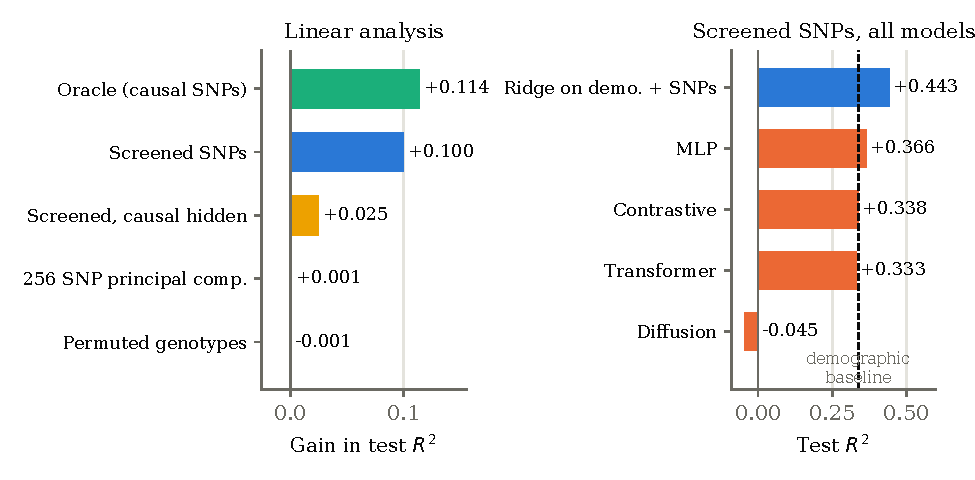
\includegraphics[width=0.92\textwidth]{Figures/res_kg.pdf}
\caption{Real genotypes with simulated faces. The left panel shows what SNPs add beyond covariates and ancestry components. The right panel compares the models with the linear reference on the same split.}
\label{fig:res-kg}
\end{figure}

\subsection{What Correlation Between SNPs Carries}
\label{sec:res-ld}
Real genotypes make a question possible that the simulation could not pose. In a real study the causal variant is usually not on the array, and an association is detected only because a nearby SNP is correlated with it. To measure how much of the signal survives that indirection, the analysis was repeated with the 300 causal SNPs deleted from the panel, so that no model could use them and only their neighbours remained.

Under this condition the screen adds $0.025$, against $0.114$ when the causal SNPs are available. Correlation between neighbouring SNPs therefore carries about 22 per cent of the available signal. The per-cohort confidence intervals lie between $+0.018$ and $+0.035$ and none includes zero, so the effect is real rather than noise. The same experiment on the simulated panel of Section~\ref{sec:res-controls} gives $-0.001$, as it must, because unlinked SNPs have no neighbours to carry anything. This is the clearest illustration in this report of why the realism of the genotype matters, and it offers a mechanism for an observation that is common in the published literature, namely that individual associated SNPs explain very little variance. A panel of common SNPs reads neighbours and not causes, and a fifth of the attainable signal is what that indirection leaves.

\subsection{Models Against the Linear Reference}
Table~\ref{tab:res-kg-models} compares the four neural models with two linear references on the same cohort and the same split. The first reference uses the demographic covariates alone. The second is given exactly what the neural models are given, which is the covariates together with the SNP features, and is fitted in two stages so that the covariates are not penalised. This second reference did not exist for the experiments of Section~\ref{sec:res-models}, where the linear and neural results came from different scripts and could only be compared indirectly. Here the comparison is exact.

\begin{table}[!ht]
\centering
\caption{Models on real genotypes with simulated faces. Test $R^2$, mean and standard deviation over three training runs. The linear references are fitted once and have no spread, and the permuted column is a single run of each model.}
\label{tab:res-kg-models}
\small
\begin{tabular}{|p{5.4cm}|p{3.4cm}|p{3.0cm}|p{2.2cm}|}
\hline
\textbf{Model} & \textbf{256 SNP principal components} & \textbf{256 screened SNPs} & \textbf{Permuted genotypes} \\ \hline
Demographics only (baseline) & $0.338$ & $0.338$ & $0.338$ \\ \hline
Ridge on demographics and SNPs & $0.338$ & $0.443$ & $0.338$ \\ \hline
Multilayer perceptron & $0.242 \pm 0.002$ & $0.366 \pm 0.001$ & $0.243$ \\ \hline
Transformer encoder & $0.327 \pm 0.001$ & $0.333 \pm 0.001$ & $0.330$ \\ \hline
Contrastive model & $0.175 \pm 0.002$ & $0.338 \pm 0.002$ & $0.239$ \\ \hline
Conditional diffusion & $-0.523 \pm 0.034$ & $-0.045 \pm 0.014$ & $-0.291$ \\ \hline
\end{tabular}
\end{table}

The linear reference adds $0.106$ over the demographic baseline. The baseline ladder of Table~\ref{tab:res-kg-ladder} measures a closely related quantity with separate fitting and scoring code, ten ancestry components in place of ancestry labels, and a number of SNPs tuned on the validation set rather than a fixed 256. The first of its five cohorts is the cohort used here, with the same subjects and the same split, and on it the controls script reports a gain of $0.105$. Two implementations that differ in all of these respects agreeing to within $0.001$ on the same subjects is the strongest evidence available to us that neither contains an error in the direction that matters. Averaged over all five cohorts, the gain is $0.100$.

The best neural model adds $0.028$, which is a quarter of what the linear reference adds and a quarter of what the oracle makes available. The gap between the best neural model and the linear reference is $0.077$ on the same split. Only the multilayer perceptron responds to the genotypes at all. The Transformer scores $0.333$ with real SNPs and $0.330$ with permuted ones, a difference within its run-to-run spread, so it is reading the covariates and ignoring the genotypes. The contrastive model lands exactly on the demographic baseline. The diffusion model remains below the mean face and is worse here than on the simulated panel.

With principal components, every neural model falls at or below the demographic baseline, and the linear reference given the same features scores exactly the baseline value. When a correctly specified linear model extracts nothing from a representation, the representation contains nothing to extract, and the failure of the neural models on these features cannot be attributed to the models.

\subsection{Controls on the Real Panel}
Both negative controls were repeated. With genotype rows shuffled, the linear reference scores $0.338$, which is the demographic baseline to three decimal places, and every neural model scores at or below it. The acceptance check that no model gains more than $0.01$ over the baseline passes for the neural models and for the linear reference.

The second of these checks was added after an error of our own. The linear reference was first written as a single ridge regression over the covariates and the SNP features together, which penalises the covariates alongside the SNPs. On permuted genotypes that version scored $0.207$ against a baseline of $0.317$, because the large penalty that uninformative features require also shrinks the covariates that carry real information. It would have understated the linear option precisely where the comparison with the neural models is strictest. The two-stage form used in Table~\ref{tab:res-kg-models} fits the covariates without penalty and then fits the SNP features to what the covariates leave over, and returns the baseline value exactly under permutation. The check is now part of the suite so that the error cannot return unnoticed.

The association analysis of Section~\ref{sec:impl-inject} was also repeated on the real panel. All 14 injected associations were recovered with the published direction, no Bonferroni detection appeared among the 246 pairs that were not injected, and 6.1 per cent of them fell below 0.05. Real correlation between SNPs did not create false associations once ancestry was adjusted for.

The frequency check described in Section~\ref{sec:impl-1kg} flagged 2 of the 13 published lead SNPs, whose frequency in the European subjects of the panel differs from the published one by more than the tolerance. Both are insertions or deletions, for which the identifier in the 1000 Genomes files refers to a different representation of the variant than the published table does. Neither reached genome-wide significance in the source study, and both carry weights that we planted rather than published ones, so no result in this chapter depends on their alignment. They are reported because the check exists in order to be acted on rather than passed over.

\subsection{Appearance on Real Genotypes}
The appearance module was applied to the real marker genotypes of the same people. Of the 41 markers, 39 are present in the panel. The two that are absent, N29insA and Y152OCH, are rare variants of the MC1R gene associated with red hair, and treating every subject as a non-carrier of them will understate red hair. Table~\ref{tab:res-kg-app} gives the most frequent predicted category for each trait and group.

\begin{table}[!ht]
\centering
\caption{Most frequent predicted appearance category by continental group, on real marker genotypes, as a percentage of subjects in the group. These are plausibility checks and not measures of accuracy.}
\label{tab:res-kg-app}
\small
\begin{tabular}{|p{2.9cm}|p{3.7cm}|p{3.5cm}|p{3.9cm}|}
\hline
\textbf{Group} & \textbf{Eye colour} & \textbf{Hair colour} & \textbf{Skin colour} \\ \hline
African & brown 99.7 & black 94.1 & dark to black 99.1 \\ \hline
East Asian & brown 100.0 & black 100.0 & dark to black 89.5 \\ \hline
South Asian & brown 99.8 & black 82.0 & dark to black 52.6 \\ \hline
American & brown 94.3 & black 49.6 & dark to black 40.5 \\ \hline
European & brown 52.0 & brown 57.1 & intermediate 89.9 \\ \hline
\end{tabular}
\end{table}

The predictions vary between groups in the direction that the published model predicts, with blue eyes and lighter skin far more frequent among Europeans than among the other groups. This is a stronger check than the one in Section~\ref{sec:res-app-sim}, because the marker genotypes are real rather than simulated. It remains a plausibility check and not an accuracy measurement, since the 1000 Genomes Project records no eye, hair, or skin colour for its subjects, so there is nothing to compare the predictions against.

\subsection{What This Experiment Does and Does Not Establish}
Three of the advantages that the simulation gave the method have been removed, and the main conclusions survive. SNPs add a measurable amount beyond covariates and ancestry, principal components discard that signal, the pipeline stays silent under permutation, and a regularised linear model beats every neural model. Two new results appear, namely that correlation between SNPs carries about a fifth of the attainable signal, and that the gap between neural and linear models is $0.077$ when both are given identical inputs on one split.

The limits of the experiment should be equally clear. The faces, ages, heights, and weights are still simulated, and the mapping from genotype to face is one we imposed. That mapping is additive and linear, so the linear reference is the correctly specified model and is expected to win. The result shows that these neural models are inefficient at learning an additive signal from 1{,}801 training subjects, and it cannot show how they would behave on a signal with the non-linear structure that real facial genetics may or may not contain. The planted share of 0.20 is a design choice and not an estimate of the real one. For these reasons the figures in this section remain properties of the pipeline rather than facts about human faces.

\section{When the Signal Is Not Additive}
\label{sec:res-nonadd}
Every experiment reported so far planted an additive signal, in which each copy of an allele shifts the face by the same amount and no SNP depends on another. Section~\ref{sec:res-limits} lists that as a limitation: the linear reference is the correctly specified model for such a signal, so its victory over the neural models says nothing about a signal with structure. Real facial genetics may contain dominance, where the heterozygote does not sit midway between the two homozygotes, and epistasis, where the effect of one SNP depends on the genotype at another. Neither can be measured from data the project does not have. What can be done is to plant them deliberately and ask what the evaluation sees.

Four further cohorts were generated, identical to the matched cohort in every other respect, differing only in how the planted genetic share of 0.20 is divided. In the dominance cohort half of that share is carried by heterozygote deviations; in the epistasis cohort half is carried by products of pairs of centred genotypes; in the mixed cohort a third goes to each. The additive cohort is the original. Two rows were added to the ladder for these cohorts. The first, written \mbox{+SNP-screen-NA}, replaces the single additive screen with a two-degree-of-freedom score that tests each SNP's additive and heterozygote terms together and keeps both columns for the SNPs it selects. The second, ORACLE-NA, is given the true causal SNPs, the true heterozygote codes, and the true interacting pairs. Table~\ref{tab:res-nonadd} reports the gain of each row over the \mbox{cov+PC} baseline, averaged over the same five cohorts used throughout.

\begin{table}[!ht]
\centering
\caption{Gain in $R^2$ over the covariates-and-components baseline when the planted signal is not additive. Five cohorts per arm. The calibration arm is the same additive cohort with the two extra rows also fitted, which is what makes the cost of those rows visible. All faces are simulated and the architecture is one we imposed.}
\label{tab:res-nonadd}
\small\setstretch{1.15}
\begin{tabular}{|p{3.3cm}|p{2.0cm}|p{2.0cm}|p{2.0cm}|p{2.0cm}|p{1.9cm}|}
\hline
\textbf{Row} & \textbf{Additive} & \textbf{Calibration} & \textbf{Dominance} & \textbf{Epistasis} & \textbf{Mixed} \\ \hline
+SNP-screen    & $+0.1726$ & $+0.1726$ & $+0.0987$ & $+0.0699$ & $+0.0565$ \\ \hline
+SNP-screen-NA & ---       & $+0.1501$ & $+0.1536$ & $+0.0523$ & $+0.0884$ \\ \hline
ORACLE         & $+0.1729$ & $+0.1729$ & $+0.0987$ & $+0.0717$ & $+0.0581$ \\ \hline
ORACLE-NA      & ---       & $+0.1429$ & $+0.1451$ & $+0.1475$ & $+0.1477$ \\ \hline
Permuted genotypes & $-0.0006$ & $-0.0006$ & $-0.0007$ & $-0.0007$ & $-0.0007$ \\ \hline
Zero genetic share & $-0.0011$ & $-0.0011$ & $-0.0011$ & $-0.0011$ & $-0.0011$ \\ \hline
\end{tabular}
\end{table}

\begin{figure}[!ht]
\centering
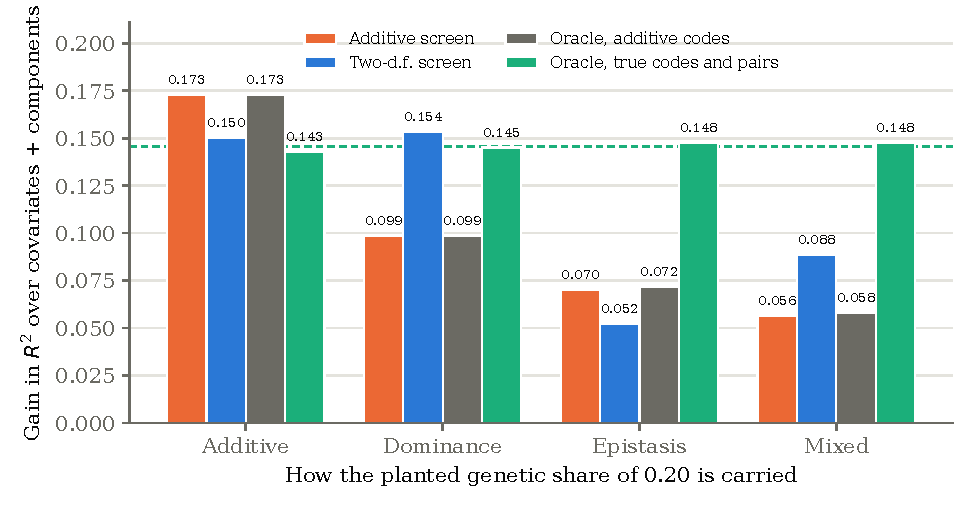
\includegraphics[width=\textwidth]{Figures/res_nonadd.pdf}
\caption{What each model recovers as the form of the planted signal changes, while its total size stays at 0.20. The dashed line marks the mean of the oracle given the true codes and pairs, which is nearly flat across all four architectures; the additive models fall away from it. Simulated faces, imposed architecture.}
\label{fig:res-nonadd}
\end{figure}

The last two rows come first, because without them the rest would not be interpretable. Permuting the genotypes and setting the genetic share to zero both return approximately zero in every arm, so the extra rows have not introduced a way of finding signal that is not there.

The main result, drawn in Figure~\ref{fig:res-nonadd}, is in the ORACLE-NA row. Given the right representation, the recoverable signal is almost the same in all four arms, between $0.143$ and $0.148$, which is what should happen: the same total share of 0.20 was planted each time and only its form was changed. The additive oracle, by contrast, falls from $0.173$ on the additive cohort to $0.058$ on the mixed one. A model restricted to additive allele dosages therefore sees about a third of a signal that is in fact fully present in the genotypes. This is the clearest statement this project can make about why published association studies report small individual effects: part of the shortfall need not be absent signal at all, but signal in a form that the standard additive model cannot express.

The practical rows behave less tidily, and in one case worse than the additive row they were meant to improve on. On the dominance cohort the two-degree-of-freedom screen gains $0.1536$ against the additive screen's $0.0987$, and on the mixed cohort $0.0884$ against $0.0565$. On the epistasis cohort it gains $0.0523$ against $0.0699$, which is to say it is worse than doing nothing. This was not expected, and Section~\ref{sec:res-nonadd-honest} sets out why it happens and what was and was not done about it.

\subsection{Two Expectations That Were Wrong}
\label{sec:res-nonadd-honest}
This experiment was pre-registered before any of its numbers were read, with the thresholds and the expected direction of each row written down in advance. Two of those expectations turned out to be wrong, and both are recorded here rather than quietly corrected, because a protocol that is only reported when it agrees with the result is not a protocol.

The first concerns the cost of the extra rows. Fitting dominance and interaction columns on a cohort where they carry nothing cannot help, and was expected to cost about $0.02$ in $R^2$. The measured cost is larger: ORACLE sits $0.030$ above ORACLE-NA on the additive-calibration arm averaged over five cohorts, and $0.032$ on a single cohort. The pre-registered figure was not loosened to accommodate this. The consequence matters for reading Table~\ref{tab:res-nonadd}: ORACLE-NA is not a drop-in replacement for ORACLE, the two are comparable only within an arm, and the fact that ORACLE-NA is the lower of the two on the additive cohort is the expected direction and not a failure. Because the cost is of the same order as some of the gains in the table, it has to be stated plainly; a reader comparing ORACLE-NA on the mixed cohort against ORACLE on the additive one would otherwise read a modelling cost as a loss of signal.

The second concerns the epistasis cohort. The screen was expected to beat the additive screen wherever the signal was not additive, and it does not. The reason is a property of the screen and not a fault in the data: its per-SNP score tests a genotype's own heterozygote deviation, so it has power against dominance and none against a product of two SNPs whose individual effects average out. On that cohort the extra column per SNP is noise, and it costs what the paragraph above measures. The pre-registered expectation was wrong to treat non-additive as a single case. That the signal is nonetheless there is settled by ORACLE-NA, which recovers $0.1475$ on the same cohort when it is told which pairs interact; what fails is finding the pairs, not representing them.

No pair-aware screen was added in response. Designing a method after seeing which cohort defeated the existing one, and then reporting its success on that same cohort, would produce a number that means nothing. A screen over candidate pairs is named as future work in Chapter~\ref{ch:conclusion}, to be specified before it is run.

\subsection{The Neural Models on Non-Additive Signal}
\label{sec:res-nonadd-neural}
Chapter~\ref{ch:results} has so far reported that the regularised linear model beats every neural model, with the caveat that the planted signal was additive and the linear model was therefore correctly specified. The cohorts of Section~\ref{sec:res-nonadd} remove that caveat: a third of the genetic share is carried by heterozygote deviations and a third by interactions between pairs, so the linear model on additive dosages is now the wrong model, and the comparison is one the neural models should be expected to win. The pre-registered primary comparison is the best neural model minus the ridge on demographics and SNPs, on the two-degree-of-freedom features, paired within each of three independently generated cohorts.

\begin{table}[!ht]
\centering
\caption{Test parameter $R^2$ on the mixed-architecture cohorts, mean and standard deviation over three independently generated cohorts. The gap is the best neural model minus the ridge, paired within cohort, with a $t$ interval over the three.}
\label{tab:res-nonadd-neural}
\small\setstretch{1.15}
\begin{tabular}{|p{3.1cm}|p{2.3cm}|p{2.3cm}|p{2.0cm}|p{2.2cm}|p{2.6cm}|}
\hline
\textbf{Features} & \textbf{Demographics} & \textbf{Ridge, demo.\ + SNP} & \textbf{MLP} & \textbf{Transformer} & \textbf{Gap, best neural $-$ ridge} \\ \hline
Additive screen & $+0.307$ & $+0.344$ & $+0.294$ & $+0.306$ & $-0.038$ $[-0.050,-0.027]$ \\ \hline
Two-d.f.\ screen & $+0.307$ & $+0.391$ & $+0.326$ & $+0.306$ & $-0.065$ $[-0.070,-0.061]$ \\ \hline
Permuted control & $+0.308$ & $+0.308$ & $+0.251$ & $+0.304$ & --- \\ \hline
\end{tabular}
\end{table}

The ridge wins, and it wins by more than it did on additive signal. The gap is $-0.065$ with an interval that excludes zero comfortably, and it is wider on the two-degree-of-freedom features than on the additive ones. Removing the linear model's home advantage did not close the gap; it widened it. All four permuted negative controls pass, so none of this is an artefact of the models finding structure that is not there.

What separates the models is what each does with the better representation. Given the two-degree-of-freedom features in place of additive dosages, the ridge gains $0.047$, the MLP gains $0.032$, and the transformer gains nothing at all. The transformer is in fact the more striking case: at $+0.306$ it sits a thousandth below the demographics-only baseline on both feature sets, and it scores the same when the genotypes are permuted as when they are real. On this data, at this sample size, it is extracting no usable information from the genotypes whatsoever, and its apparent competence is entirely the covariates. The MLP does use the SNPs, since permuting them costs it $0.075$, but on additive features it still finishes $0.013$ below a model given only demographics, which is to say the SNP information it extracts does not pay for the overfitting it incurs.

The honest conclusion is narrow and should not be stretched. These two architectures, at this sample size, on these cohorts, cannot exploit non-additive structure that a linear model recovers from the same features. That is a statement about $n \approx 2{,}200$ training subjects and two specific architectures, not about neural networks and genetics in general; the published results that motivate such models use cohorts one to two orders of magnitude larger. What this project can say is that scale, not architecture, is the first thing to change, and that on a cohort of the size FaceCon expects, the representation handed to a regularised linear model matters more than the choice of network.

\section{Where the Gain Falls, and on Whom}
\label{sec:res-regional}
The results so far report one number for the whole face. Two questions ask for more detail. RQ6 asks whether some parts of the face are predicted better than others, and RQ7 asks whether the prediction works equally well for every ancestry group. Both were run on the real-genotype cohort, comparing the ridge model on covariates and screened SNPs against the demographic baseline, with confidence intervals from 2{,}000 bootstrap resamples of the test subjects.

\begin{table}[!ht]
\centering
\caption{Reduction in mean vertex error, in millimetres, from adding SNPs to the demographic baseline, by facial region and by ancestry group. Positive means the SNP model is closer to the simulated truth. Relative is the reduction as a percentage of the baseline error for that region.}
\label{tab:res-regional}
\small\setstretch{1.15}
\begin{tabular}{|p{3.4cm}|p{2.6cm}|p{2.4cm}|p{5.2cm}|}
\hline
\textbf{Region or group} & \textbf{Gain (mm)} & \textbf{Relative} & \textbf{Note} \\ \hline
Whole head & $0.356$ & $13.5$ per cent & 95 per cent interval $0.305$ to $0.408$ \\ \hline
Jaw & $0.567$ & $14$ per cent & largest absolute gain \\ \hline
Cheeks & $0.485$ & $14$ per cent & \\ \hline
Forehead & $0.337$ & $14$ per cent & \\ \hline
Mouth & $0.304$ & $14$ per cent & \\ \hline
Nose & $0.213$ & $13$ per cent & \\ \hline
Eyes & $0.203$ & $13$ per cent & smallest absolute gain \\ \hline
African group & $0.332$ & --- & intervals overlap \\ \hline
European group & $0.388$ & --- & intervals overlap \\ \hline
Other groups & $0.347$ & --- & intervals overlap \\ \hline
\end{tabular}
\end{table}

The absolute gains differ by a factor of nearly three between the jaw and the eyes, and it would be easy to present that as a finding about facial genetics. It is not one. In relative terms the gains are flat, between 13 and 14 per cent of the baseline error in every region, and the ordering of the absolute gains is simply the ordering of how much the regions vary in the first place. That is exactly what a signal planted uniformly across all 50 shape dimensions should produce, and it is what was planted. The honest reading is that this analysis confirms the regional measurement works and shows no region to be preferentially predictable. A real regional difference, if one exists, is not something this cohort can contain.

Two finer checks point the same way. Every one of the 68 landmarks improves, and so does every one of the 50 shape dimensions, with no dimension made worse by adding SNPs. A planted global effect predicts precisely that, and a real signal concentrated in a few features would not.

The same analysis on the 1000 Genomes cohort, where the genotypes are real and correlated, gives a smaller overall gain of $0.231$ mm $[0.188, 0.271]$ and the same flat profile: between $6.7$ and $8.6$ per cent of the baseline error across the six regions, against $13$ to $14$ per cent on the simulated panel. The ordering of the regions is nearly unchanged, with the forehead and mouth swapping places, which is the kind of movement a difference of this size should produce by chance. Again all 68 landmarks and all 50 dimensions improve. The MLP, run on the same cohort for comparison, gains $0.046$ mm with an interval of $[-0.008, 0.100]$ that includes zero, and improves only 54 of 68 landmarks and 34 of 50 dimensions, which is consistent with Section~\ref{sec:res-nonadd-neural}.

\subsection{What the Subgroup Result Does and Does Not Establish}
\label{sec:res-fairness}
On the 1000 Genomes cohort the five continental groups gain $0.186$ mm (AFR, $n=108$), $0.223$ (AMR, $n=55$), $0.268$ (EAS, $n=80$), $0.237$ (EUR, $n=68$) and $0.257$ (SAS, $n=76$). All five confidence intervals share the common range $[0.194, 0.260]$, so no difference between any pair can be claimed from this data.

That sentence is easy to misread, and the misreading matters more here than anywhere else in this report. Overlapping intervals at these sample sizes are not evidence that the groups are predicted equally well. The groups number between 55 and 108 test subjects, the intervals are correspondingly wide, and a real difference of the size seen in the point estimates would not be detected reliably at this $n$. The lowest point estimate is the African group's, which is $0.082$ mm or about a third below the highest, and that is the direction a reader should be most alert to: African-ancestry cohorts carry more genetic diversity and shorter linkage blocks, so a screen selected on a pooled cohort has a specific reason to transfer to them less well. Nothing here establishes that this happened, and nothing here rules it out.

The limitation stands as stated earlier. Equal performance across groups is the expected outcome for cohorts carrying identical planted effects, and a method that passed this check could still fail badly on real faces. A fairness evaluation worth the name needs real scans, groups large enough to detect a difference that matters, and a threshold for what counts as an unacceptable gap fixed before the numbers are seen. This project provides none of those, and Chapter~\ref{ch:conclusion} keeps the question open rather than recording it as passed.

For RQ7 on the simulated panel the three group gains lie within $0.056$ mm of each other and their confidence intervals overlap, so no difference between groups is claimed. This is a weaker result than it appears: the groups were generated with the same planted effects and differ only in allele frequencies and sample size, so equal performance is the expected outcome and not evidence that the method would be fair on real data. Fairness across ancestry groups on real faces remains untested, and Chapter~\ref{ch:conclusion} keeps it as a requirement rather than a resolved question.

\section{Fitting the Face Model to Scans}
\label{sec:res-flame}
When the 3DFN scans arrive, each one must be converted into the 50-number shape vector that the models predict, by fitting the face model to the scan. That step cannot be tested on real scans yet, but it can be tested on synthetic ones, where the answer is known: a face is generated from a known shape vector, posed at a random rotation and translation, reduced to its surface points and 68 landmarks, and handed to the fitter without its shape vector. The fitter should return the vector it was built from.

Over 12 such scans the mean vertex error is $0.498$ mm with no noise added, and the worst of the 12 is $0.669$ mm, against a pre-registered bound of $1.0$ mm. Adding half a millimetre of noise to the surface points and one and a half millimetres to the landmarks raises the error to $0.609$ mm, so the procedure degrades gracefully rather than collapsing. The closed-form landmark stage alone reaches $1.044$ mm, so the iterative surface stage that follows it is doing real work.

The control is what makes those numbers mean anything. A fitter that reported a small residual for any input would report a small residual on a real scan too, and that would be worthless. A mesh of per-vertex noise of the same overall size as a real face deviation was therefore handed to the same procedure: its residual is $2.280$ mm against $0.264$ mm for a real face, a factor of $8.6$, against a pre-registered requirement of five. The fitter can tell a face from something that is not one.

Section~\ref{sec:impl-flame} records what this does not cover. The face model being fitted is the project's stand-in, not FLAME itself, so the numbers describe the fitting procedure rather than FLAME's accuracy, and expression, which only the real FLAME model carries, is not fitted at all. The earlier version of this code reported that 68 landmarks cannot constrain 50 shape modes; that claim was false, as a direct least-squares solve recovers the shape vector to within $10^{-5}$, and it has been removed along with the code that produced it.

\section{Discussion}
Table~\ref{tab:res-rq} summarises what this phase can and cannot say about each research question.

\begin{table}[!ht]
\centering
\caption{Status of the research questions after this phase. All evidence is from simulated data.}
\label{tab:res-rq}
\small\setstretch{1.15}
\begin{tabular}{|p{1.1cm}|p{2.6cm}|p{10.6cm}|}
\hline
\textbf{RQ} & \textbf{Status} & \textbf{What the evidence shows} \\ \hline
RQ1 & Partly answered & A reproducible pipeline from genotype to decoded face was built and validated end to end, on simulated genotypes and then on real ones. Quality control of the 3DFN genotypes and FLAME registration of scans are prepared but untested \\ \hline
RQ2 & Answered in simulation only & Against a demographic baseline of $0.317$, the best neural model reaches $0.396$ and a tuned linear model $0.488$. On real genotypes the figures are $0.338$, $0.366$, and $0.443$. No figure exists for real faces \\ \hline
RQ3 & Answered in simulation only & Adding SNPs improves prediction by $0.173$ when a 20 per cent genetic share is planted and by nothing when none is planted. On real genotypes with sparse effects the gain is $0.100$, and $0.025$ when the causal SNPs are hidden. Whether SNPs help on real faces is open \\ \hline
RQ4 & Not yet answered & The comparison is specified and implemented, with 100 panels matched on size and allele frequency and a control cohort whose effects sit at random loci, and it is validated on data where the answer is known. It has not been run on the 1000 Genomes cohort, and on simulated faces it could only test the panel machinery, not whether published loci predict real faces \\ \hline
RQ5 & Answered in simulation only & A regularised linear model beat every neural model on an additive planted signal, by $0.077$ on real genotypes where both were given identical inputs on one split. Section~\ref{sec:res-nonadd-neural} removes the linear model's advantage by planting dominance and interactions, and the gap widens rather than closing, to $-0.065$ with a $t$ interval of $[-0.070,-0.061]$ over three cohorts. The transformer extracts nothing from the genotypes at this sample size \\ \hline
RQ6 & Answered in simulation only & Adding SNPs reduces vertex error by $0.356$ mm overall, and by 13 to 14 per cent of the baseline error in every one of the six regions. All 68 landmarks and all 50 dimensions improve. The flat relative profile is what a uniformly planted signal predicts, so no region is shown to be preferentially predictable \\ \hline
RQ7 & Not answered in a meaningful sense & Ancestry groups gain between $0.186$ and $0.268$ mm on real genotypes with all intervals overlapping, but at 55 to 108 subjects per group a difference that matters would not be detected. The groups carry identical planted effects, so equal performance is the expected outcome and is not evidence of fairness; see Section~\ref{sec:res-fairness} \\ \hline
RQ8 & Partly answered & The published colour model is integrated and runs on the same genotype as the shape models, on simulated and then real marker genotypes, varying between continental groups in the published direction. A test against self-reported eye colour in an open cohort is specified and implemented but not yet run \\ \hline
\end{tabular}
\end{table}

The central question of the project asks how much individual facial information genotype carries beyond demographics and population structure. This phase does not answer it for real faces. What it establishes is that the instrument built to answer it is sound. The pipeline measures a planted effect at its true size, returns zero under two different negative controls, recovers known associations without false detections, and is guarded by automated tests. It does all of this on real human genotypes as well as on generated ones, which is the closest approach to the real problem that can be made without the controlled-access data. It also showed, through our own mistake, how easily an analysis choice can hide a real effect, and why the demographic baseline and the positive control must both be in place before any claim is made in either direction.

\subsection{Limitations}
\label{sec:res-limits}
The simulation is easier than real data in ways that favour detection, and three of them matter most. The simulated panel has 5{,}000 unlinked SNPs, whereas a real array has about one million correlated ones, which makes finding the causal SNPs far harder. Each of the 150 causal SNPs affects every shape dimension, which makes them unusually easy to find by screening, and real effects are sparser and weaker. The three simulated ancestry groups are cleanly separated, which makes ancestry easy to remove, and real population structure is continuous. For these reasons the figures in the simulated sections of this chapter, and the power grid in particular, are upper bounds.

Section~\ref{sec:res-real} removes all three of these advantages by replacing the simulated genotypes with real ones and making the effects sparse, and the conclusions hold with smaller margins. That experiment is therefore the better guide to what the pipeline will do on real data, and the limitations that remain after it are the ones that matter most. The faces are still simulated and the mapping from genotype to face is still one we imposed. That mapping is one we imposed. Section~\ref{sec:res-nonadd} removes the additivity assumption and shows that an additively restricted model recovers about a third of a mixed signal, and Section~\ref{sec:res-nonadd-neural} shows the neural models do not recover the remainder either. What remains untested is scale: every cohort here has about 2,200 training subjects, and the published results that motivate neural models use cohorts one to two orders of magnitude larger. The planted genetic share of 0.20 is a design choice rather than an estimate of the real one, and the real share could be far smaller.

Further limitations concern the comparison itself. The neural models were trained on one cohort and one split, so their reported spread understates the true uncertainty. For the simulated cohort, the linear reference and the neural models were run by different scripts with different tuning, and that comparison is indicative rather than exact. Section~\ref{sec:res-real} corrects this by fitting a linear reference on the same split and the same inputs as the neural models, so the gap reported there does not depend on it. The face model is a stand-in for FLAME.

\section{Conclusion}
This chapter reported experiments in which the faces were simulated throughout and the genotypes were simulated first and real afterwards. On simulated genotypes the pipeline recovered a planted genetic contribution of $0.173$ in $R^2$ beyond covariates and ancestry, reported $-0.001$ under two negative controls, and recovered all 14 injected published associations with no false detections. A first conclusion that SNPs added nothing was traced to a feature step that discarded the signal, and was corrected. With a suitable SNP representation, two of the four neural models exceeded the demographic baseline, but a tuned ridge regression exceeded all of them, and more data helped the neural models without changing that ranking within the sizes tested.

Repeating the central experiments on real genotypes of the 1000 Genomes Project, with sparse effects and continuous population structure, left those conclusions standing with smaller margins, and added two results that the simulation could not produce. Correlation between neighbouring SNPs carries about a fifth of the attainable signal, which is a mechanism for the small individual effects that published association studies report. A linear model given exactly the inputs of the neural models beats the best of them by $0.077$ on one split, which removes the ambiguity that two different scripts had left in the earlier comparison. The appearance module ran end to end on real marker genotypes and varied between continental groups in the published direction. None of these results is a statement about real faces. Together they show that the pipeline is correct, free of leakage, and ready to be run unchanged on the real data, which is the subject of the plan in Chapter~\ref{ch:conclusion}.

\chapter{Conclusion and Future Work}
\label{ch:conclusion}
This chapter draws together the work of FYP-I. It summarises what was done and what was found, states which objectives were met and which were not, records the main challenges, and sets out the plan of work for FYP-II. Because the real cohort did not arrive during this phase, every result summarised here comes from a simulation in which the true relationship between genotype and face is known, and the chapter keeps that distinction in view throughout: what the project can claim is that its pipeline and its evaluation behave correctly, not that genotype predicts real faces to any particular accuracy. The plan at the end is therefore built around the one dependency the team does not control, which is the release of the data.

\section{Summary of the Work}
FaceCon set out to build a reproducible pipeline that predicts three-dimensional facial shape from genotype and reports honestly how much the genotype adds beyond age, sex, and ancestry. The earlier chapters established why such a pipeline is needed, what it must do, and how it is designed. During this phase the pipeline was implemented from the genotype matrix through to a decoded face and a set of evaluation measures, together with an integrated appearance module for eye, hair, and skin colour.

Access to the real cohort was not granted in time, so the pipeline could not be run on the data it was designed for. The team used this period to build a simulated cohort that follows the public description of the target study, to add published association signals to it, and to test the pipeline where the correct answer is known. The simulation was then made substantially harder by replacing its generated genotypes with real human genotypes from the 1000 Genomes Project, which supply real correlation between SNPs, real allele frequencies, and continuous population structure, while the faces remained simulated. This turned a delay into a validation exercise that would have been needed in any case.

\section{Findings}
The findings of this phase are about the pipeline and not about human faces. The pipeline recovers a planted genetic contribution at its true size and reports no contribution under two independent negative controls. It recovers all of the published associations that were placed in the simulated measurements and reports no others. These properties hold on real genotypes as well as on generated ones, and a set of 44 automated tests guards them.

The experiments also produced three findings about method. The first is that the way SNPs are presented to a model can matter more than the model itself. Compressing SNPs to PCs removed almost all of the planted signal, and led us to a provisional conclusion that was wrong until a positive control exposed it. The second is that, on an additive planted signal and a cohort of a few thousand subjects, a regularised linear model outperformed every neural model, by $0.077$ in $R^2$ on real genotypes where both were given identical inputs on one split, and more data narrowed that gap without closing it. The third comes from the real genotypes and could not have come from the simulation. When the causal SNPs are hidden, so that models can use only the SNPs correlated with them, about a fifth of the attainable signal survives. This is a mechanism for the small effects that published association studies report, since a panel of common SNPs reads neighbours rather than causes.

A fourth finding came from deliberately planting the non-additive structure that the simulation had so far omitted. When a third of the genetic share is carried by heterozygote deviations and a third by interactions between pairs of SNPs, a model given the true causal SNPs as additive dosages recovers $0.058$ in $R^2$, while the same model given the heterozygote codes and the true interacting pairs recovers $0.148$. The recoverable total is nearly unchanged across every architecture tested, so the shortfall is not missing signal but signal in a form the additive model cannot express. This sharpens the first finding: representation dominates architecture for non-additive signal as well as additive. Running the neural models on those same cohorts settled the question the additive comparison had to leave open. With the linear model's home advantage removed, the gap did not close but widened, to $-0.065$ with a $t$ interval of $[-0.070,-0.061]$ across three cohorts, and the transformer scored the same on permuted genotypes as on real ones, meaning it drew nothing from them at all. The claim this licenses is narrow and is stated narrowly: at roughly 2,200 training subjects, these architectures cannot exploit structure a regularised linear model recovers from the same features, and scale rather than architecture is the first thing a successor should change. It also produced a negative result worth stating, in that the practical two-degree-of-freedom screen helps on dominance and actively hurts on pure epistasis, because a per-SNP score cannot see a pair whose individual effects average out. All four findings will shape how the real data is analysed, and none should be read as a claim about real facial genetics.

\section{Objectives Met and Not Met}
Table~\ref{tab:objectives} sets the objectives of Section~\ref{sec:goals} against what was achieved.

\begin{table}[!ht]
\centering
\caption{Status of the project objectives at the end of FYP-I.}
\label{tab:objectives}
\small\setstretch{1.15}
\begin{tabular}{|P{4.9cm}|P{2.2cm}|P{7.1cm}|}
\hline
\textbf{Objective} & \textbf{Status} & \textbf{Remark} \\ \hline
Reproducible genotype to face pipeline on paired 3DFN subjects & Partly met & Built and validated on simulated data. Not yet run on 3DFN subjects \\ \hline
Documented genotype QC and SNP panel & Partly met & The filtering, relatedness removal, and allele alignment steps are implemented, documented, and exercised on the 1000 Genomes files. They have not been run on the 3DFN genotypes, which have not arrived. The panel documentation schema is defined in Appendix~A \\ \hline
Documented scan to FLAME fitting & Partly met & The fitting procedure recovers the shape of synthetic scans to within $0.5$~mm and tells a face from a random mesh, as Section~\ref{sec:res-flame} reports. It has not been run on real scans, and it fits the stand-in face model rather than FLAME \\ \hline
Progressively more complex models with baselines & Met & Three baselines and four neural models share one interface and one evaluation \\ \hline
Rigorous evaluation with ablations & Partly met & Parameter, mesh, regional, and landmark measures, controls, a power analysis, an ablation that hides the causal SNPs, and non-additive cohorts are complete. The comparison of published and random SNP panels for RQ4 was attempted and proved unable to detect the planted effects, so it is reported as a limitation \\ \hline
Separation of genetic from demographic signal & Met in simulation & Demonstrated with positive and negative controls \\ \hline
Appearance through an established method & Partly met & Integrated, and reproduces the official calculator. A check against self-reported eye colour is implemented, but no open cohort with that information remains available, as Section~\ref{sec:res-appearance-untested} explains \\ \hline
Limitations, ethics, and a demonstration & Partly met & Limitations are stated throughout. The demonstrator is built from the corrected pipeline and shows the results of Chapter~\ref{ch:results}, but only for simulated faces until the real data arrives. The presentation slides still predate the corrections \\ \hline
\end{tabular}
\end{table}

The scope of the project was therefore not entirely covered. Everything that could be done without the real data was done, and everything that depends on the real data remains. The objectives that are only partly met share a single cause: each was completed and validated as far as the simulated and public data allow, and each now waits on the release of the controlled-access cohort to be finished on the data it was designed for.

\section{Challenges}
The main challenge was access to data. Both parts of the cohort are released only after an application with ethical approval is reviewed by a data access committee, and that process did not finish within FYP-I. The second challenge was the correctness of our own analysis. A review during this phase found six defects, two of which had affected reported numbers. They are listed in Chapter~\ref{ch:impl}, and the lesson taken from them is that every result must be accompanied by a control that could have contradicted it. The third challenge was computing resources, since the graphics card was available for limited periods, which restricted the neural experiments to three training runs per model.

\section{Recommendations for Future Work}
Beyond the plan for FYP-II, three directions would strengthen work in this area. The first is evaluation on cohorts of other ancestries, since both the target cohort and most published associations are European. The second is the study of non-linear and interaction effects. Section~\ref{sec:res-nonadd} takes a first step by planting them and measuring what an additively restricted model loses, but it leaves the harder problem open: a screen that can find interacting pairs rather than being told them, which must be specified before it is run so that its result means something, and the question of scale, since the neural comparison on those cohorts has now been run and lost at this sample size. The third is a common public benchmark with fixed splits and mandatory demographic baselines, so that results from different groups can be compared.

\section{Plan of Work for FYP-II}
The plan has two tracks, because the arrival of the real data is outside the team's control. Track~A is the work that does not depend on the real data and will be carried out in any case. Track~B begins when access is granted. If access is not granted by the middle of the semester, Track~A continues to completion, and the project will be submitted as a validated pipeline with a documented protocol for real data. Table~\ref{tab:fyp2} gives the schedule in weeks of the semester.

\begin{table}[!ht]
\centering
\caption{Plan of work for FYP-II.}
\label{tab:fyp2}
\small\setstretch{1.15}
\begin{tabular}{|P{2.3cm}|P{1.3cm}|P{10.6cm}|}
\hline
\textbf{Weeks} & \textbf{Track} & \textbf{Work} \\ \hline
1 to 2 & A & Correct the presentation slides so that they show the results of Chapter~\ref{ch:results}, as the demonstrator already does \\ \hline
2 to 5 & A & Specify in advance, and then run, a screen that can find interacting pairs of SNPs rather than being told them, the open problem left by Section~\ref{sec:res-nonadd} \\ \hline
3 to 6 & A & Test whether the failed positive control on the real-genotype mixed cohort is a matter of power, by repeating it with fewer causal SNPs or a larger training split, as the protocol records \\ \hline
5 to 8 & A & Replace the stand-in face model with FLAME once its licence is accepted, and repeat the scan-fitting validation on it \\ \hline
from access & B & Apply genotype QC, document the SNP panel, register the scans to FLAME, and pair the subjects \\ \hline
after B begins & B & Run the fixed protocol on the real data without change: the baseline ladder, the controls, the comparison of models, and the regional and subgroup analyses \\ \hline
12 to 14 & A and B & Update the user manual for the real-data workflow, regenerate the demonstrator from the real-data results, and prepare the final report and the code release \\ \hline
15 to 16 & A and B & Final evaluation, defence preparation, and submission \\ \hline
\end{tabular}
\end{table}

Several items that earlier versions of this plan scheduled for FYP-II were completed during FYP-I and are reported in Chapter~\ref{ch:results}: the experiment on real genotypes from the 1000 Genomes Project, the cohorts with non-additive effects and the neural comparison on them, the validation of scan fitting on synthetic scans, the regional and subgroup analyses, and repeated cohorts with confidence intervals for the neural models. Two were attempted and could not be completed. The check of the colour component against self-reported eye colour has no open cohort left to run on, and the comparison of published and random SNP panels proved unable to detect the effects it was designed to find. Both are recorded as limitations rather than carried forward, because neither can be repaired by more work within the project.

The analysis protocol for the real data has been written and frozen, together with the thresholds by which each result will be judged, so that nothing can be adjusted after the real results are seen. Three of its decisions matter most. The primary measure is the gain in test $R^2$ from adding SNPs to covariates and ancestry components. A result will be reported as evidence of genetic signal only if its confidence interval lies above zero and the shuffled-genotype control does not. A finding that SNPs add little will be reported as plainly as a positive one.

\section{Conclusion}
FYP-I delivered a working and tested pipeline for predicting facial shape from genotype, an integrated appearance module, and a body of evidence that the pipeline measures genetic signal correctly and does not invent it. It did not deliver results on real faces, because the real data did not arrive. The project is honest about that boundary: what has been shown is that the method is sound and ready, and what remains is to apply it. FYP-II will complete the parts that do not depend on the data, test whether the ranking of models changes when the planted effects are not additive, and run a protocol fixed in advance on the real cohort as soon as access is granted.


{
\bibliographystyle{ieeetr}
\bibliography{fypbib}
}

\appendix
\chapter{Supporting Documentation}
This appendix provides supporting documentation referenced in the main chapters. It is supplementary material and not a substitute for any chapter. The first section defines the schema in which the SNP panel will be documented once the real genotypes are processed, so that every SNP used by a model can be traced to its source and its quality checks. The second traces each requirement of Chapter~\ref{ch:srs} to the evaluation that tests it, so that a reader can confirm that no requirement was left unverified.

\section{SNP Panel Documentation Schema}
As required by the methodology, every SNP included in a FaceCon panel is documented with the fields in Table~\ref{tab:snpschema}, so that the genetic input is transparent and reproducible rather than an opaque list.

\begin{table}[!h]
\centering
\caption{Documentation schema recorded for each SNP in a FaceCon panel.}
\label{tab:snpschema}
\small
\begin{tabular}{|P{3.4cm}|P{10.0cm}|}
\hline
\textbf{Field} & \textbf{Description} \\ \hline
rsID & Reference SNP cluster identifier. \\ \hline
Chromosome & Chromosome on which the SNP is located. \\ \hline
Position & Base-pair coordinate (with genome build recorded). \\ \hline
Locus / gene & Associated locus or nearest gene, where known. \\ \hline
Facial trait association & The facial trait or region the SNP is associated with. \\ \hline
Source paper & The GWAS or study the association is drawn from, with citation. \\ \hline
Inclusion reason & Why the SNP is included (e.g., GWAS-informed, control/random, QC-passed). \\ \hline
\end{tabular}
\end{table}

\section{Requirements to Evaluation Traceability}
Table~\ref{tab:trace} maps the research questions to the methodology and evaluation that answer them, supporting requirements traceability.

\begin{table}[!h]
\centering
\caption{Traceability from research questions to methodology and evaluation.}
\label{tab:trace}
\small
\begin{tabular}{|P{1.5cm}|P{6.0cm}|P{5.8cm}|}
\hline
\textbf{RQ} & \textbf{Addressed by} & \textbf{Evaluated by} \\ \hline
RQ1 & Pipeline construction (Ch.~5, Ch.~6) & Reproducible end-to-end run \\ \hline
RQ2 & SNP models vs. baselines (Ch.~5) & Parameter/mesh error vs. mean-face and demographics \\ \hline
RQ3 & SNP+demographics model (Ch.~5) & Baseline-relative gain \\ \hline
RQ4 & GWAS vs. random SNP panels (Ch.~5) & Panel ablation \\ \hline
RQ5 & Baselines first model progression (Ch.~5) & Model comparison \\ \hline
RQ6 & Region analysis (Ch.~5) & Per-region and per-component error \\ \hline
RQ7 & Stratified evaluation (Ch.~5) & Subgroup metrics where sample size allows \\ \hline
RQ8 & Integration of HIrisPlex-S with the shape pipeline (Ch.~5, Ch.~6) & Eye, hair, and skin colour obtained from the same genotype via the published HIrisPlex-S predictor and shown alongside the reconstructed face; used as validated, not retrained or re-evaluated on 3DFN \\ \hline
\end{tabular}
\end{table}


\end{document}
